% ============================================================================
% ЧАСТЬ 1. Система радиочастотной идентификации
% ============================================================================
\section{Распределенная система радиочастотной идентификации транспорта}
\begin{frame}[plain, noframenumbering]
    \begin{center}
        \Huge
        Распределенная система радиочастотной идентификации транспорта
    \end{center}
\end{frame}

\begin{frame}[allowframebreaks]
    \frametitle{Система радиочастотной идентификации}
    \begin{center}
        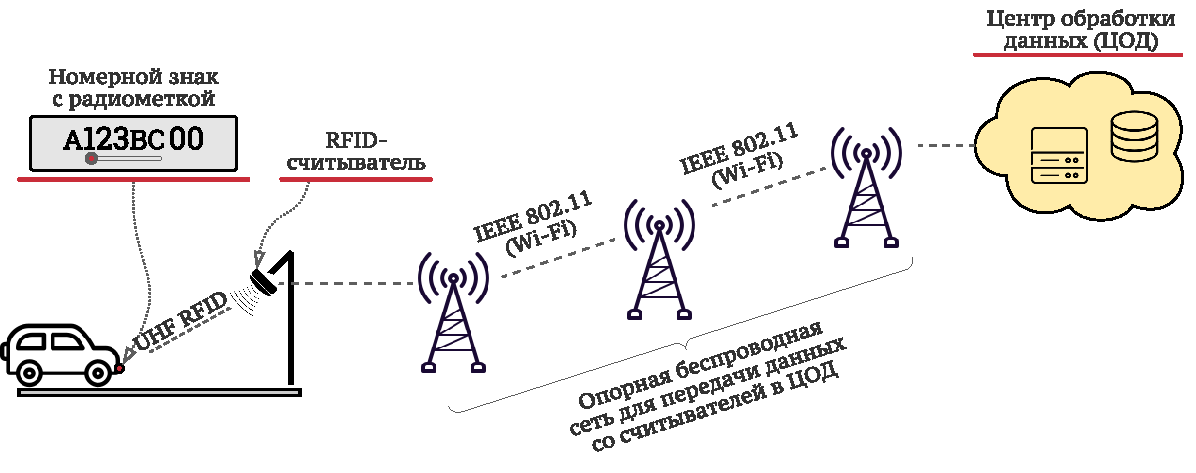
\includegraphics[width=0.9\linewidth]{chapter1/ch1_system_overview}
    \end{center}
    Система радиочастотной идентификации транспорта предназначена для
    идентификации транспорта с помощью размещенных на машинах RFID-меток
    и передачи данных по сети в центр обработки данных. Области применения:
    \begin{itemize}
        \item Повышение безопасности на дорогах "--- надежная идентификация нарушителей, поиск угнанных автомобилей
        \item Бесконтактная оплата проезда по платным дорогам
        \item Контроль доступа, оплата парковки и другие применения
    \end{itemize}
    \vfill
    \framebreak
    \begin{center}
        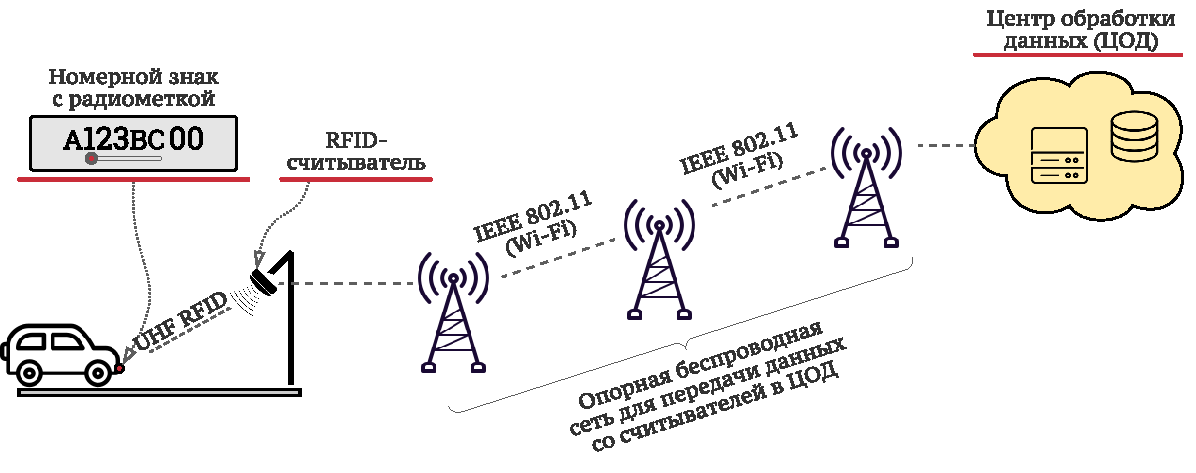
\includegraphics[width=0.9\linewidth]{chapter1/ch1_system_overview}
    \end{center}
    Система включает в себя следующие основные компоненты:
    \begin{itemize}
        \item Пассивные RFID-метки, устанавлиаемые в номера автомобилей
        \item RFID-считыватели, считывающие идентификаторы меток
        \item Сеть передачи
        \item Центр обработки данных
        \item Распределенная компьютерная система управления и сбора данных с RFID-считывателей
    \end{itemize}
\end{frame}
\note{
    Этот текст будет виден только если его отображение включено
    в~файле \textbf{Presentation/setup}.
    Для раздельного вывода презентации и заметок на~разные экраны (как
    в~impress или powerpoint) можно использовать программу
    \textit{pdf-presenter-console}.
}

\begin{frame}
    \frametitle{Постановка задач исследования}
    \begin{enumerate}
        \item Разработка и исследование комплекса аналитических и имитационных моделей для анализа и оптимизации основных характеристик систем радиочастотной идентификации транспортных средств.
        \item Разработка методики оценки производительности широкополосных беспроводных сетей, использующихся для передачи данных от RFID-считывателей в центры обработки данных, на основе методов теории массового обслуживания и марковских случайных процессов.
        \item Разработка архитектуры и реализация распределенной системы управления и сбора данных с RFID-считывателей, ее экспериментальное внедрение и проведение испытаний.
    \end{enumerate}
\end{frame}



% ============================================================================
% ЧАСТЬ 2. ИССЛЕДОВАНИЕ ПРОИЗВОДИТЕЛЬНОСТИ СИСТЕМ РАДИОЧАСТОТНОЙ ИДЕНТИФИКАЦИИ
% ============================================================================
\section{Исследование производительности систем радиочастотной идентификации}
\begin{frame}[plain, noframenumbering]
    \begin{center}
        \Huge
        Исследование производительности систем радиочастотной идентификации
    \end{center}
\end{frame}

\begin{frame}
    \frametitle{Структура системы}
    \vfill
    \begin{minipage}{0.55\linewidth}
        \begin{center}
            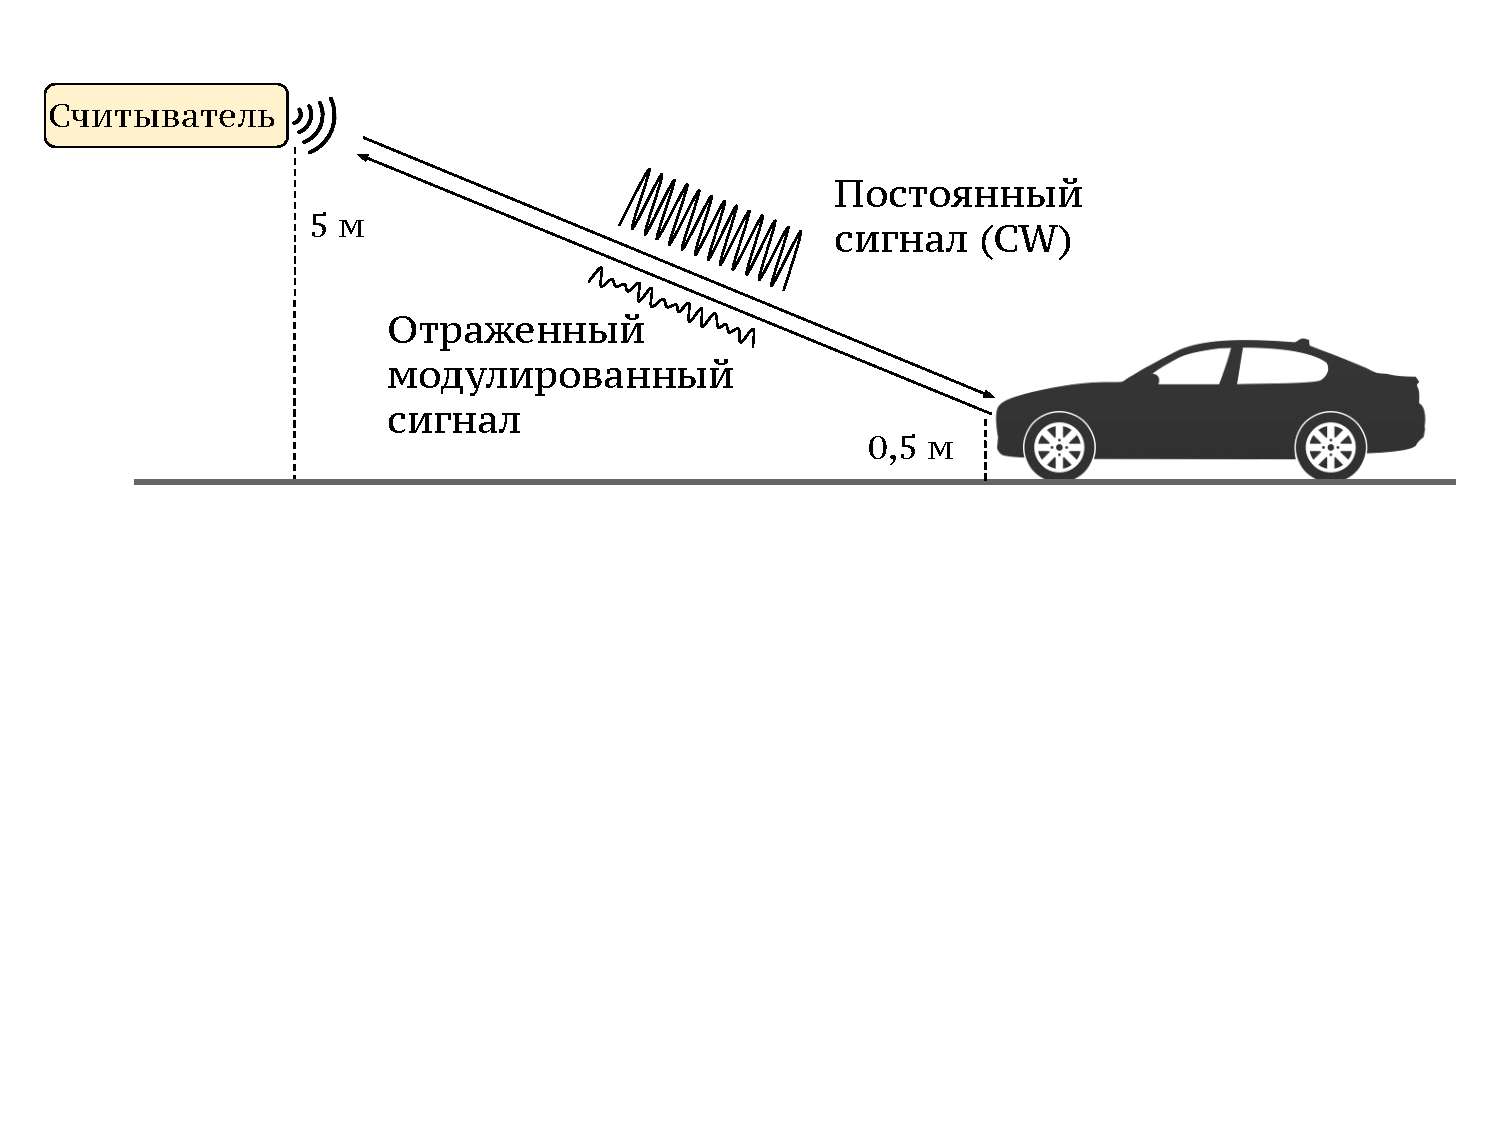
\includegraphics [scale=0.25] {chapter2/ch2_system_structure}
        \end{center}
        Между считывателем и меткой используется протокол международного стандарта EPC Class 1 Gen.2 (ISO 18006-C), диапазон 860 -- 960 МГц.
    \end{minipage}
    \hfill
    \begin{minipage}{0.4\linewidth}
        \begin{itemize}
            \item \textbf{RFID-считыватель}: создает электромагнитное поле, считывает данные с меток
            \item \textbf{Пассивные RFID-метки}: работают в области действия считывателя, модулируют отраженный сигнал
        \end{itemize}
    \end{minipage}
    \vfill
\end{frame}

\begin{frame}
    \frametitle{Протокол EPC Gen.2: физический уровень}
    \begin{center}
        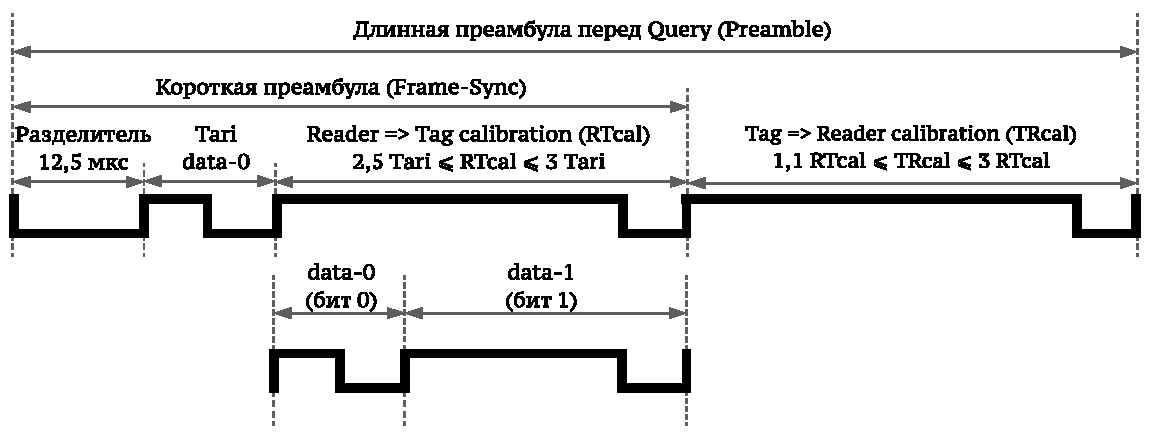
\includegraphics [width=0.9\textwidth] {chapter1/ch1_pie}
    \end{center}
    \begin{itemize}
        \item Считыватель использует кодирование PIE (Pulse Interval Encoding)
        \begin{itemize}
            \item длительность символа \textbf{data-0} равна Tari = 6,25, 12,5, 18,75 или 25 мкс
            \item длительность символа \textbf{data-1} "--- от 1,5 до 2 Tari
        \end{itemize}
        \item Метки используют код FM0 (M = 1 символ на бит) или коды миллера с M = 2, 4 или 8 символами на бит
        \item Скорость канала от метки к считывателю $\text{DR} / (\text{TRcal} * \text{M})$, DR = 8 или 64/3
        \item Выбор значений Tari, M, DR осуществляет считыватель
    \end{itemize}
\end{frame}

\begin{frame}
    \frametitle{Протокол EPC Gen.2: структура памяти метки}
    \begin{center}
        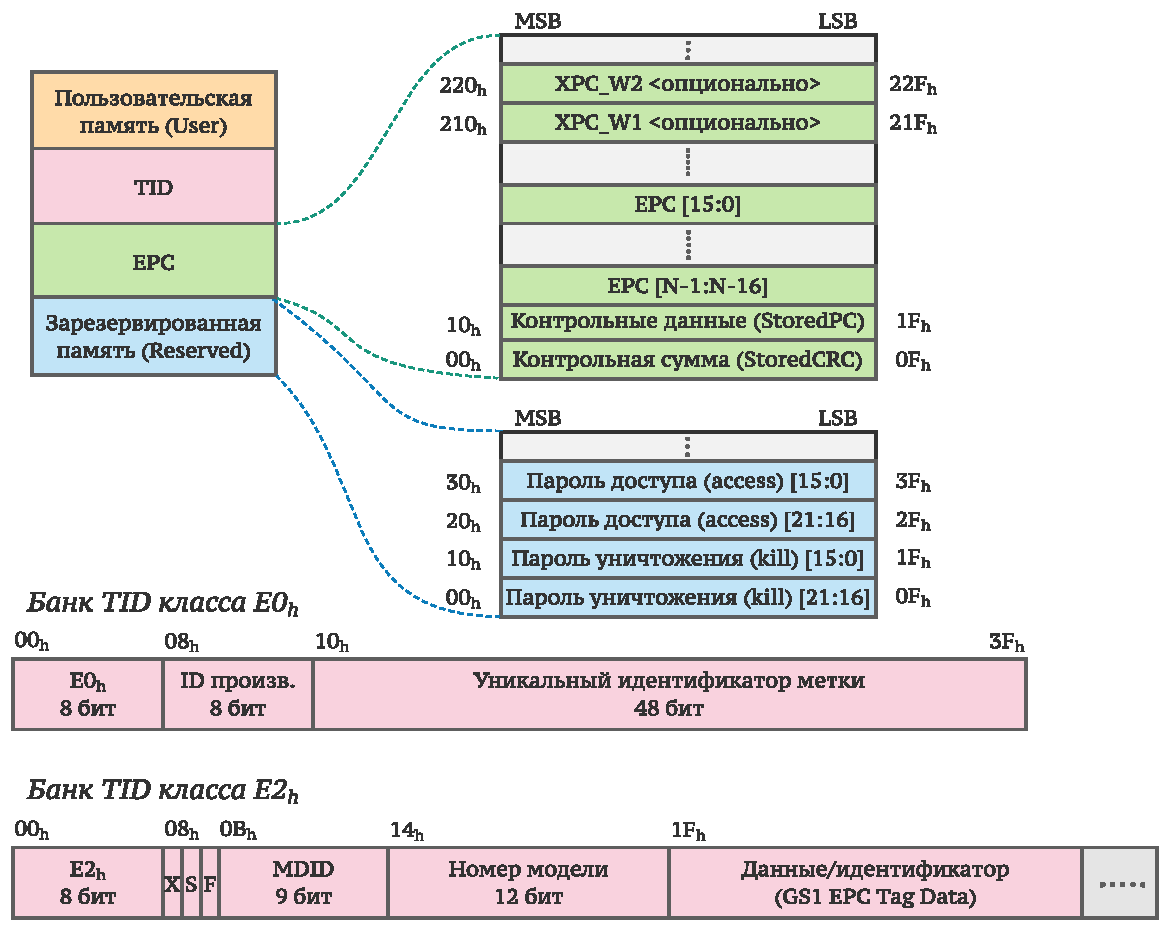
\includegraphics [width=0.75\textwidth] {chapter1/ch1_banks}
    \end{center}
    \begin{itemize}
        \item Банк EPC хранит EPCID, может быть перезаписан
        \item Банк TID записывается на фабрике, хранит уникальный номер
    \end{itemize}
\end{frame}

\begin{frame}
    \frametitle{Протокол EPC Gen.2: антиколлизионный протокол}
    \begin{center}
        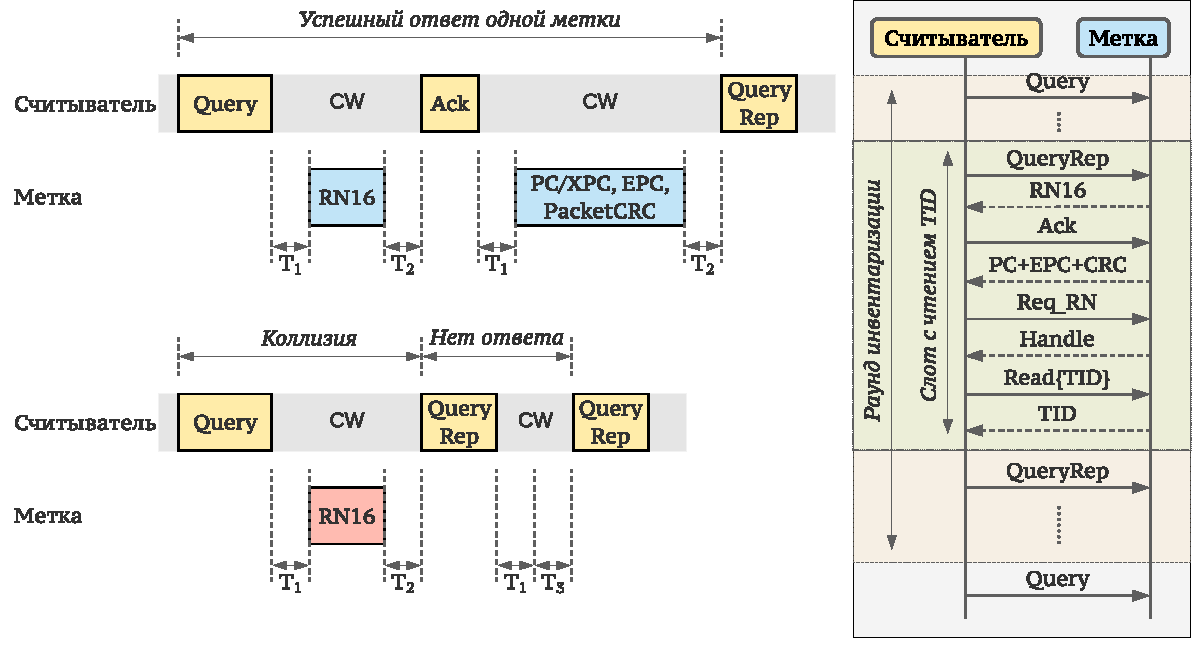
\includegraphics [width=0.75\textwidth] {chapter1/ch1_inventory}
    \end{center}
    \begin{itemize}
        \item Опрос меток орагнизован в раунды, каждый состоит из $2^Q$ слотов (слоттированная ALOHA), $0 \leqslant Q \leqslant 15$.
        \item Каждая метка выбирает случайный слот. Если один слот выбрали несколько меток, произойдет коллизия.
        \item Для чтения TID требуется передать больше сообщений, чем для чтения EPCID.
    \end{itemize}
\end{frame}

\begin{frame}
    \frametitle{Протокол EPC Gen.2: флаги сессий}
    Каждая метка хранит четрые флага сессий (значения $A$ или $B$):
    \begin{itemize}
        \item в начале раунда опроса считыватель указывает номер сессии и значение флага, которое должно быть у меток, участвующих в опросе (поле Target);
        \item если хранимое значение флага не совпадает с Target, метка не участвует в опросе.
    \end{itemize}
    \vfill
    Метка изменяет флаг:
    \begin{itemize}
        \item инвертирует после попытки передачи EPCID в ответ на Ack ($A \rightarrow B, B \rightarrow A$);
        \item сбрасывает в $A$ после при повторном включении.
    \end{itemize}
    \vfill
    Если произошла ошибка при передаче EPCID, а считыватель использует то же самое значение Target, метка не сможет повторно передать EPCID.
\end{frame}

\begin{frame}
    \frametitle{Вероятность идентификации метки}
    Вероятность идентификации RFID-метки на автомобиле можно оценить как:
    \[
        P_t \approx 1 - \left( 1 - (1 - 2^{-Q})^{N_t-1} (1 - p_e)^B \right)^{N_r},
    \]
    где
    \begin{itemize}
        \item $2^Q$ "--- число слотов в раунде опроса
        \item $N_t$ "--- среднее число меток, принимающих участие в раунде
        \item $p_e$ "--- средняя вероятность битовой ошибки (BER)
        \item $B$ "--- общее число бит в ответах метки
        \item $N_r = L / (v \tau)$ "--- среднее число раундов, в которых успевает принять метка, $L$ "--- средняя длина отрезка дороги, на котором метка получает достаточно энергии, $v$ "--- скорость движения метки, а $\tau$ "--- средняя длительность раунда инвентаризации
    \end{itemize}
    Реальное значение BER $p_e(t)$, как и величина $L$, меняются со временем, так как из-за эффекта Доплера канал оказывается зависимым от времени.
\end{frame}


\begin{frame}[allowframebreaks]
    \frametitle{Моделирование радиоканала}
    \vfill
    \begin{center}
        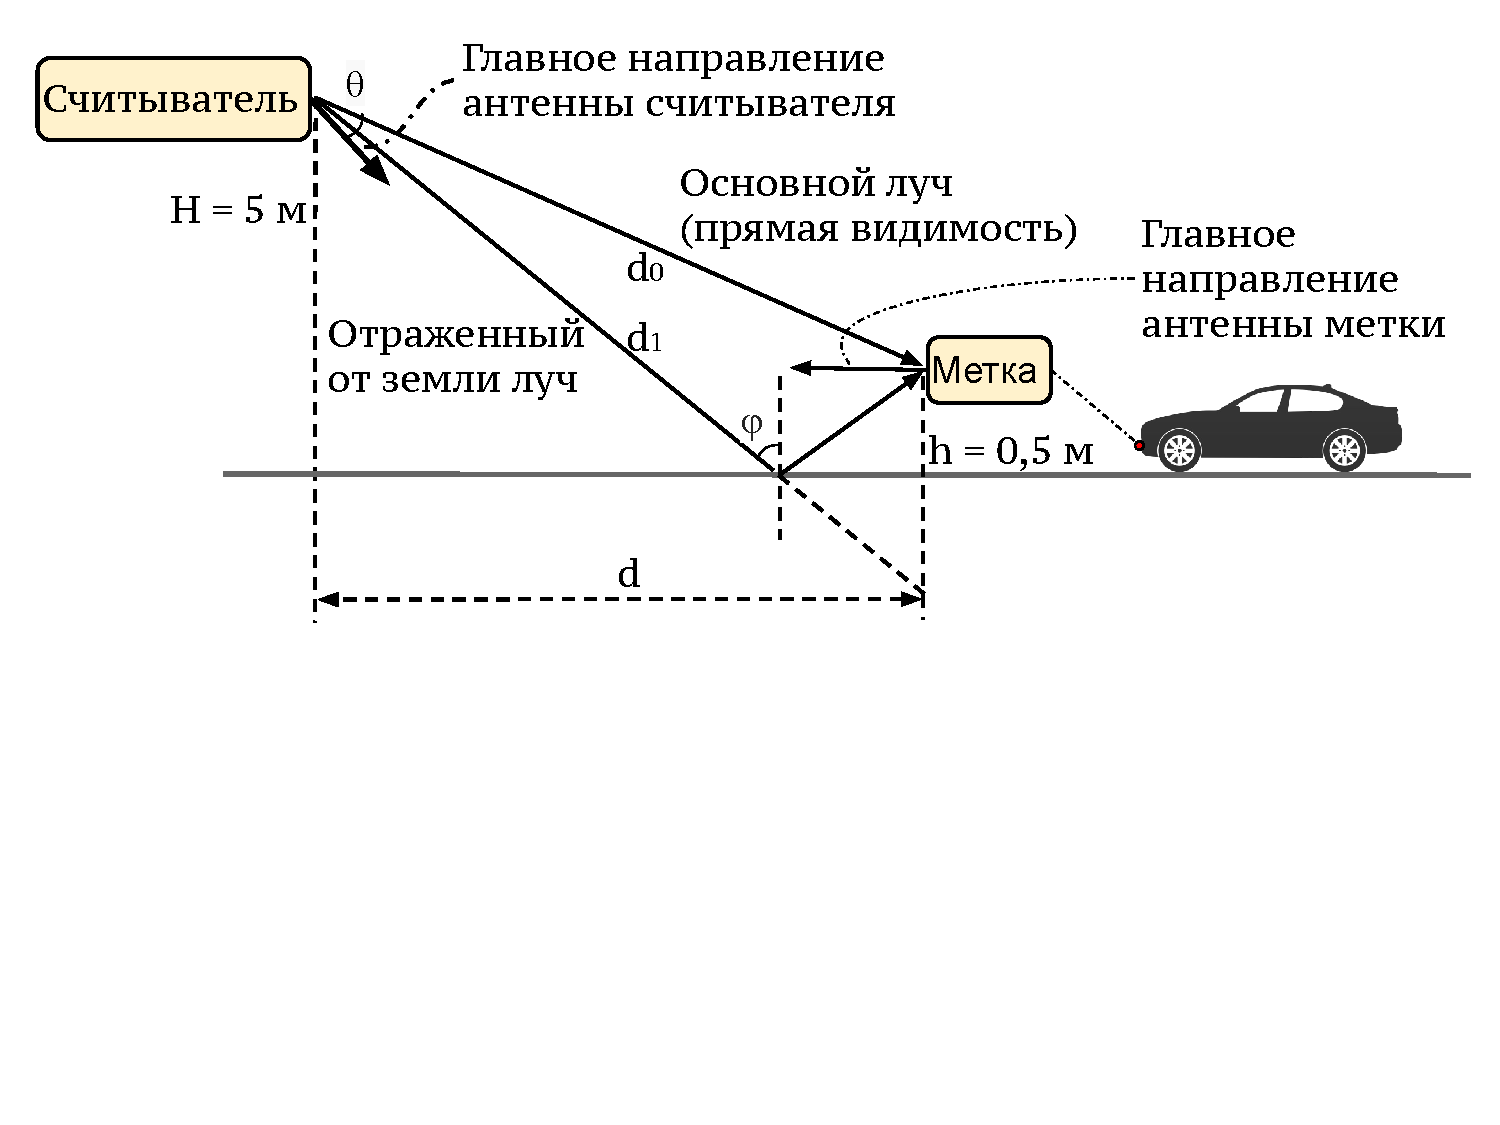
\includegraphics[width=0.8\textwidth]{chapter2/ch2_geometry}
    \end{center}
    Мощность принятого меткой сигнала считывателя:
    $$
        P_r^{(t)} = P_t^{(r)} G^{(r)} A_{pl}^{(d)} A_{pol} G^{(t)}.
    $$
    Мощность принятого считывателем отраженного сигнала:
    $$
        P_r^{(r)} = P_r^{(t)} G^{(t)} A_{bs} A_{pl}^{(r)} A_{pol} G^{(r)}.
    $$
    \vfill
    \framebreak
    \vfill
    \begin{center}
        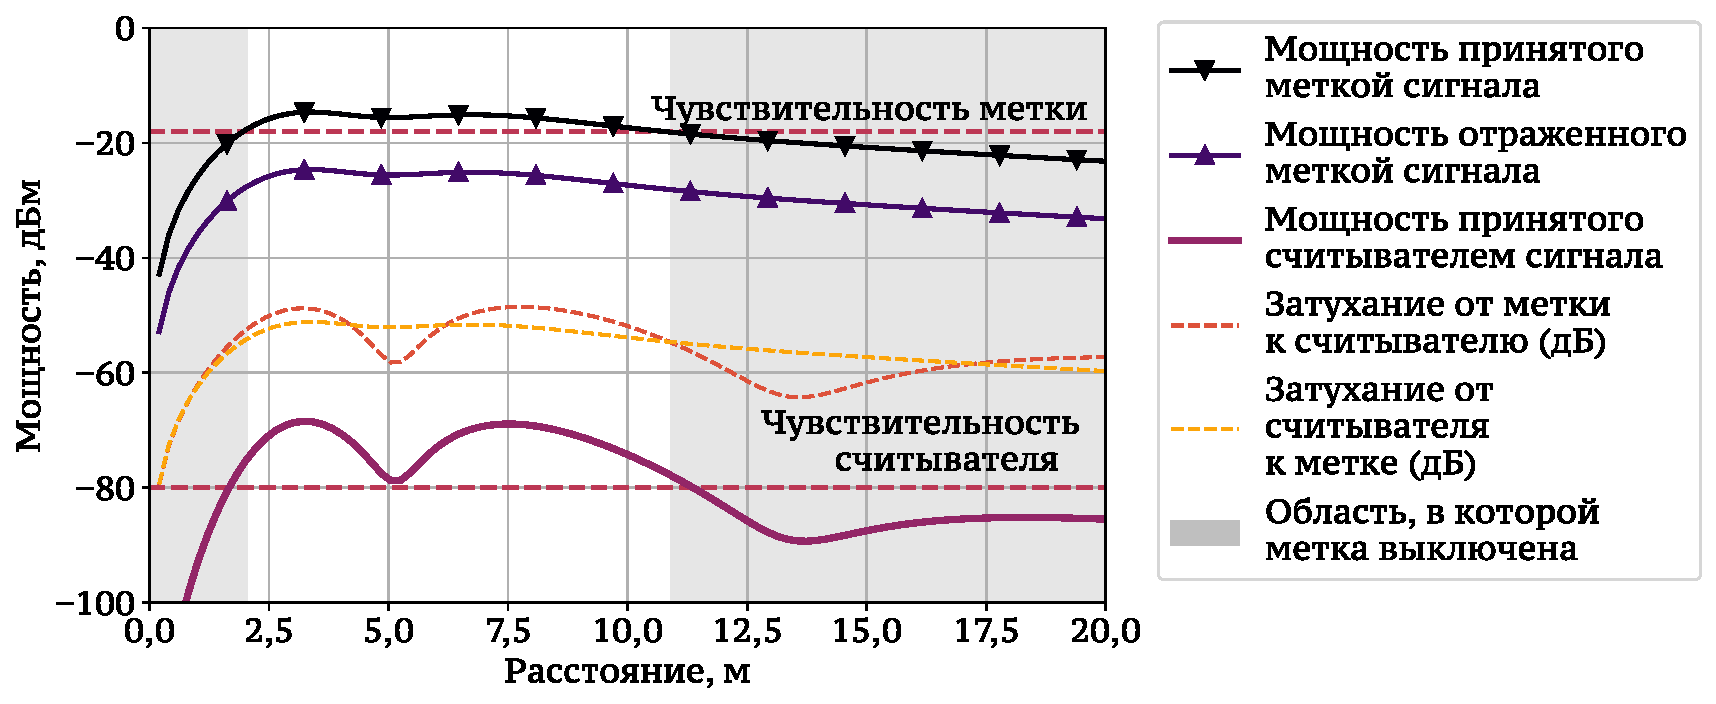
\includegraphics[width=0.99\textwidth]{chapter2/ch2_link_budget}
    \end{center}
    Затухание в канале с многолучевым распространением:
    $$
        A_{pl} = |r(t)|^2 = \left(\frac{\lambda}{4\pi}\right)^2
            \left|\sum\limits_{i=0}^{N} \frac{R_i\Gamma_i}{d_i}
            e^{-jk(d_i-\upsilon t \cos{\psi_i})}\right|^2
    $$
    \vfill
    \framebreak
    \vfill
    \begin{center}
        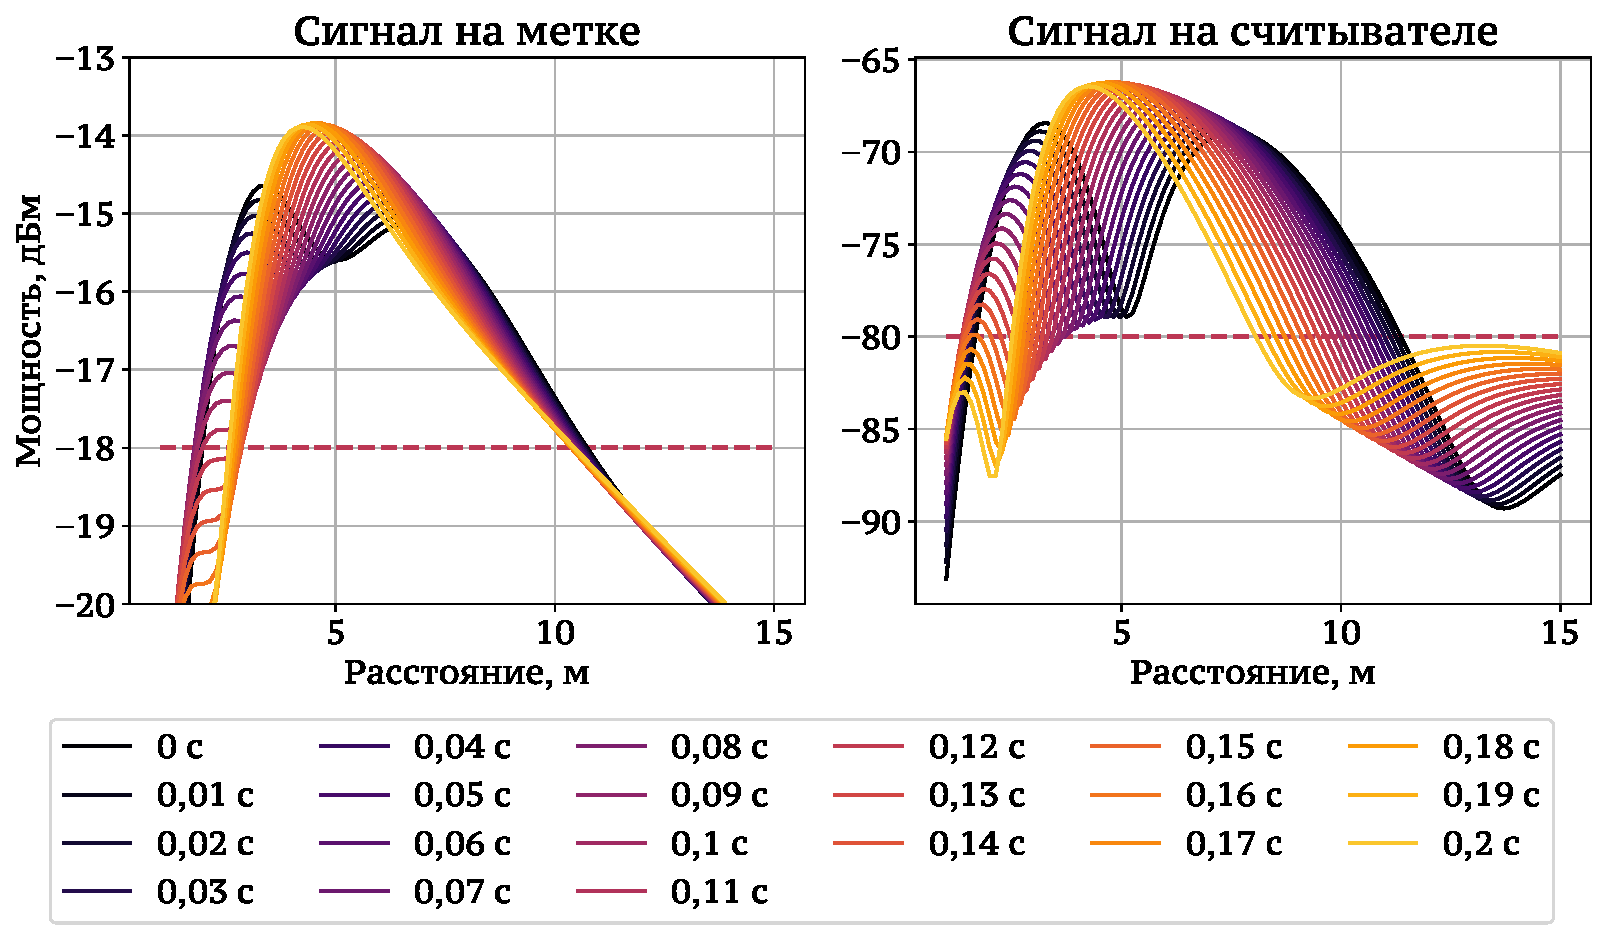
\includegraphics[width=0.99\textwidth]{chapter2/ch2_rx_power_doppler}
    \end{center}
    Существенное влияние на мощность отраженных меткой и принятых считывателем сигналов оказывает эффект Доплера.
    \vfill
  \end{frame}

% \begin{frame}[allowframebreaks]
\begin{frame}
    \frametitle{Расчет вероятности битовой ошибки (BER)}
    \begin{center}
        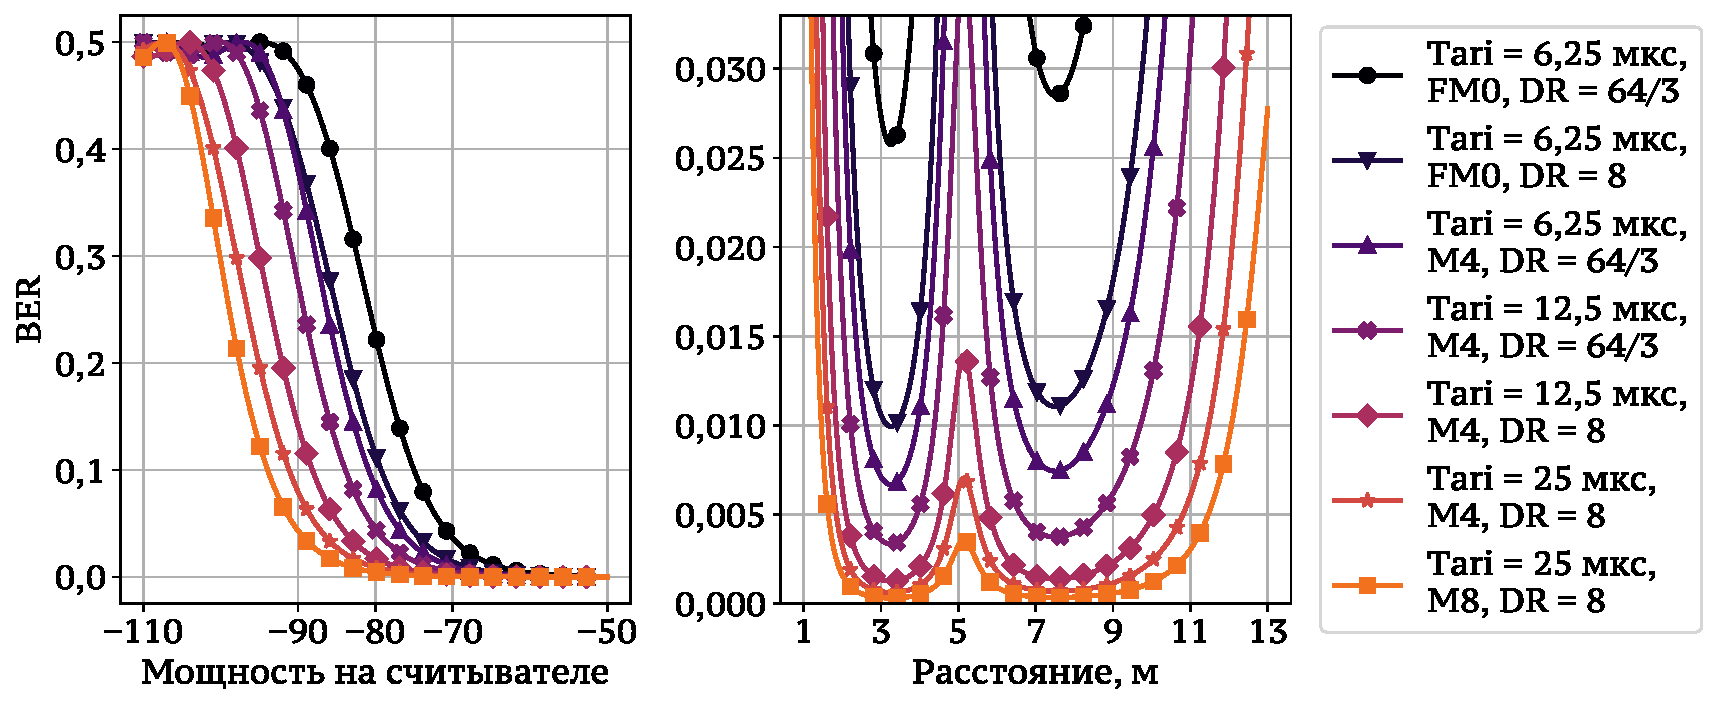
\includegraphics[width=0.9\textwidth]{chapter2/ch2_ber}
    \end{center}
    $$
	    P_{er} = \frac{1}{2} - \frac{1}{\sqrt{1+\frac{2}{\acute{\gamma}}}} +
		    	 \frac{2}{\pi}\frac{\arctan{\sqrt{1+\frac{2}{\acute{\gamma}}}}}{1+\frac{2}{\acute{\gamma}}},
    $$
    где $\acute{\gamma} = mE_s/N_0\cos^2{\phi_s}$; $m$ "--- число символов на бит (порядок) в коде Миллера, $E_s$ "--- энергия одного символа, $N_0/2$ "--- спектральная плотность белого шума и $\phi_s$ "--- разность между реальной и принятой фазами сигнала
    \vfill
    % \framebreak
    % \vfill
    % \begin{center}
    %     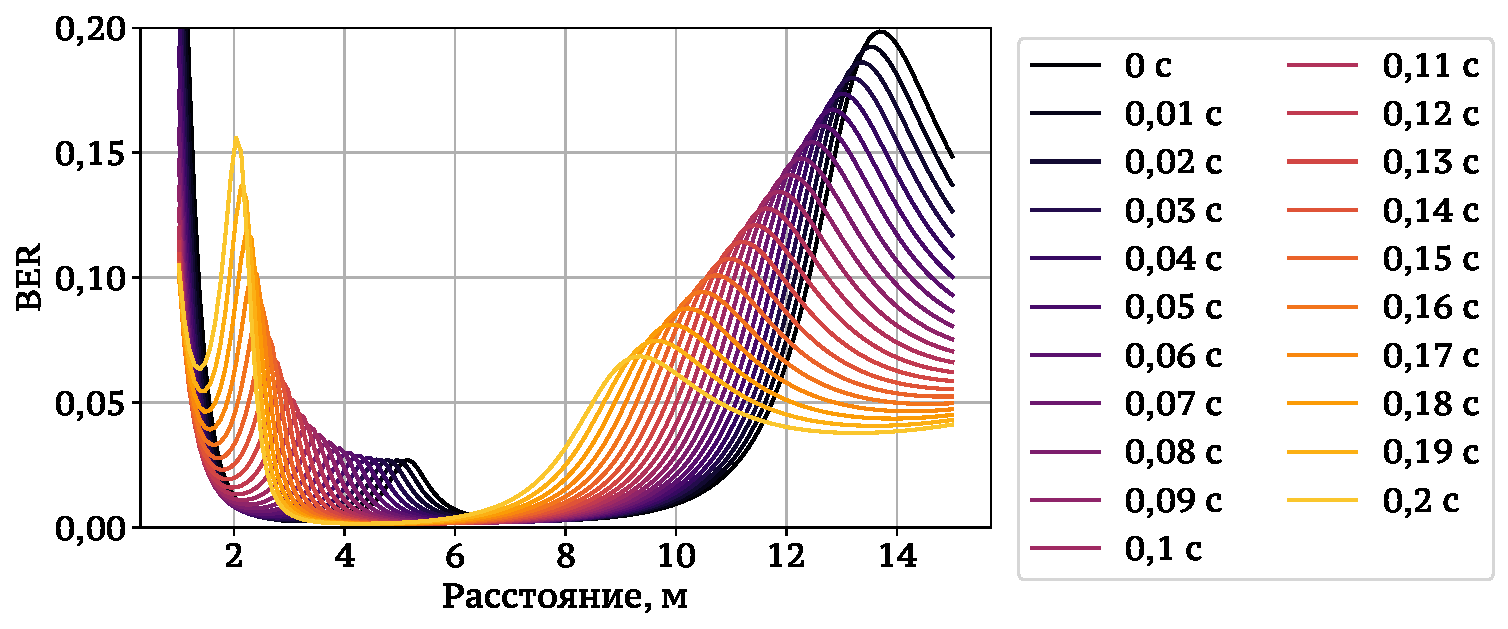
\includegraphics[width=0.99\textwidth]{chapter2/ch2_ber_doppler.pdf}
    % \end{center}
    % Существенное влияние на BER оказывает эффект Доплера.
\end{frame}


\begin{frame}
    \frametitle{Оценка максимального числа раундов опроса}
    \begin{center}
        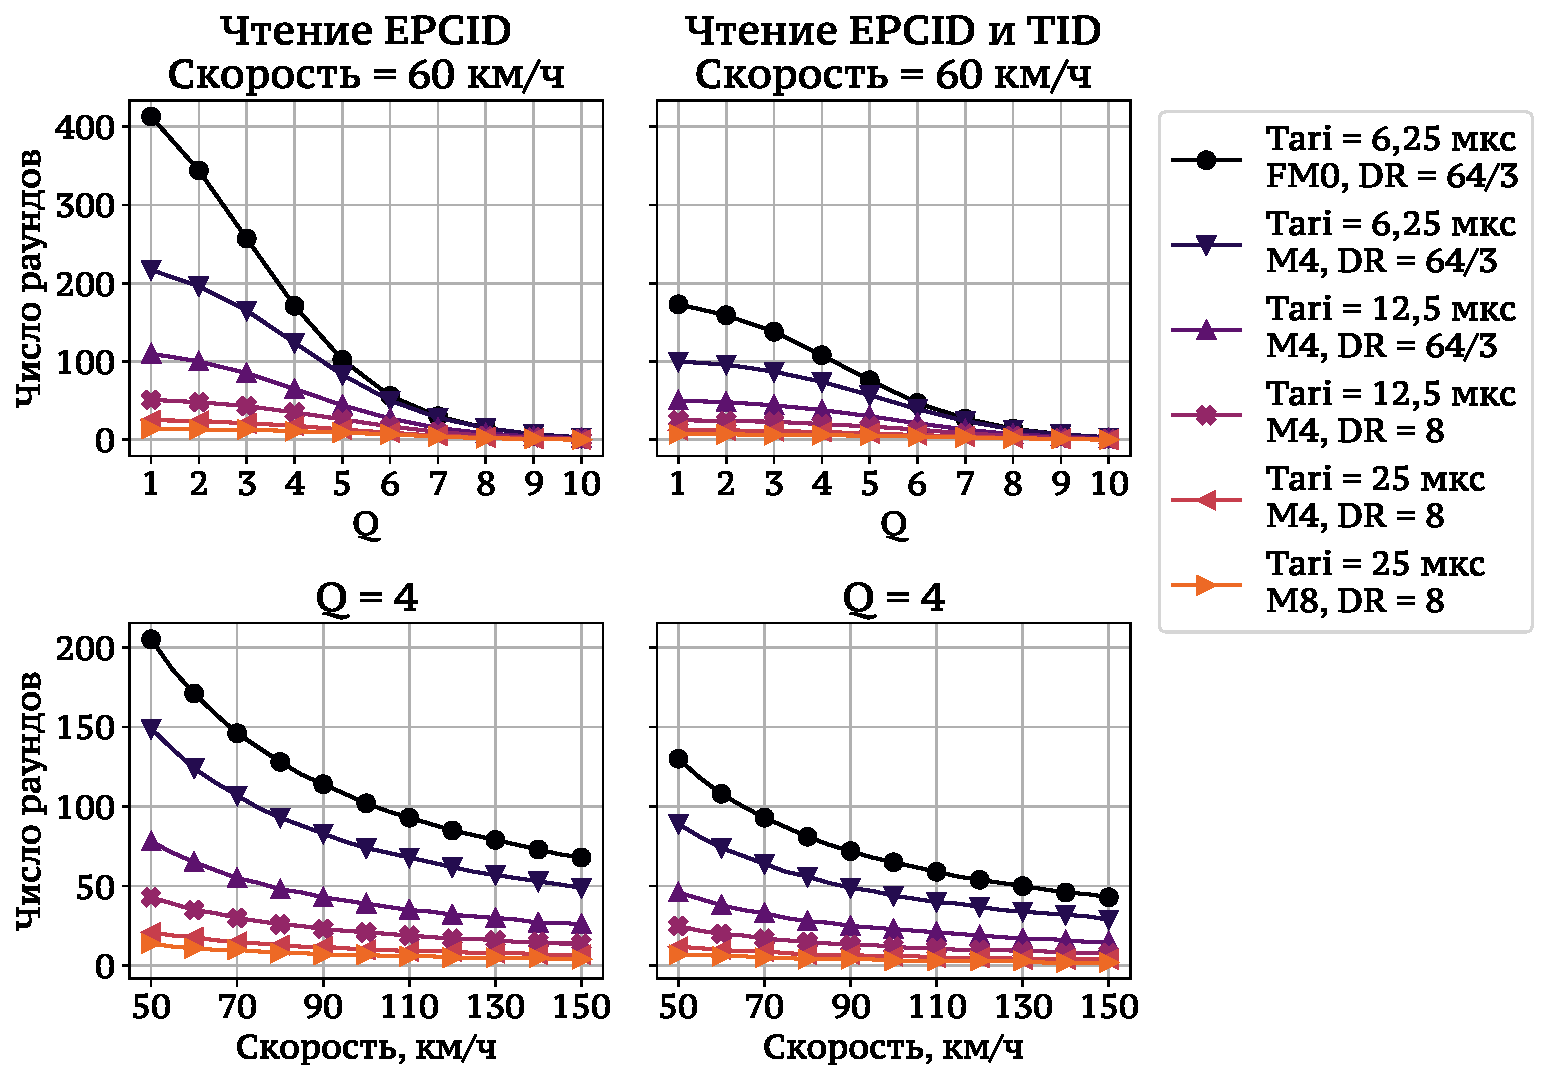
\includegraphics[width=0.8\textwidth]{chapter2/ch2_max_num_rounds.pdf}
    \end{center}
    Длительности команд и ответов существенно зависят от выбранных параметров протокола Tari, M, DR. Из-за этого число раундов опроса, в которых метка может принять участие, может меняться в очень широком диапазоне.
\end{frame}

\begin{frame}
    \frametitle{Разработанная имитационная модель}
    Для получения численных результатов при различных настройках считывателей и параметрах окружения была разработана имитационная дискретно-событийная модель. Особенности:

    \begin{itemize}
        \item точный расчет длительности команд, учитывающий кодирование PIE;
        \item учет изменения BER в течение передачи ответов;
        \item моделирование периодических отключений считывателя;
        \item поддержка произвольного числа полос движения и направлений антенн;
        \item учет стратегии выбора флагов сессий для опроса меток;
        \item сбор и анализ различных показателей модели: вероятности идентификации меток, число раундов опроса, в которых участвует метка, число меток в раундах опроса;
        \item высокая гибкость: поддерживает более 50 параметров.
    \end{itemize}

    Модель реализована на языке Python 3, открытый исходный код: \url{https://github.com/larioandr/thesis-rfidsim}
\end{frame}

\begin{frame}
    \frametitle{Результаты: число раундов}
    \begin{center}
        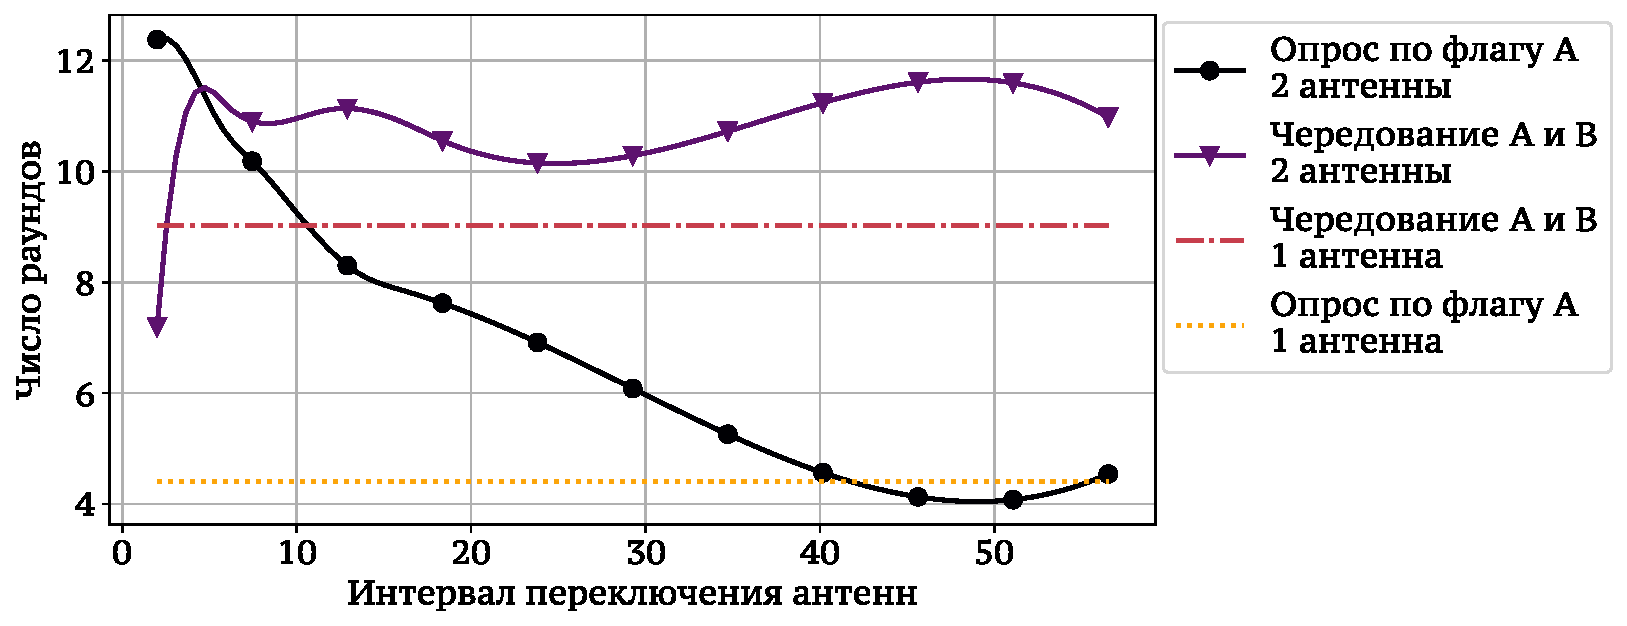
\includegraphics[width=0.9\textwidth]{chapter2/ch2_sim_num_rounds_one_lane}
    \end{center}
    \begin{itemize}
    \item При передаче EPCID метками часто происходят ошибки, из-за инверсии флага сессии метки не могут повторно принять участие в опросе до выключения.
    \item При переключении считывателем антенн часть меток выключается, что ведет к сбросу флага сессии.
    \item Чередование опрашиваемых флагов сессии позволяет эффективно повысить число раундов, в которых метка принимает участие.
    \end{itemize}
\end{frame}

\begin{frame}
    \frametitle{Влияние выбора Tari на вероятность идентификации}
    \begin{center}
        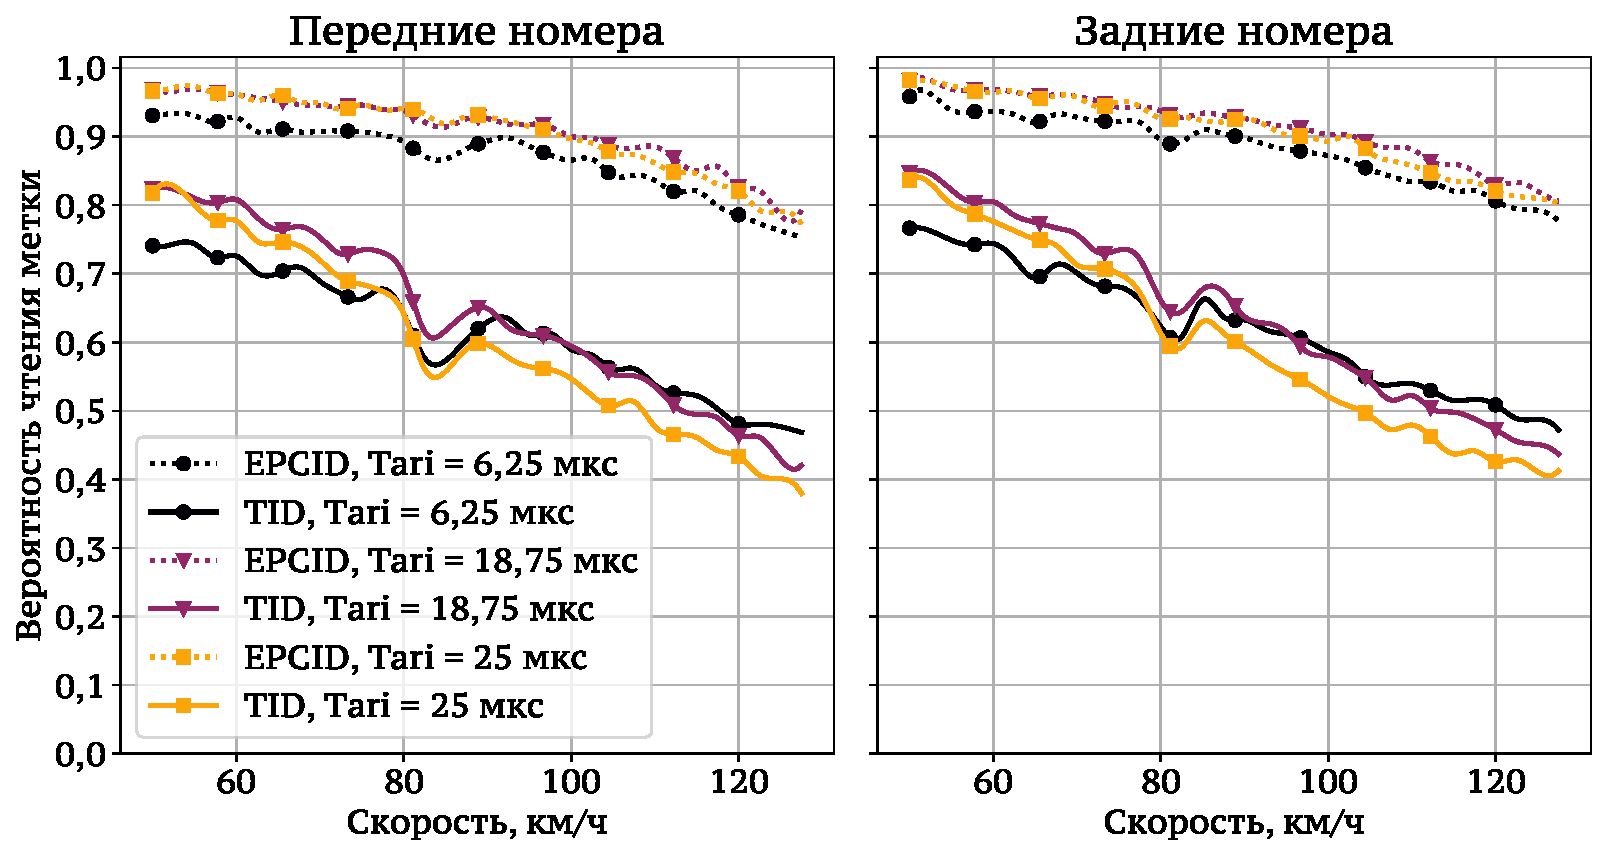
\includegraphics[width=0.8\textwidth]{chapter2/ch2_tag_identification_m4}
    \end{center}
    На графике "--- вероятности идентификации меток при M = 4.
    \begin{itemize}
    \item При низкой скорости эффективнее использовать длинные символы в командах считывателя (Tari = 18,75~мкс)
    \item При высокой скорости более высокая вероятность идентификации при коротких символах (Tari = 6,25~мкс).
    \end{itemize}
\end{frame}

\begin{frame}
    \frametitle{Влияние длины ответов на вероятность идентификации}
    \begin{center}
        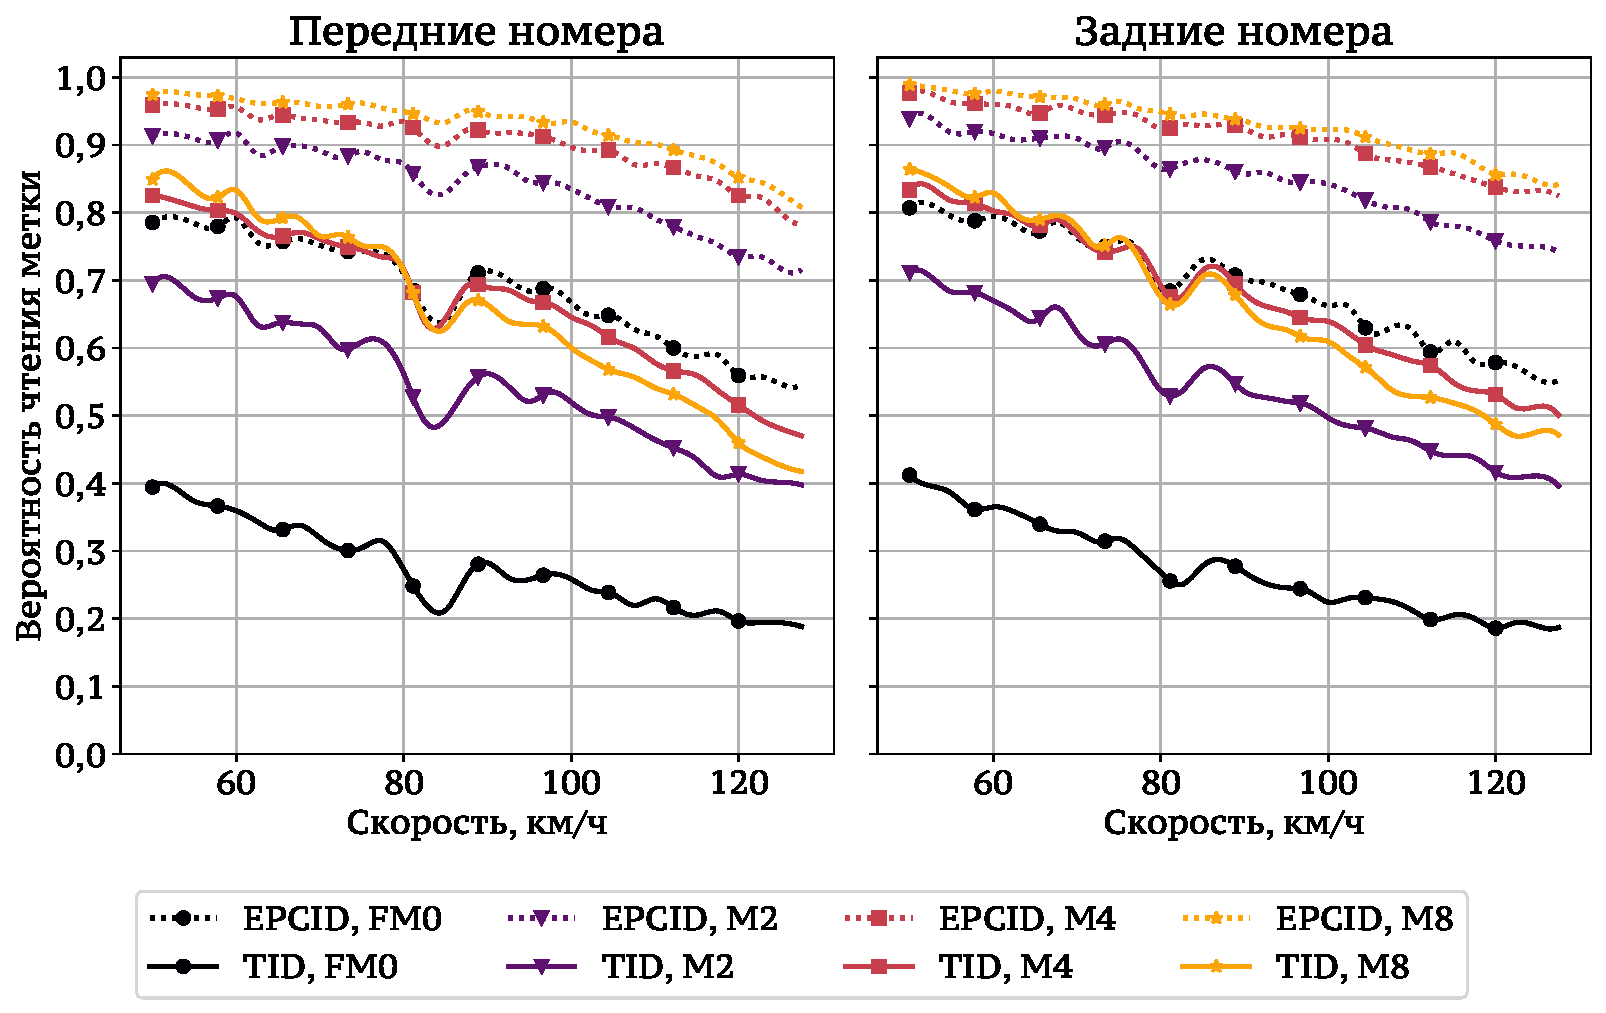
\includegraphics[width=0.8\textwidth]{chapter2/ch2_tag_identification_tari125}
    \end{center}
    \begin{itemize}
        \item При низкой скорости эффективнее использовать код c M = 8 симолов на бит, при высокой "--- M = 2.
        \item При использовании самого быстрого и ненадежного кода FM0 (M = 1) вероятность идентификации слишком низкая.
    \end{itemize}
\end{frame}

\begin{frame}
    \frametitle{Вероятность идентификации автомобиля}
    \begin{center}
        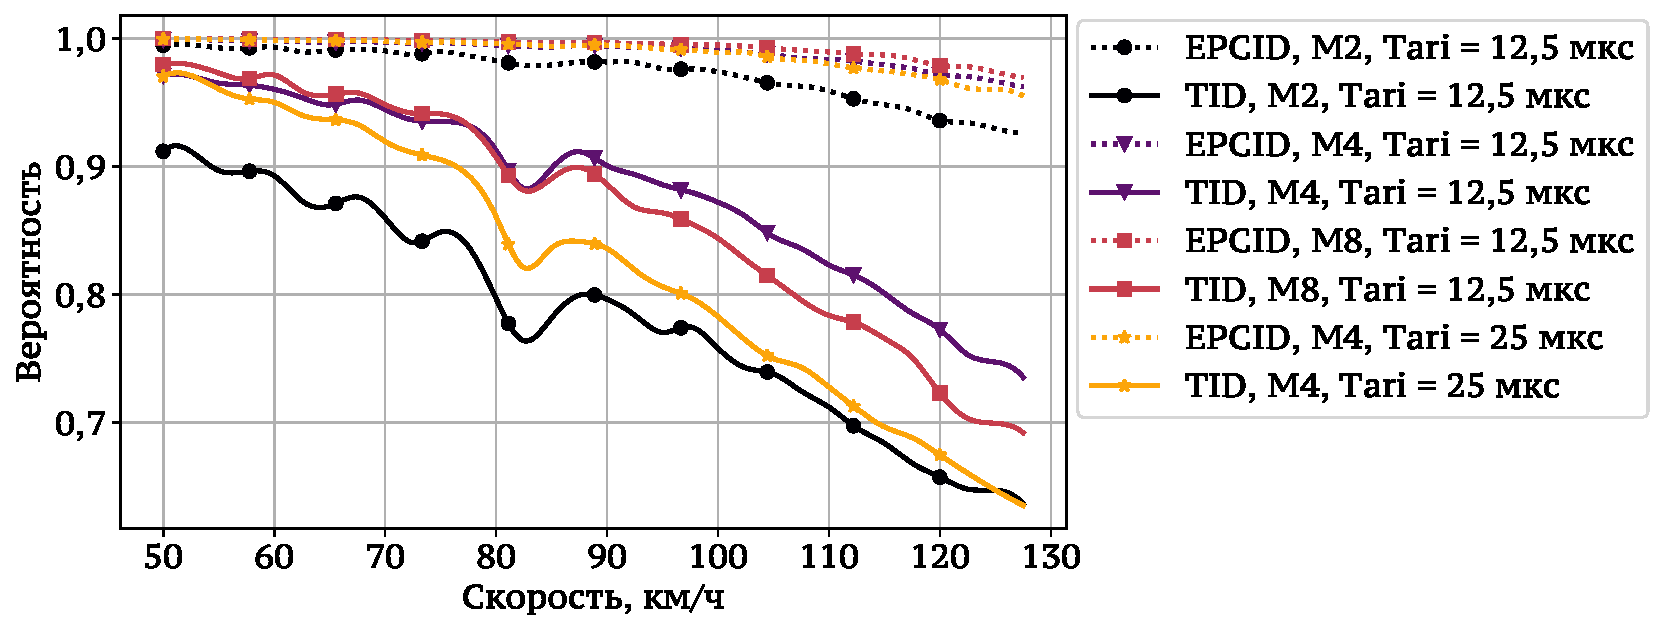
\includegraphics[width=0.85\textwidth]{chapter2/ch2_vehicle_identification_rate}
    \end{center}
    \begin{itemize}
        \item Автомобиль идентифицируется по любой из меток (в переднем или заднем номере).
        \item Самая высокая вероятность идентификации достигается при использовании M = 4 символа на бит в ответах метки и Tari = 12,5~мкс:
        \begin{itemize}
            \item если Tari = 25~мкс или M = 8, раунды опроса становятся слишком длинными;
            \item если M = 1 или M = 2, то вероятность битовой ошибки слишком высока.
        \end{itemize}
    \end{itemize}

\end{frame}

\begin{frame}
    \frametitle{Выводы}
    \begin{itemize}
        \item Выделены факторы, влияющие на вероятность успешной идентификации меток.
        \item Предложена имитационная модель, учитывающая различные сценарии идентификации автомобилей, учитывающая настройки протокола, параметры окружения и особенности распространения радиосигналов вблизи автодороги.
        \item С помощью имитационной модели получены зависимости вероятности идентификации как отдельных номеров, так и автомобилей, от скорости движения и выбранных настроек протокола EPC Class 1 Gen.2.
        % \item Результаты были опубликованы в журнале IEEE Journal on RFID, а также представлены и опубликованы в трудах конференций IEEE RFID 2017 (США) и DCCN (Россия).
    \end{itemize}
\end{frame}



% ============================================================================
% ЧАСТЬ 3. АНАЛИТИЧЕСКАЯ МОДЕЛЬ СИСТЕМЫ РАДИОЧАСТОТНОЙ ИДЕНТИФИКАЦИИ
% ============================================================================
\section{Аналитическая модель системы радиочастотной идентификации}
\begin{frame}[plain, noframenumbering]
    \begin{center}
        \Huge
        Аналитическая модель системы радиочастотной идентификации
    \end{center}
\end{frame}

\begin{frame}
    \frametitle{Сбросы питания считывателя и флаги в RFID}
    Каждая метка хранит четрые флага сессий (значения $A$ или $B$):
    \small
    \begin{itemize}
        \item в начале раунда опроса считыватель указывает номер сессии и значение флага, которое должно быть у меток, участвующих в опросе (поле Target);
        \item если хранимое значение флага не совпадает с Target, метка не участвует в опросе.
    \end{itemize}
    \vfill
    Метка изменяет флаг:
    \small
    \begin{itemize}
        \item инвертирует после попытки передачи EPCID в ответ на Ack ($A \rightarrow B, B \rightarrow A$);
        \item сбрасывает в $A$ после при повторном включении.
    \end{itemize}
    \vfill
    Если произошла ошибка при передаче EPCID, а считыватель использует то же самое значение Target, метка не сможет повторно передать EPCID.
    \begin{block}{}
        Выбор последовательности значений флага (Target) и приодические сбросы питания RFID-считывателем оказывают существенное влияние на число раундов опроса, в которых участвует метка.
    \end{block}
\end{frame}

\begin{frame}
    \frametitle{Постановка задачи}

    \begin{block}{}
    \textit{Спецификацией раунда} будем называть пару значений опрашиваемого флага и признака сброса питания $(X, e)$, которую будем сокращенно обозначать символом $\alpha = X^{e}$.
    \end{block}

    \begin{block}{}
    \textit{Сценарием работы считывателя} $\bm{\alpha} = \alpha_1 \alpha_2 \dots \alpha_R$ будем называть последовательность спецификаций раундов конечной длины $R$.
    \end{block}

    \begin{alertblock}{Задача}
        Пусть известны законы движения меток $x_i(t) \equiv x(t - t_i)$, вероятность битовой ошибки в передаче ответов $\beta$ и сценарий работы считывателя $\bm{\alpha} = \alpha_1 \alpha_2 \dots \alpha_R$, а также размеры и длительности команд считывателя и ответов меток. Пусть также для идентификации меток требуется только EPCID (или комбинация EPCID и TID). Требуется найти вероятность, с которой каждая метка будет успешно идентифицирована.
    \end{alertblock}
\end{frame}

\begin{frame}
    \frametitle{Случайные процессы}
    Для моделирования поведения системы предлагается использовать два неоднородных марковских случайных процесса:
    \small
    \begin{enumerate}
        \item $\{ \eta_r \}$ "--- число меток, участвующих в $r$-м раунде опроса (\textit{фоновый процесс});
        \item $\{( \eta_r, \phi_r^{[r_0]} )\}$ "--- случайный процесс, описывающий одновременное изменение числа активных меток $\eta_r$ и изменение состояния выделенной (наблюдаемой) метки $\phi_r^{[r_0]}$, поступившей в $r_0$-м раунде опроса (\textit{основной процесс}). Вторая компонента принимает значения:
        \footnotesize
        \begin{itemize}
            \item $\phi_r^{[r_0]} = 0$, если выделенная метка неактивна;
            \item $\phi_r^{[r_0]} = 1$, если выделенная метка активна;
            \item $\phi_r^{[r_0]} = 2$, если выделенная метка хотя бы раз успешно передала идентификатор (поглощающее состояние).
        \end{itemize}
    \end{enumerate}
    \begin{block}{}
        \small
        Вероятность идентификации произвольной метки $P_X$ вычисляется как вероятность перехода в поглощающее состояние процесса $\phi_r^{[r_0]}$ за число раундов $Q_{r_0}$, в течение которых метка, поступившая в раунде $r_0$, находится в области действия считывателя, усредненное по номерам раундов $r_0 = \overline{1, R}$.
    \end{block}
\end{frame}

\begin{frame}
    \frametitle{Алгоритм расчета вероятности идентификации}
    \footnotesize
    \begin{enumerate}
        \item Вычисляются начальные оценки длительностей раундов $\bm{\tau} = (\tau_1, \tau_2, \dots, \tau_R)$ по заданному сценарию работы считывателя $\bm{\alpha}$.
        \item По известным оценкам длительностей раундов $\bm{\tau}$ и функции числа меток в системе от времени $N = f(t)$ строится последовательность элементарных операций $U^{\nabla}_N$, $U^{\times}_N$, $U^{\downarrow}_N$, $U^{+}_N$, $U^{-}_N$. Каждому раунду соответствует композиция нескольких операций.
        \item С помощью последовательности операций вычисляются переходные вероятности фонового случайного процесса $\{\eta_r\}$, описывающего изменение числа активных (участвующих в опросе) меток в области чтения. С помощью этого процесса вычисляется стационарное распределение числа меток, участвующих в каждом раунде, $\bm{\pi}^{(r)}, r = \overline{1,R}$.
        \item По найденным распределениям числа меток $\bm{\pi}^{(r)}$ вычисляются новые оценки длительностей раундов $\bm{\tau}' = (\tau'_1, \tau'_2, \dots, \tau'_R)$. Если отклонение $\sigma = (\sum_{r=1}^R (\tau'_r - \tau_r)^2 / R)^{1/2} < \epsilon$, то переход на шаг 5, в противном случае "--- на шаг 2.
        \item Находятся переходные вероятности основного случайного процесса $\{ \eta_r, \phi_r^{[r_0]} \}$, описывающего состояние наблюдаемой метки для каждого $r_0$.
        \item Рассчитывается вероятность поглощения основного процесса и вычисляется вероятность идентификации метки $P_X$.
    \end{enumerate}
\end{frame}

\begin{frame}
    \frametitle{Расчет длительностей раундов опроса}
    Длительность раунда опроса можно оценить как:
    $$
    \tau_r(n) = N_s \sum\limits_{i=0}^{2}p_i(n)t_i +
		(T_\text{Query} - T_\text{QRep}) +
		e_r T_\downarrow
    $$
    \footnotesize
    \begin{itemize}
        \item $n$ "--- число меток, участвующих в раунде (\textit{активных меток})
        \item $T_{\text{msg}}$ "--- длительность команды или ответа
        \item $N_s$ "--- число слотов в раунде опроса
        \item $e_r$ "--- признак сброса питания после раунда опроса
        \item $T_\downarrow$ "--- длительность сброса питания после раунда
        \item $p_i(n)$ "--- вероятность того, что слот пуст ($i = 0$), содержит ответ одной метки ($i = 1$) или коллизию ($i = 2$)
        \item $t_i$ "--- длительность слота $i$-го типа
    \end{itemize}
    \begin{block}{Средняя длительность раунда}
        Если известно распределение числа активных меток $\bm{\pi}$, то:
        $$
        \tau_r = \sum\limits_{n=0}^{\overline{N}} \pi_n \tau_r(n).
        $$
    \end{block}
\end{frame}

\begin{frame}
    \frametitle{Размеченные сценарии}
    \small
    Если известны оценки длительностей раундов $\bm{\tau} = (\tau_1, \tau_2, \dots, \tau_R)$ и закон изменения числа меток в области действия считывателя $N = f(t)$, то для заданного сценария $\bm{\alpha}$ можно построить \textit{размеченный сценарий} $\widetilde{\bm{\alpha}}$.

    \small
    \begin{block}{}
        Будем называть \textit{размеченным сценарием} последовательность символов $\widetilde{\bm{\alpha}} = \widetilde{\alpha}_1 \widetilde{\alpha}_2 \dots \widetilde{\alpha}_R$, каждый из которых имеет вид пятерки $\alpha_r = (X_r, e_r ; N_r, \Delta^-_r, \Delta^+_r)$. Символы $\alpha_r$ будем называть \textit{размеченными спецификациями раундов} и использовать обозначение $[\prescript{N_r}{\Delta_r^-} X_{\Delta_r^+}^{e_r}]$, причем для сокращения записи можно опускать $\Delta_r^-$, $\Delta_r^+$ и $e_r$, если они равны нулю.
    \end{block}

    \footnotesize
    \begin{itemize}
        \item $X_r$: значение флага сессии, по которому происходит опрос, $X=A,B$;
        \item $e_r$: признак отключения считывателя после опроса;
        \item $N_r = f(\tau_1 + \dots \tau_{r-1})$: число меток, находящихся в области чтения;
        \item $\Delta^-_r$: число меток, покинувших область чтения за время раунда;
        \item $\Delta^+_r$: число меток, поступивших в область чтения за время раунда.
    \end{itemize}
\end{frame}

\begin{frame}
    \frametitle{Элементарные операции}
    \begin{center}
        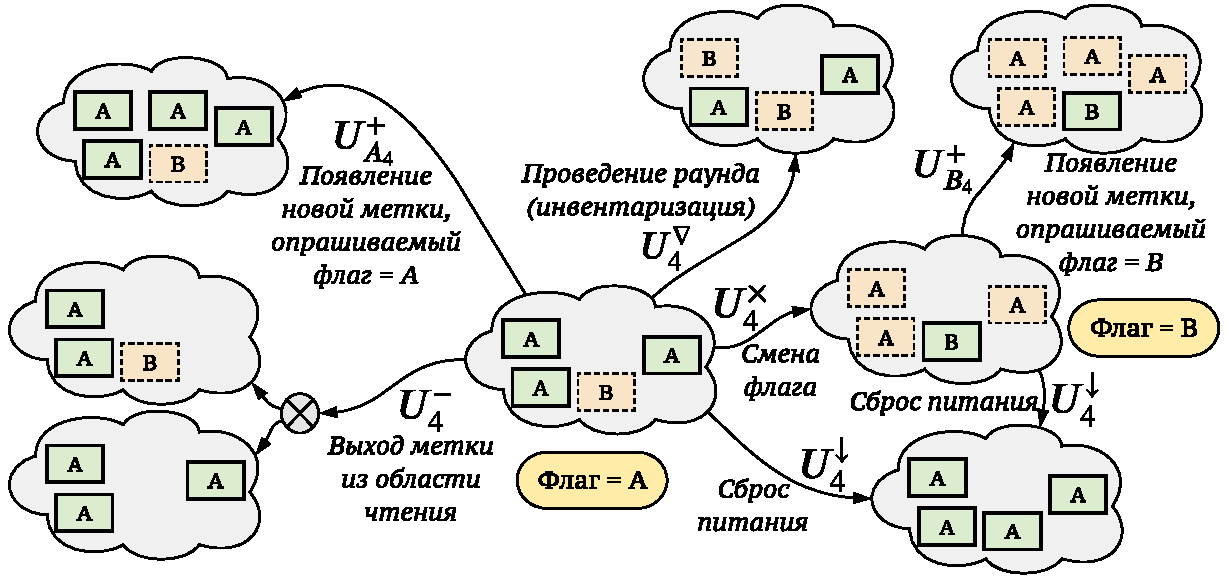
\includegraphics[width=0.8\textwidth]{chapter3/ch3_operations.pdf}
    \end{center}
    \small
    Изменение состояния системы описывается с помощью последовательности элементарных операций, однозначно определяемой по найденному размеченному сценарию. Пять типов операций:
    \footnotesize
    \begin{itemize}
        \item $U^\nabla_N$: проведение раунда опроса с $N$ активными метками;
        \item $U^\times_N$: смена флага опроса считывателем;
        \item $U^\downarrow_N$: выключение питания считывателем;
        \item $U^+_{X_N}$: появление в области действия считывателя новой метки, $X = A,B$;
        \item $U^+_N$: выход метки из области действия счиытвателя.
    \end{itemize}
\end{frame}

\begin{frame}
    \frametitle{Композиция элементарных операций}
    \begin{center}
        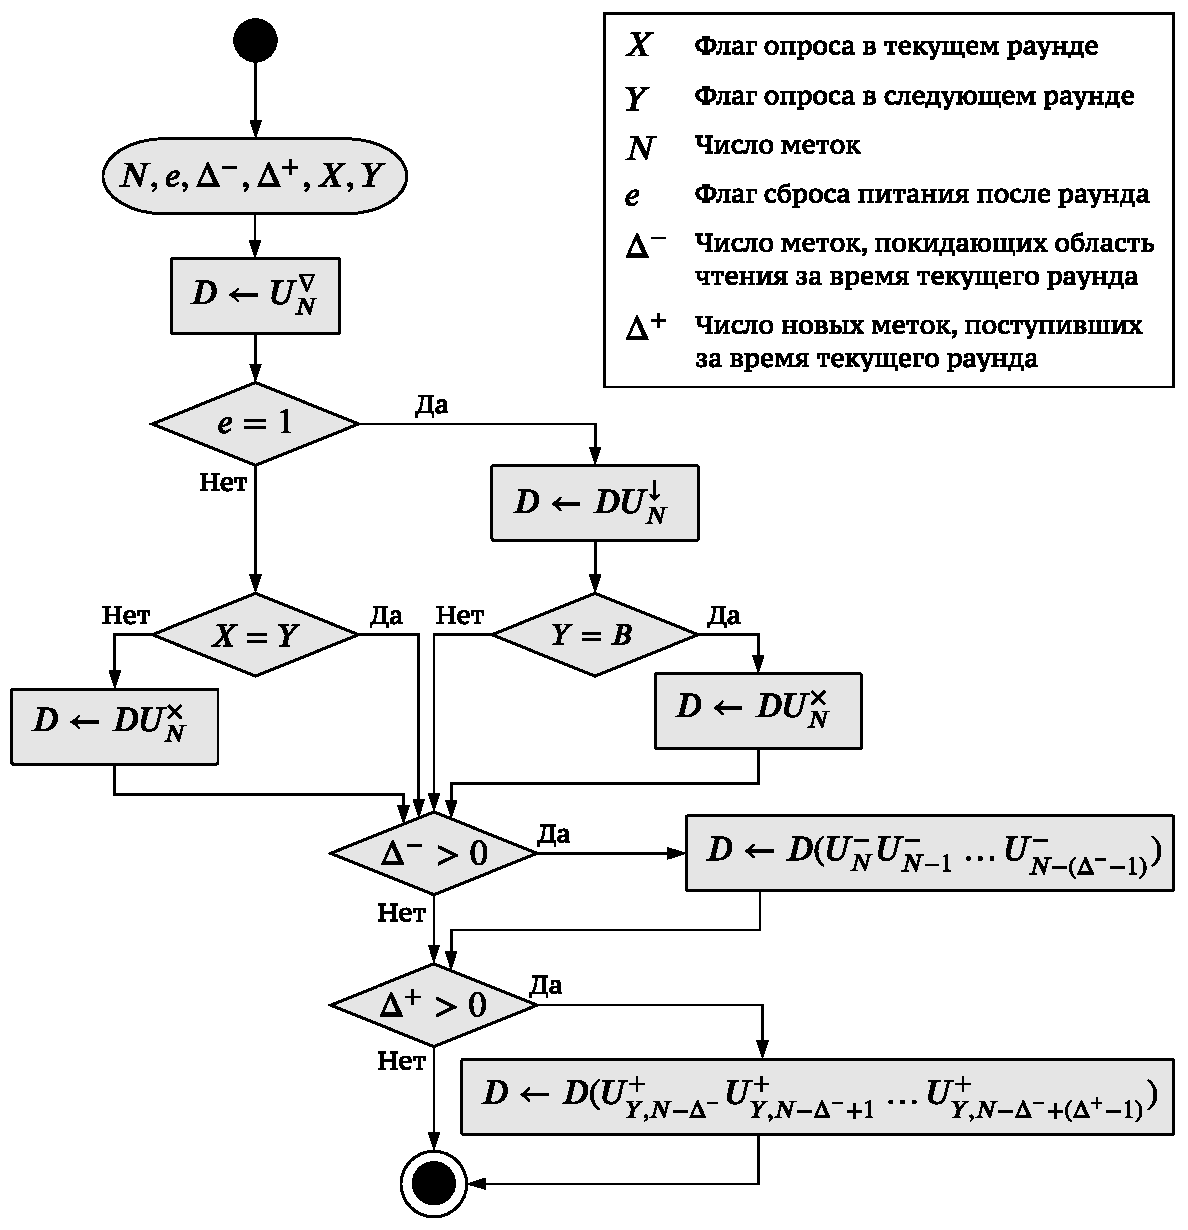
\includegraphics[width=0.65\textwidth]{chapter3/ch3_matrix_composition}
    \end{center}
\end{frame}

% \begin{center}
%   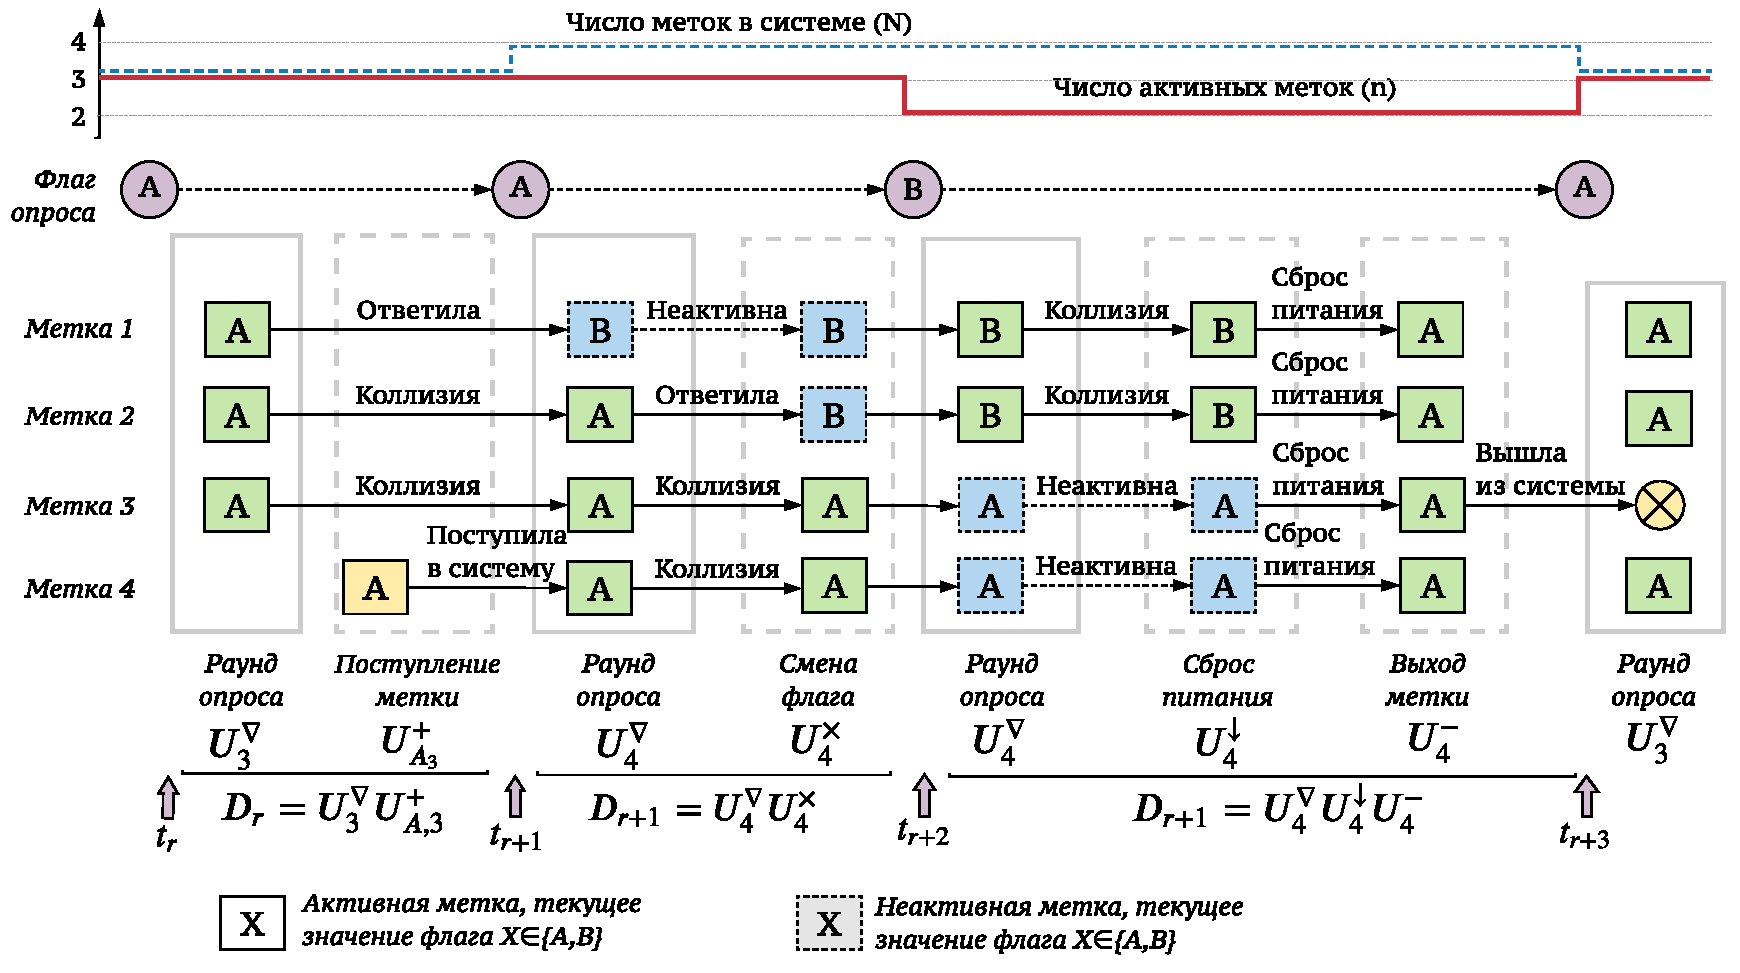
\includegraphics[width=0.8\textwidth]{chapter3/ch3_decomposition}
% \end{center}

\begin{frame}
    \frametitle{Элементарные операции в фоновом процессе}
    \begin{center}
        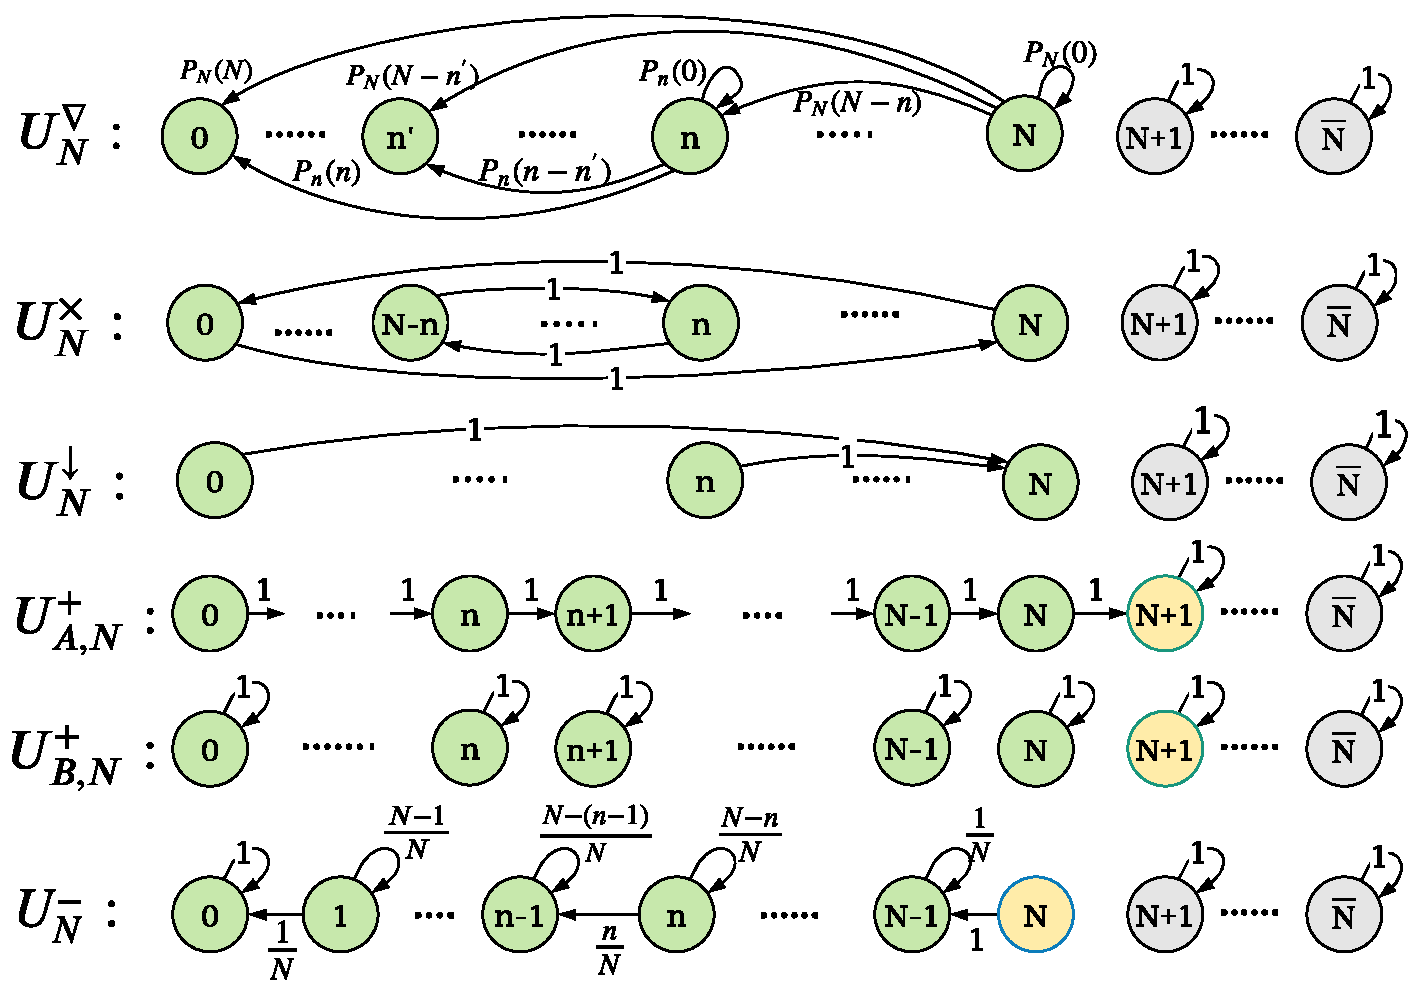
\includegraphics[width=0.75\textwidth]{chapter3/ch3_bg_trans.pdf}
    \end{center}

    \footnotesize
    \begin{itemize}
        \item Каждой элементарной операции ставится в соответствие стохастическая матрица, содержащая вероятности переходов фонового процесса $\{ \eta_r \}$.
        \item $\overline{N}$ "--- максимально возможное число меток в области чтения.
        \item $P_n(m)$ "--- вероятность того, что ровно $m$ меток из $n$ активных передадут EPCID (не обязательно успешно).
    \end{itemize}
\end{frame}

\begin{frame}
    \frametitle{Расчет распределения числа активных меток}
    \footnotesize
    \begin{itemize}
        \item Считыватель повторяет сценарий своей работы в цикле. Делается допущение о том, что аналогично повторяется и размеченный сценарий, то есть после раунда со спецификацией $\widetilde{\alpha}_{R}$ начинается раунд $\widetilde{\alpha}_1$.
        \item По размеченному сценарию с помощью алгоритма композиции элементарных операций вычисляются стохастические матрицы $D_1, D_2, \dots, D_R$, где матрица $D_r$ описывет переходные вероятности между раундами $r$ и $r  (\textbf{mod } R) + 1$.
        \item Для распределения вероятностей $\bm{p}^{(r)}$ процесса $\{ \eta_r \}$ перед $(r + R)$-м шагом выполняется соотношение $\bm{p}^{(r+R)} = \bm{p}^{(r)} D_r D_{r+1} \dots D_R D_1 \dots D_{r-1}$.
        \item Подпроцесс $\{ \eta_i^{[r]} \}_{i=0}^\infty$, $\eta_i^{[r]} = \eta_{r+Ri}$, является однородным марковским с матрицей переходных вероятностей $\widetilde{D}_r = D_r D_{r+1} \dots D_R D_1 \dots D_{r-1}$.
        \item Для всевозможных подпроцессов $\{ \eta_i^{[r]} \}$, $r = 1, 2, \dots, R$ можно вычислить стационарные вероятности $\bm{\pi}^{(r)}$. Вероятности $\bm{\pi}^{(1)}$ можно найти как решение системы:
        \begin{equation*}
            \begin{cases}
                \bm{\pi}^{(1)} \widetilde{D}_1 &= \bm{\pi}^{(1)},\\
                \sum\limits_{n=0}^{\overline{N}} \pi^{(1)}_n &= 1,
            \end{cases}
        \end{equation*}
        а вероятности $\bm{\pi}^{(r)}$, $r = \overline{2, R}$ можно вычислить как $\bm{\pi}^{(r)} = \bm{\pi}^{(r-1)} D_{r-1}$.
    \end{itemize}
\end{frame}

\begin{frame}
    \frametitle{Состояния основного процесса}
    \begin{center}
        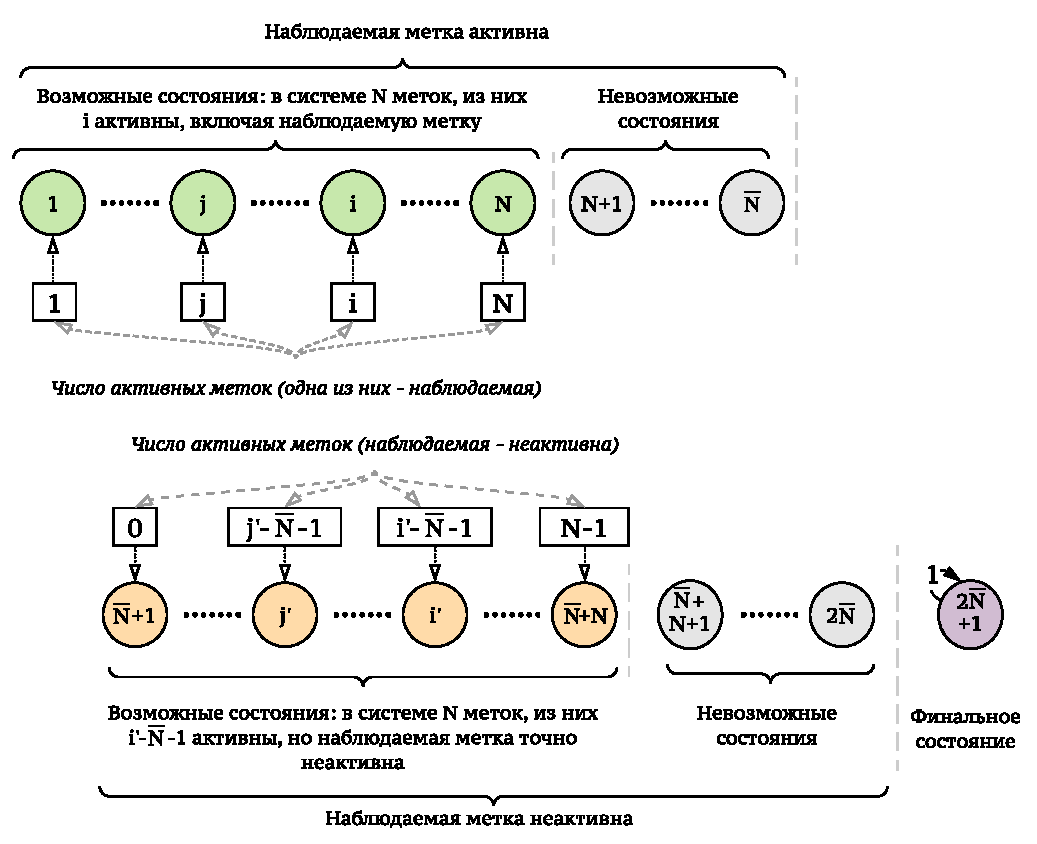
\includegraphics[width=0.9\textwidth]{chapter3/ch3_fg_structure}
    \end{center}

    \footnotesize
    Состояния основного процесса $\{(\eta_r, \phi_r)\}$ можно пронумеровать, чтобы получить одномерный процесс $\{ \gamma_r \}$:
    $$
        \begin{aligned}
            1 \leqslant \gamma_r \leqslant \overline{N}                 &\Leftrightarrow \phi_r = 1 \text{ и } \eta_r = \gamma_r; \\
            \overline{N} + 1 \leqslant \gamma_r \leqslant 2\overline{N} &\Leftrightarrow \phi_r = 0 \text{ и } \eta_r = \gamma_r - \overline{N} - 1;\\
            \gamma_r = 2\overline{N}+1                                  &\Leftrightarrow \phi_r = 2.
        \end{aligned}
    $$
    Состояние $\gamma_r = 2\overline{N} + 1$ является финальным (поглощающим).
\end{frame}

\begin{frame}[allowframebreaks]
    \frametitle{Матрицы операций основного процесса}
    \begin{center}
        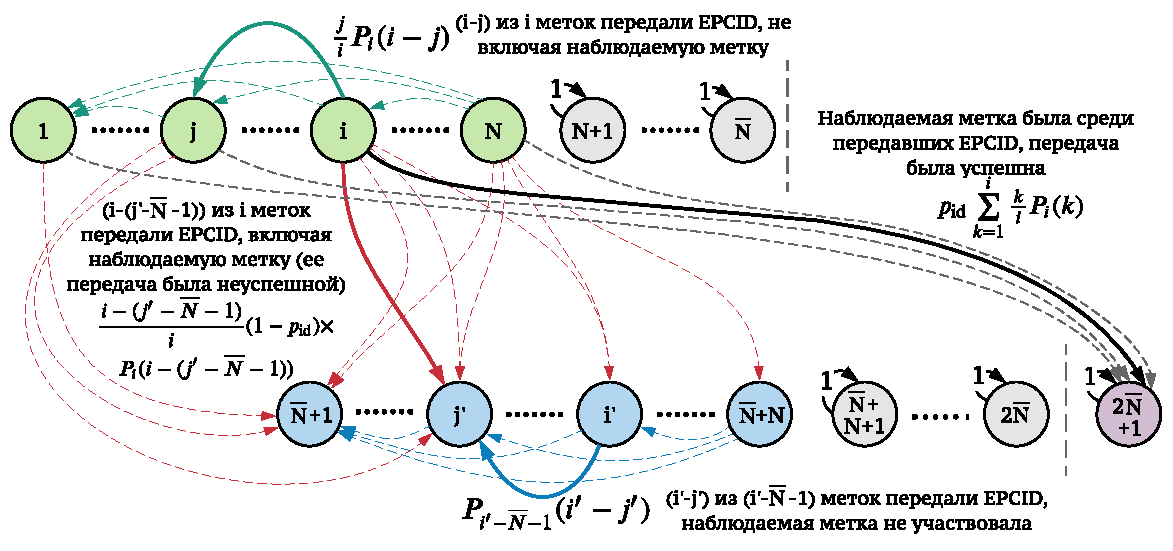
\includegraphics[width=1.0\textwidth]{chapter3/ch3_fg_trans_inventory}
    \end{center}
    \footnotesize
    \begin{itemize}
        \item Элементарным операциям можно поставить в соответствие стохастические матрицы $V^\nabla_N$, $V^\times_N$, $V^\downarrow_N$, $V^+_N$, $V^-_N$, содержащие вероятности переходов основного процесса $\{ \gamma_r \}$.
        \item На рисунке изображены переходы, соответствующие элементарной операции $V^\nabla_N$.
    \end{itemize}
    \vfill
    \framebreak
    \begin{center}
        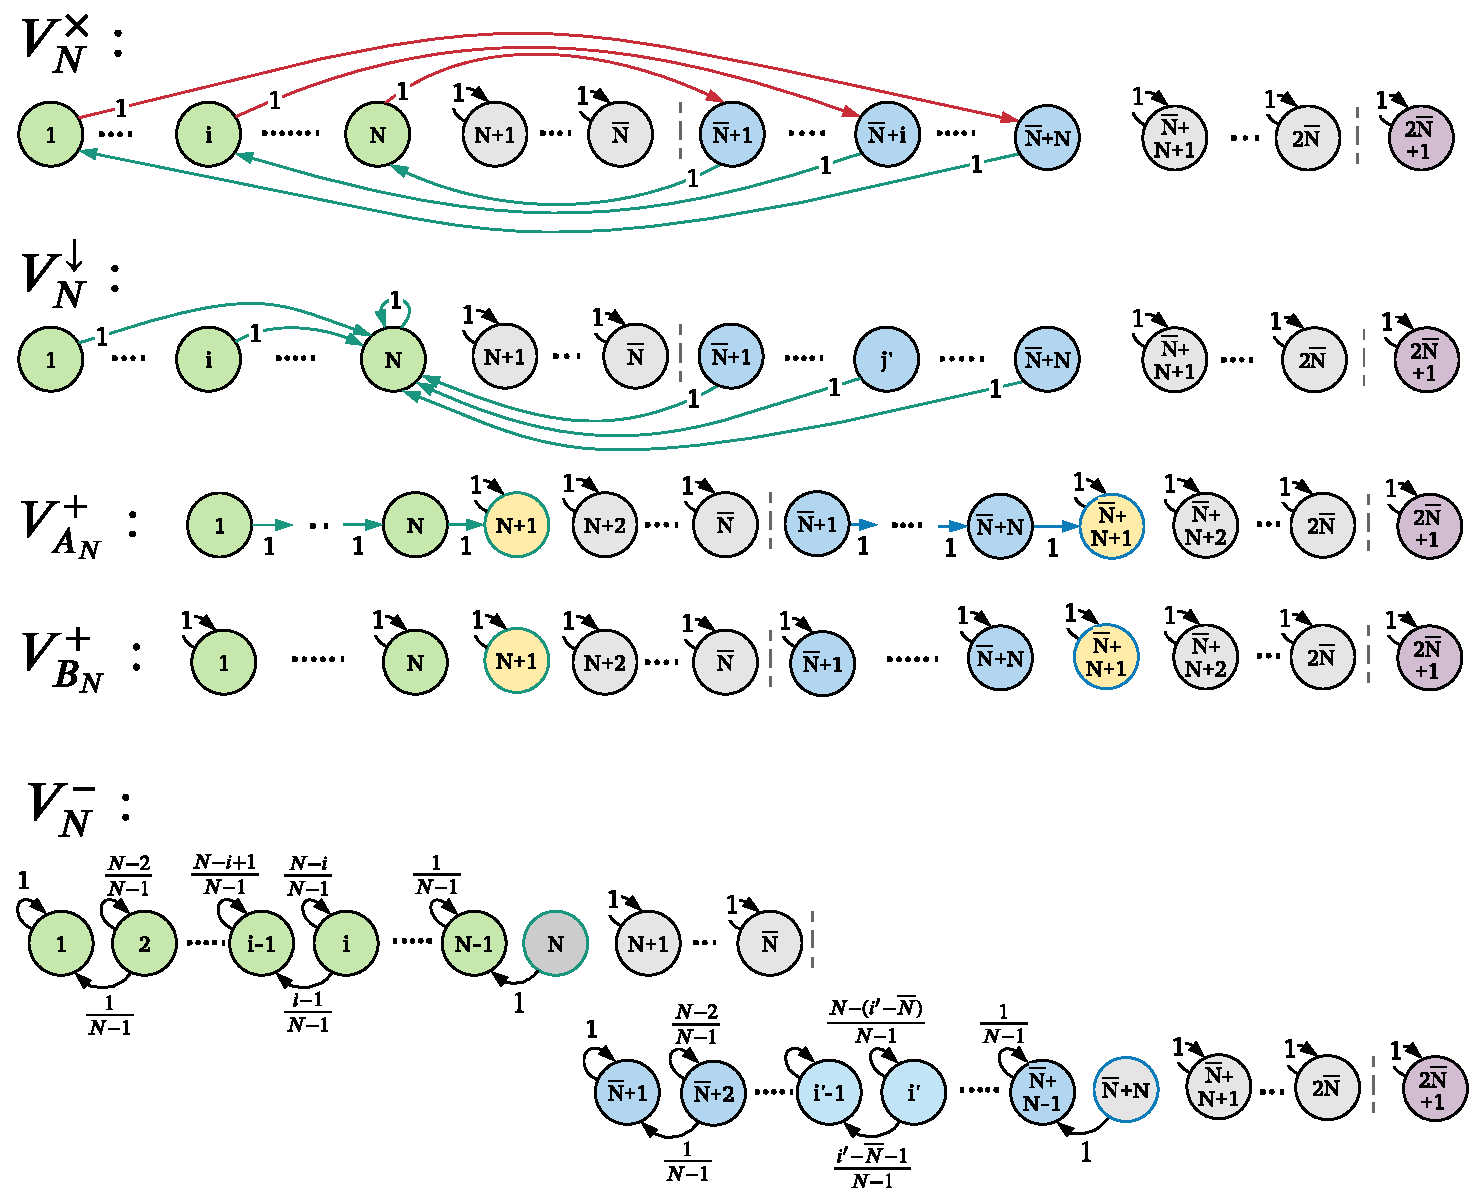
\includegraphics[width=1.0\textwidth]{chapter3/ch3_fg_trans}
    \end{center}
\end{frame}

\begin{frame}
    \frametitle{Вероятность поглощения основного процесса}
    \footnotesize
    \begin{itemize}
        \item Матрицы переходов $C_r^{[r_0]}$ основного процесса строятся из матриц элементарных операций с помощью алгоритма композиции, который использовался при построении матриц $D_r$.
        \item Наблюдаемая метка может поступить в любом из раундов $r_0$, перед которым в систему поступали метки, то есть $r_0 \in \mathfrak{R} = \{ r\:|\:r \in [1, R],\; \Delta_{r-1}^+ > 0 \}$.
        \item Пусть наблюдаемая метка поступила в систему в раунде $r_0$ и находится в системе в течение ровно $Q_{r_0}$ раундов. Обозначим $\bm{\theta}^{(r_0,r)} \in \mathbb{R}^{2\overline{N}+1}$ распределение вероятностей процесса $\gamma_r^{[r_0]}$ на $r$-м шаге, а $\bm{\theta}^{(r_0,1)}$ "--- его начальное распределение. Так как вероятности переходов между $r$-м и $(r+1)$-м раундами определяются матрицей $C_r^{[r_0]}$, то
        $$
        \bm{\theta}^{(r_0, Q_{r_0} + 1)} = \bm{\theta}^{(r_0, 1)} C^{[r_0]}_1 C^{[r_0]}_2 \cdots C^{[r_0]}_{Q_{r_0}}.
        $$
        \item В силу определения состояний процесса $\{ \gamma_r^{[r_0]} \}$, вероятность поглощения (идентификации наблюдаемой метки):
        $$
	        \mathbb{P}\{ \phi_{Q_{r_0}}^{[r_0]} = 2 \} \equiv \mathbb{P}\{ \gamma_{Q_{r_0}}^{[r_0]} = 2\overline{N}+1 \} = \theta_{2\overline{N}+1}^{(r_0, Q_{r_0}+1)}.
        $$
    \end{itemize}
\end{frame}

\begin{frame}
    \frametitle{Расчет вероятности идентификации метки}
    \footnotesize
    Для расчета вероятности идентификации метки, нужно найти распределение вероятностей поступления метки в $r_0$-м раунде, вычислить начальные распределения $\bm{\theta}^{(r_0, 1)}$ и найти математическое ожидание $\mathbb{P}\{ \phi_{Q_{r_0}}^{[r_0]} = 2 \}$, рассматривая ее как функцию случайной величины $r_0$.
    \begin{itemize}
        \item Вероятность поступления метки в $r_0$-м раунде:
        $$
            p^{[a]}_{r_0} = \frac{\tau_{r_0}}{\sum_{r \in \mathfrak{R}} \tau_r}
        $$
        \item Начальное распределение $\bm{\theta}^{(r_0, 1)}$ процесса $\gamma_r^{[r_0]}$ можно получить из распределения $\bm{\pi}$ фонового процесса $\{ \eta_r \}$:
        $$
            \theta_n^{(r_0,1)} = \begin{cases}
                \pi^{(r_0)}_n,                      &\widetilde{\alpha}_{r_0} = A^e_N,\; 1 \leqslant n \leqslant N\\
                \pi^{(r_0)}_{n - (\overline{N}+1)}, &\widetilde{\alpha}_{r_0} = B^e_N,\; \overline{N}+1 \leqslant n \leqslant \overline{N}+N\\
                0,                                  &\text{в остальных случаях.}
            \end{cases}
        $$
    \end{itemize}
    \footnotesize
    \begin{block}{Вероятность идентификации наблюдаемой метки}
        $$
        	P_X = \sum\limits_{r_0 \in \mathfrak{R}} p_{r_0}^{[a]} \{ \bm{\theta}^{(r_0,1)} C_1^{[r_0]} C_2^{[r_0]} \cdots C_{Q_{r_0}}^{[r_0]} \}_{2\overline{N}+1},
        $$
    \end{block}
\end{frame}

\begin{frame}
    \frametitle{Результаты: анализ свойств раундов}
    \begin{center}
        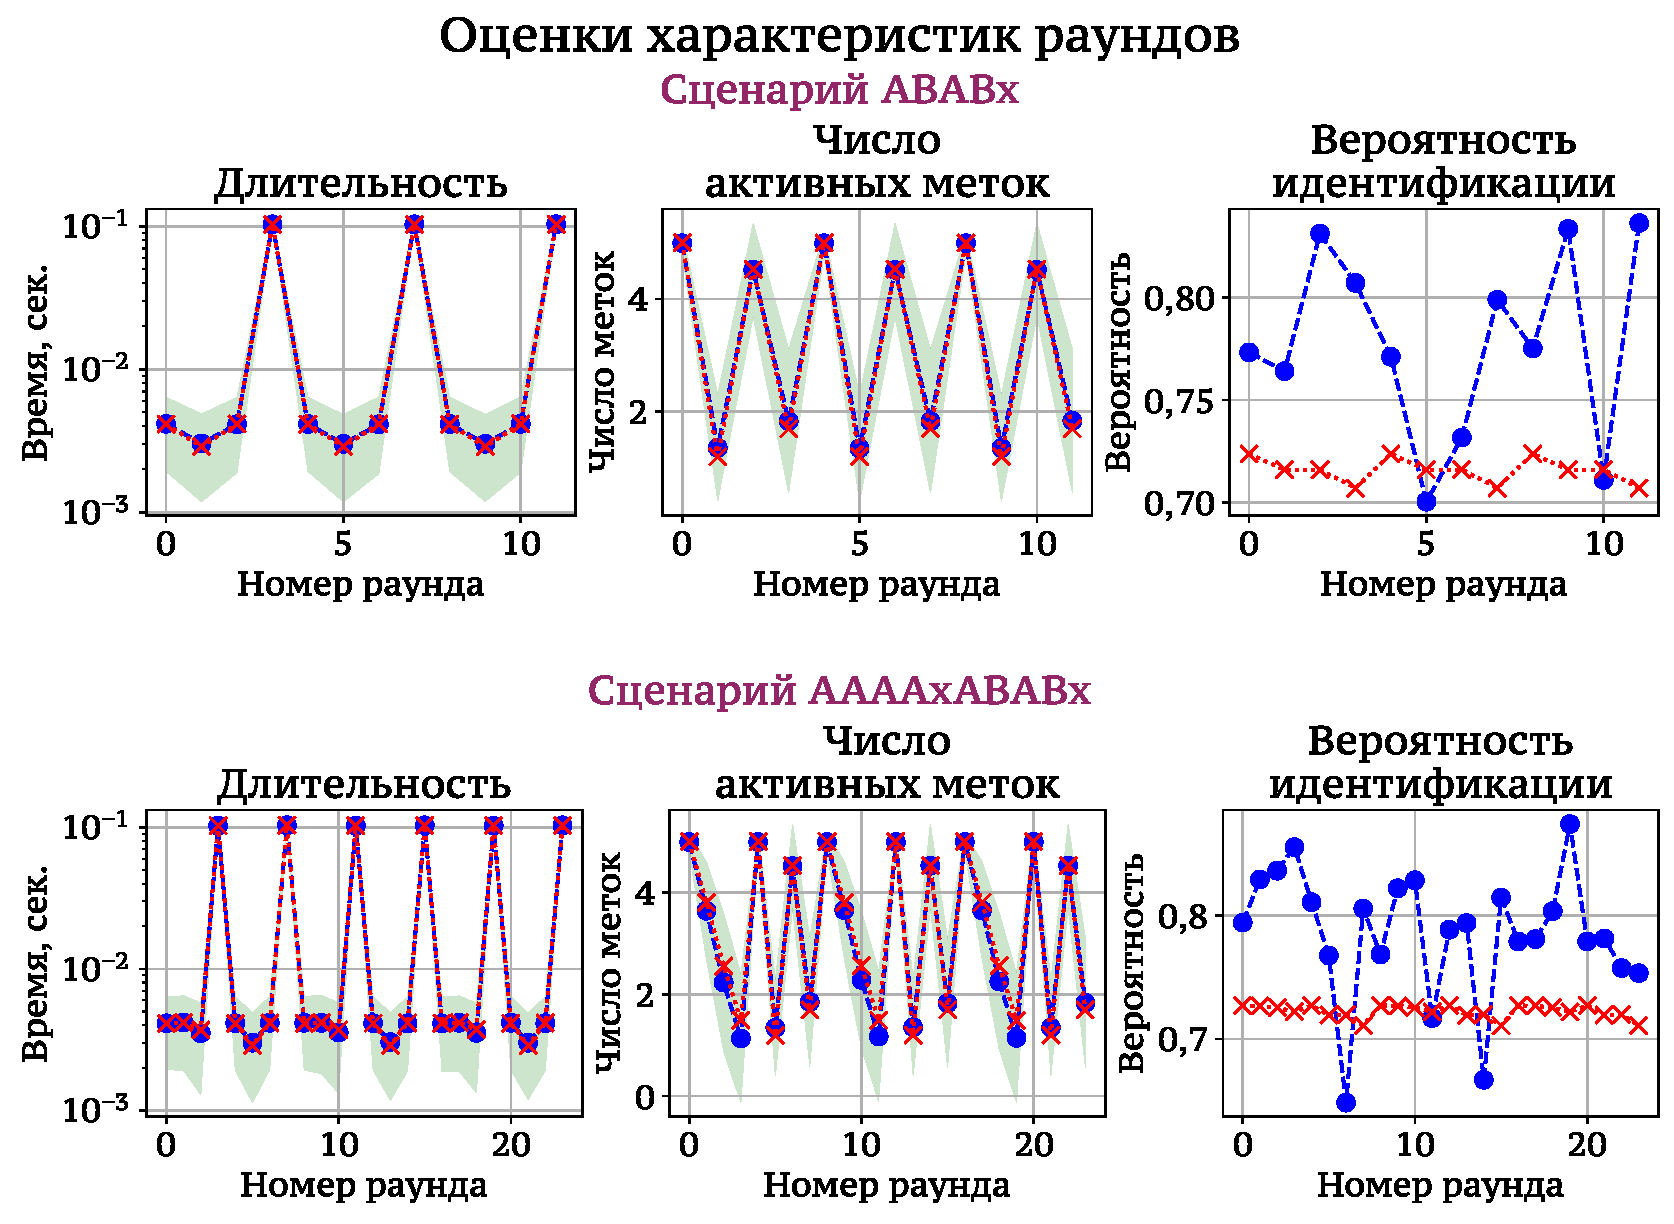
\includegraphics[width=0.75\textwidth]{chapter3/ch3_results_rounds_props}
    \end{center}
    \footnotesize
    \begin{itemize}
        \item Для валидации была разработана быстрая имитационная модель.
        \item Аналитический расчет был реализован на Python, имитационная модель "--- на Cython. Исходный код: \url{https://github.com/larioandr/thesis-rfidam}.
    \end{itemize}
\end{frame}

\begin{frame}
    \frametitle{Результаты: валидация модели}
    \begin{center}
        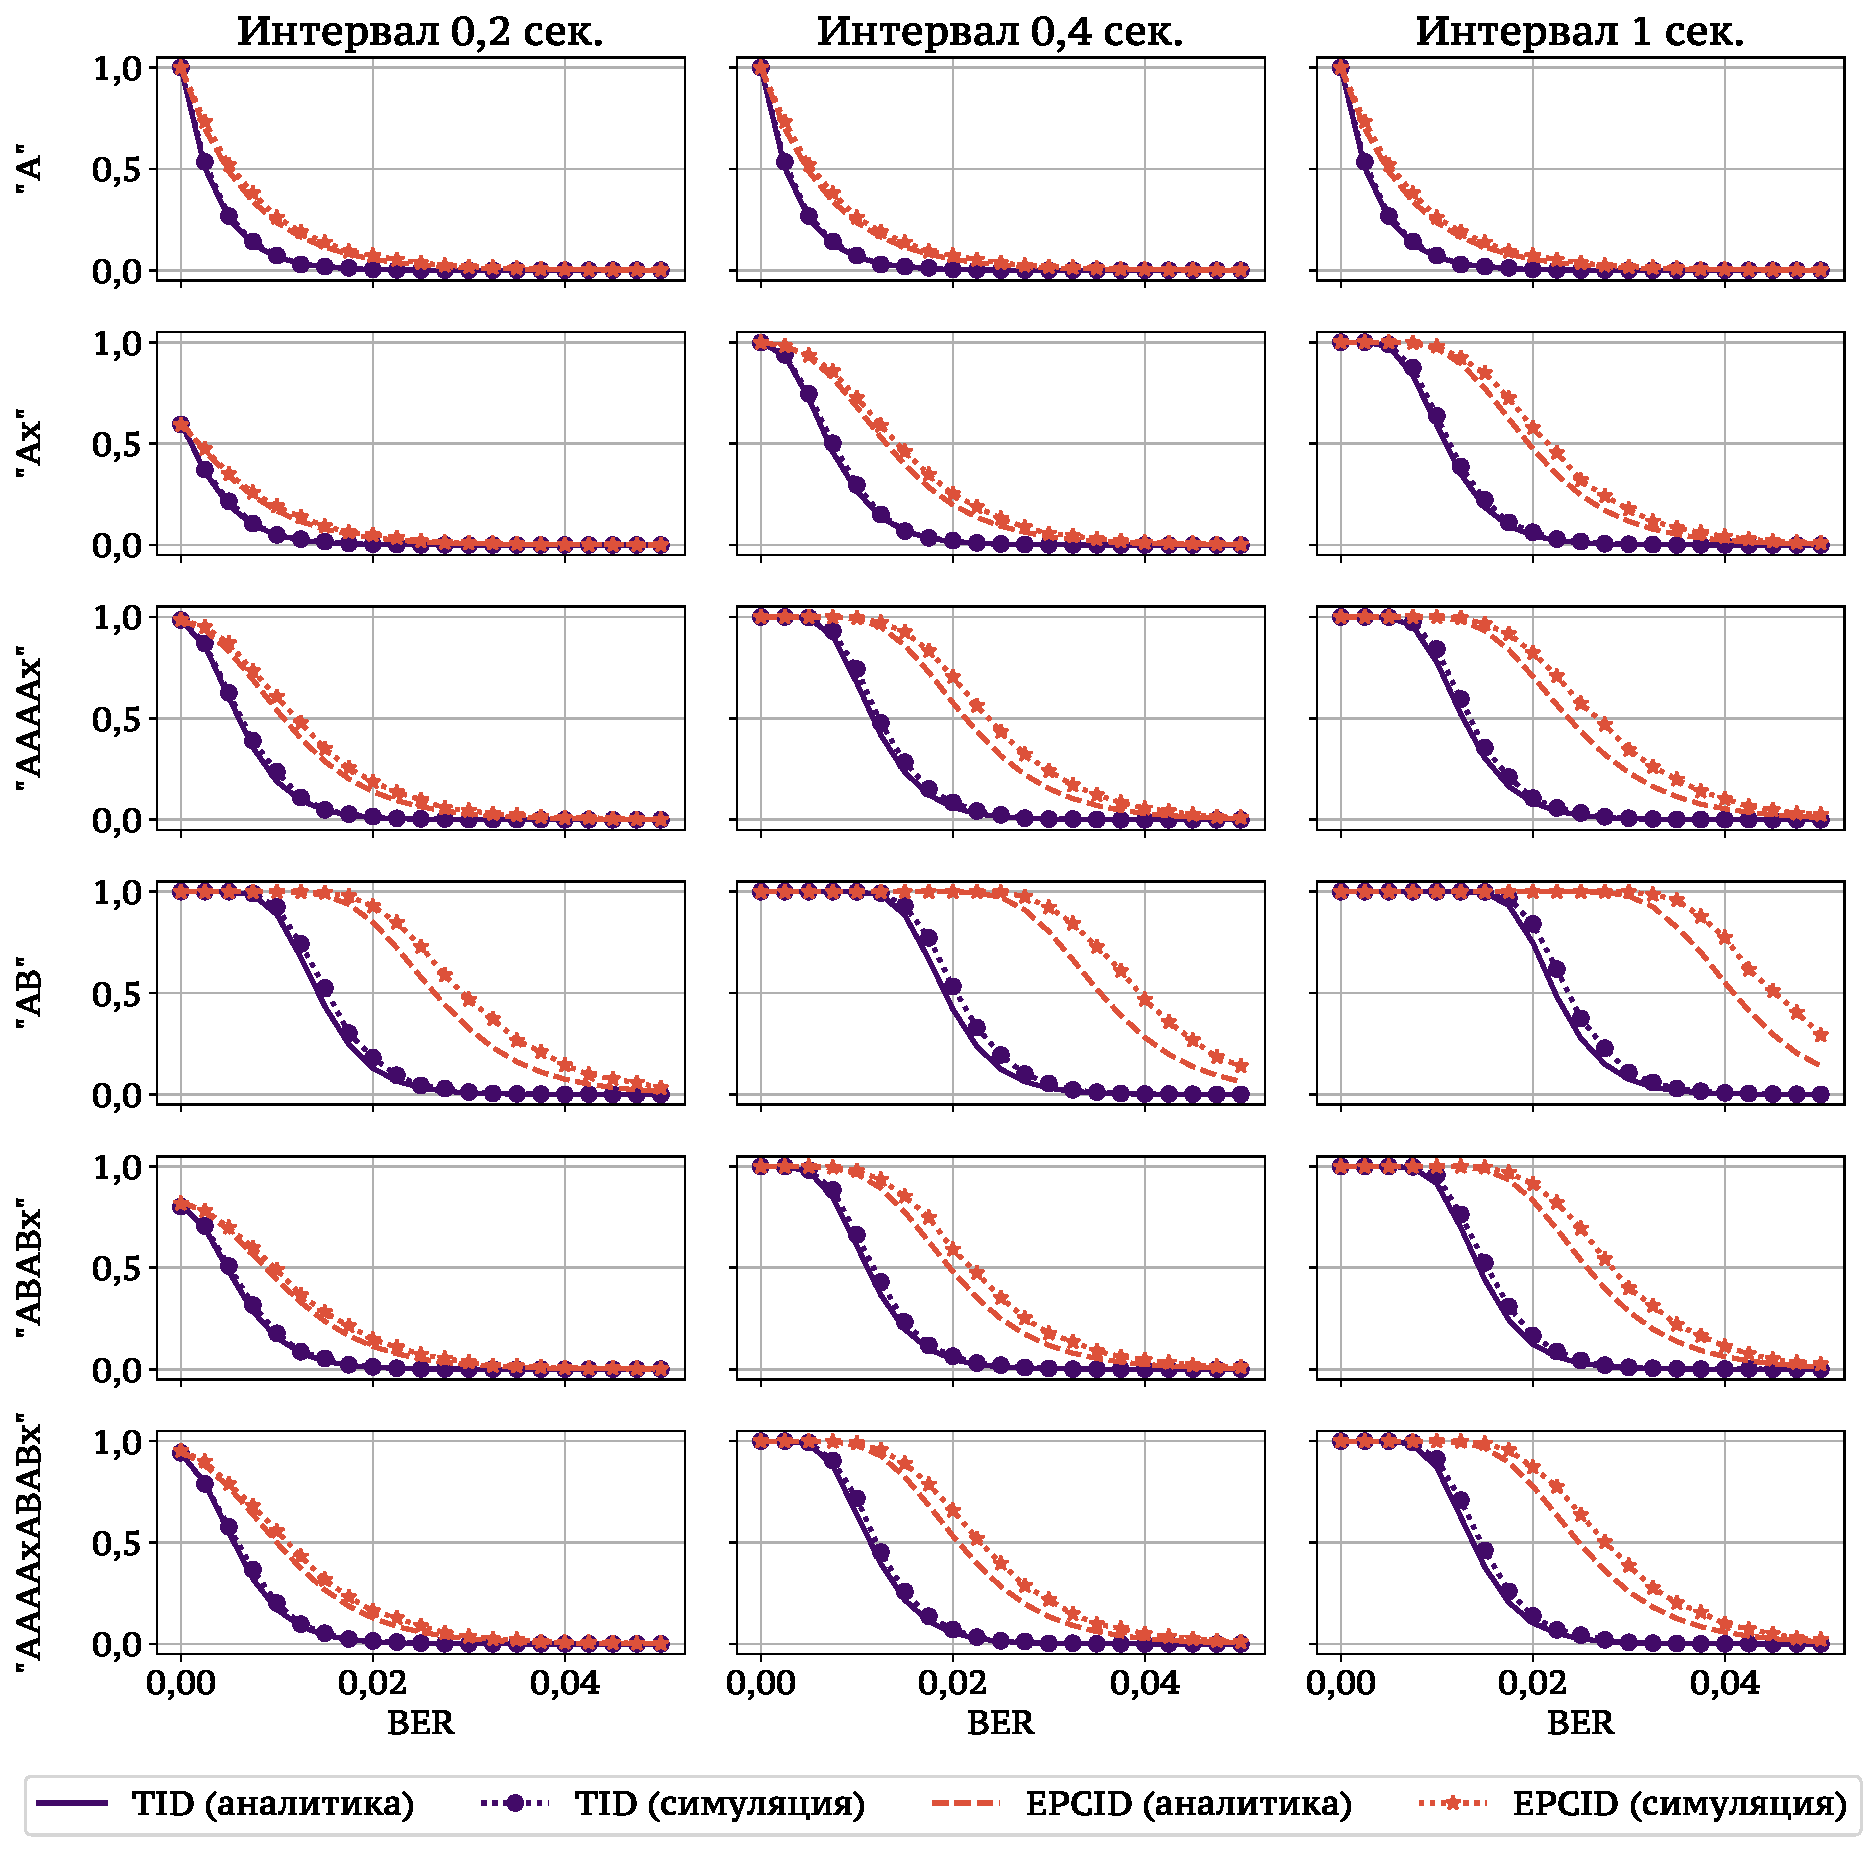
\includegraphics[width=0.83\textwidth]{chapter3/ch3_results_prob_cmp}
    \end{center}
\end{frame}

\begin{frame}
    \frametitle{Результаты: вероятность идентификации}
    \begin{center}
        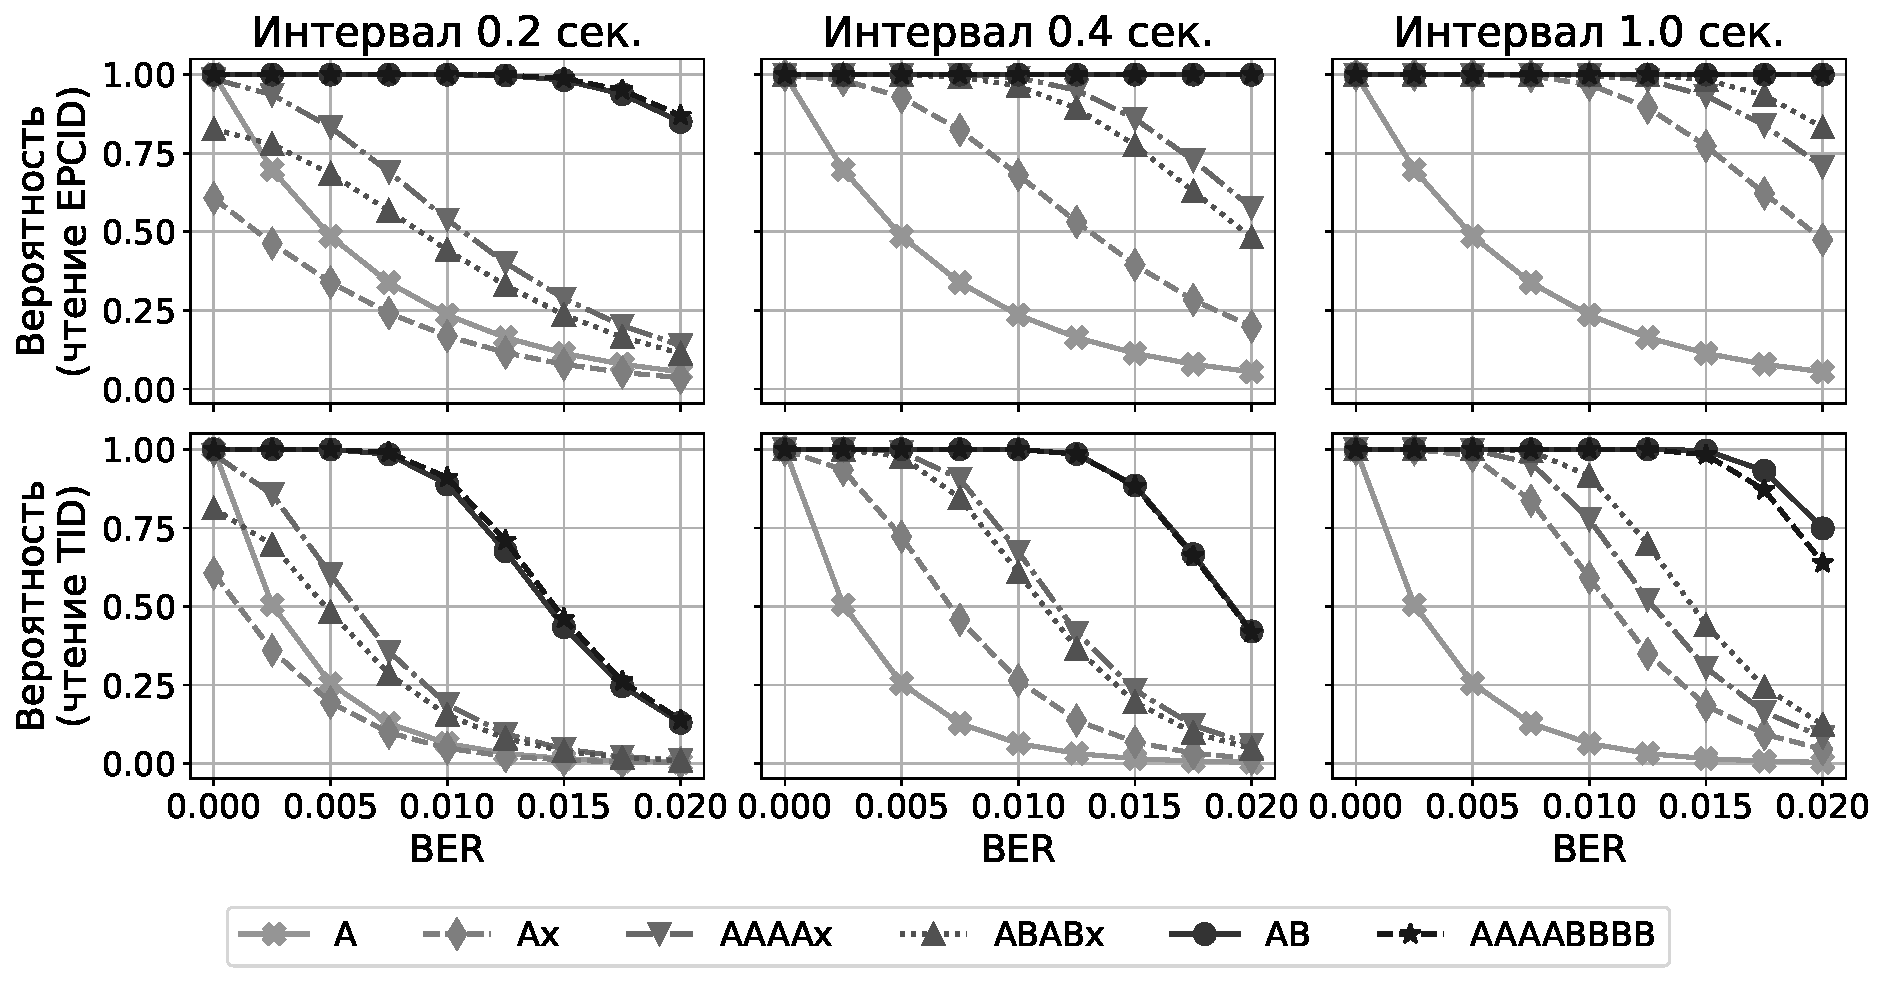
\includegraphics[width=0.9\textwidth]{chapter3/ch3_results_probs}
    \end{center}
    \vfill
    \begin{itemize}
        \item Чередование значений флагов сессий, по которым производится опрос, позволяет значительно повысить вероятность идентификации метки.
        \item Периодические отключения считывателя повышают вероятность идентификации в меньшей степени и эффективны только при малых значениях BER и больших интервалах между поступлениями меток в область чтения.
    \end{itemize}
\end{frame}

\begin{frame}
    \frametitle{Выводы}
    \footnotesize
    \begin{itemize}
        \item Предложена новая аналитическая модель системы радиочастотной идентификации мобильных меток, позволяющая учитывать сбросы питания считывателем и смены флагов сессий. Модель позволяет находить оценки длительностей раундов и вероятности идентификации меток. Модель включает в себя два неоднородных марковских процесса, описывающих число участвующих в каждом раунде меток, и состояние отдельной метки, для которой вычисляется вероятность идентификации.
        \item Приведены численные результаты, показывающие, что периодические смены флагов опросов значительно повышают вероятность идентификации движущейся метки. Сбросы питания также повышают вероятность, но менее эффективны.
        \item Приведены результаты сравнения аналитической и имитационной моделей, подтверждающие высокую точность аналитической модели.
        % \item Результаты были представлены и опубликованы в сборниках международных конференций IEEE RFID 2018 (США), ICAAP \& SP 2019 (Индия) и DCCN 2019 (Москва).
    \end{itemize}
\end{frame}





% ============================================================================
% ЧАСТЬ 4. АНАЛИЗ ПРОИЗВОДИТЕЛЬНОСТИ ОПОРНОЙ БЕСПРОВОДНОЙ СЕТИ
% ============================================================================
\section{Анализ производительности опорной беспроводной сети}
\begin{frame}[plain, noframenumbering]
    \begin{center}
        \Huge
        Анализ производительности опорной беспроводной сети
    \end{center}
\end{frame}

\begin{frame}
    \frametitle{Постановка задачи}
    \begin{center}
        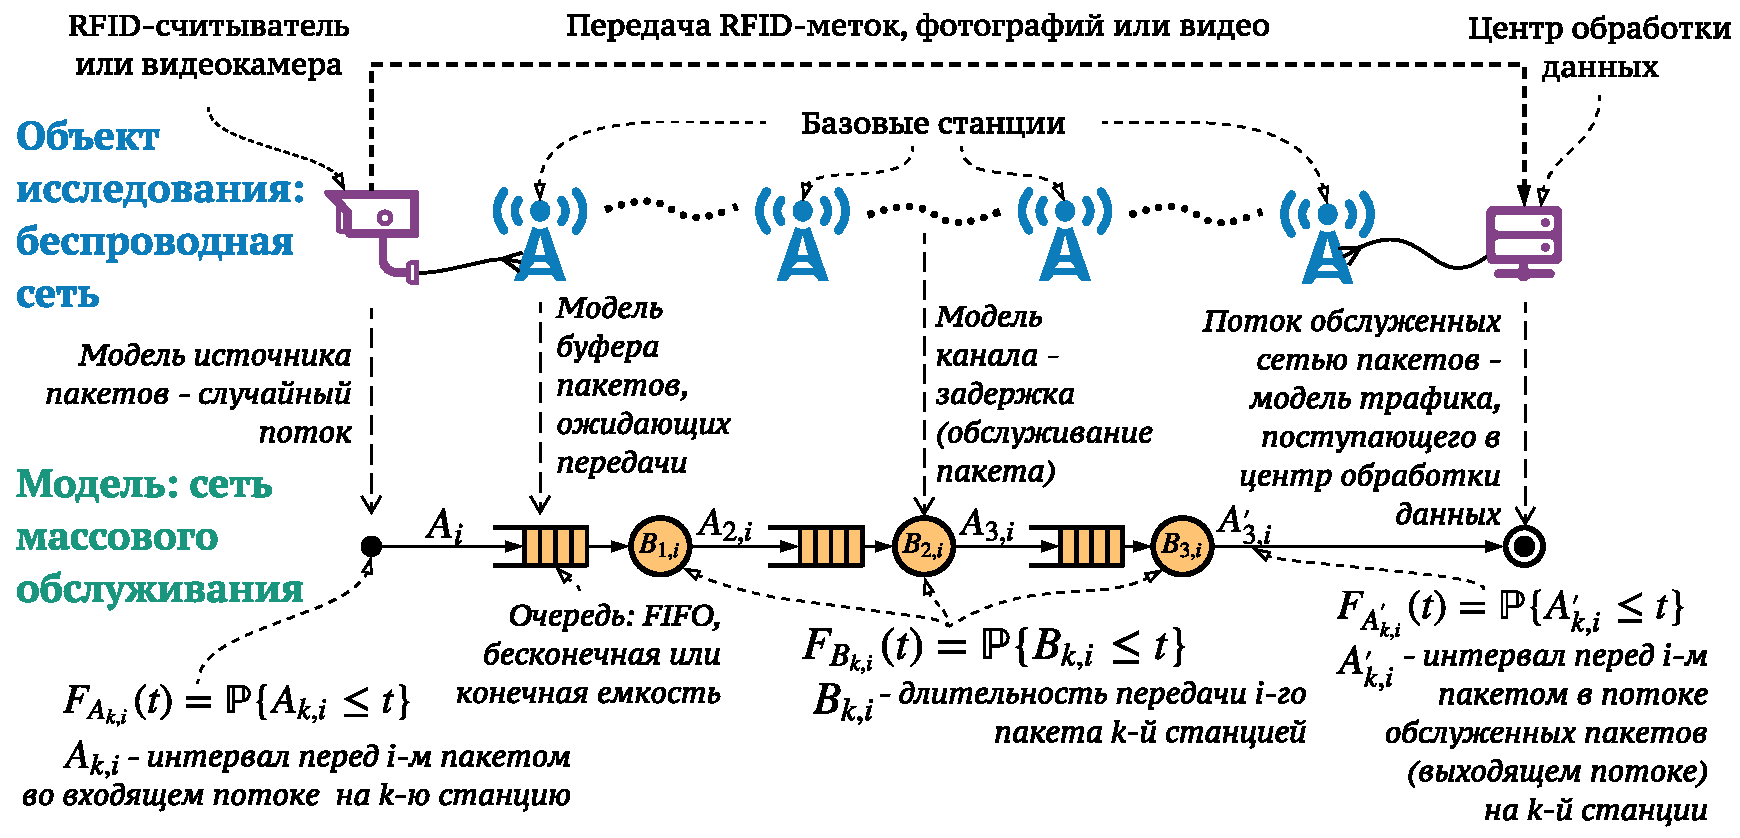
\includegraphics[width=1.0\textwidth]{chapter4/ch4_network_and_model}
    \end{center}
    \small
    \begin{alertblock}{Задача}
        Разработать методику оценки производительности широкополосных беспроводных сетей, использующихся для передачи данных от RFID-считывателей в центры обработки данных, на основе методов теории массового обслуживания и марковских случайных процессов.
    \end{alertblock}
\end{frame}

\begin{frame}
    \frametitle{Постановка задачи}
    Для решения задачи требовалось:
    \begin{itemize}
        \item Найти эффективный численный метод расчета характеристик тандемной сети массового обслуживания с коррелированными входящими потоками.
        \item Разработать методику выбора случайных распределений, адекватно моделирующих время передачи пакетов в беспроводных каналах.
    \end{itemize}
    \vfill
\end{frame}

\begin{frame}
    \frametitle{Система массового обслуживания MAP/PH/1/M}
    \small
    Для моделирования беспроводных каналов в диссертационном исследовании используются системы массового обслуживания с коррелированными входящими марковскими потоками и буфером ограниченной емкости MAP/PH/1/M.
    \footnotesize
    \begin{itemize}
        \item Входящий трафик моделируется с помощью MAP-потока $X \sim \text{MAP}(D_0, D_1)$, где матрицы $D_0, D_1$ удовлетворяют ограничениям:
        $$
            \begin{aligned}
                &\forall i: \sum\limits_{j=1} \{D\}_{ij} = 0, \quad
                \forall i \neq j: \{D\}_{ij} \geq 0, \quad
                \forall i: \{D\}_{ii} \leq 0,\\
                &\forall i, j: \{D_{1}\}_{ij} \geq 0,\quad
                \forall i \neq j: \{D_{0}\}_{ij} \geq 0, \quad
                \forall i: \{D_{0}\}_{ii} \leq 0.
            \end{aligned}
        $$
        \item Время обслуживания имеет распределение фазового типа (PH) $Y \sim \text{PH}(S, \bm{\tau})$, где:
        $$
            \begin{aligned}
                &\tilde{S} = \begin{bmatrix}
                S  & -S\mathbf{1} \\
                \mathbf{0} &  0
                \end{bmatrix} \mbox{"--- инфинитезимальная матрица,}\\
                &\forall i = \overline{1,V}: \: 0 \leq \tau_i \leq 1, \qquad
                \sum\limits_{i=1}^{V} \tau_i = 1.
            \end{aligned}
        $$
        \item $M$ "--- емкость буфера (очереди). Если входящий пакет застает очередь заполненной, он безвозвратно теряется.
    \end{itemize}
\end{frame}

\begin{frame}
    \frametitle{Основные свойства системы MAP/PH/1/M}
    \footnotesize
    Обозначим $W$ "--- порядок урпавляющей цепи MAP-потока, $V$ "--- порядок PH-распределения.
    Система MAP/PH/1/M обладает известными свойствами:
    \begin{itemize}
        \item Выходящий поток (обслуженных пакетов) из системы MAP/PH/1/M "--- MAP-поток $Z \sim \text{MAP}(D'_0, D'_1)$.
        \item Композиция MAP-потоков является MAP-потоком.
        \item Пусть $\overline{\psi}_{M+1}$ "--- распределение вероятностей состояний MAP-потока при полностью заполненной системе, $\lambda_X$ "--- интенсивность входящего MAP-потока $X \sim \text{MAP}(D_0, D_1)$, а $\bm{\theta}$ "--- распределение вероятностей управляющей цепи с генератором $D' = D'_0 + D'_1$. Тогда среднее число пакетов в системе $m_1$, вероятность потери пакета $P_L$ и длительность нахождения пакета в системе $T$ можно определить как:
        $$
            \begin{aligned}
            P_L &= \overline{\psi}_{M+1} \frac{D_1}{\lambda_X} \overline{\bm{1}},  \qquad T = \frac{m_1}{(1 - P_L)\lambda_X},\\
            m_1 &= \sum\limits_{k=0}^{M+1} \sum_{j=1}^{VW} k\theta_{kVW+j}.
            \end{aligned}
        $$
        \item{Порядок MAP-потока $Z$ обслуженных пакетов $U = (M+2)VW$.}
    \end{itemize}
\end{frame}

\begin{frame}
    \frametitle{Тандемная сеть с узлами MAP/PH/1/M}
    \begin{center}
        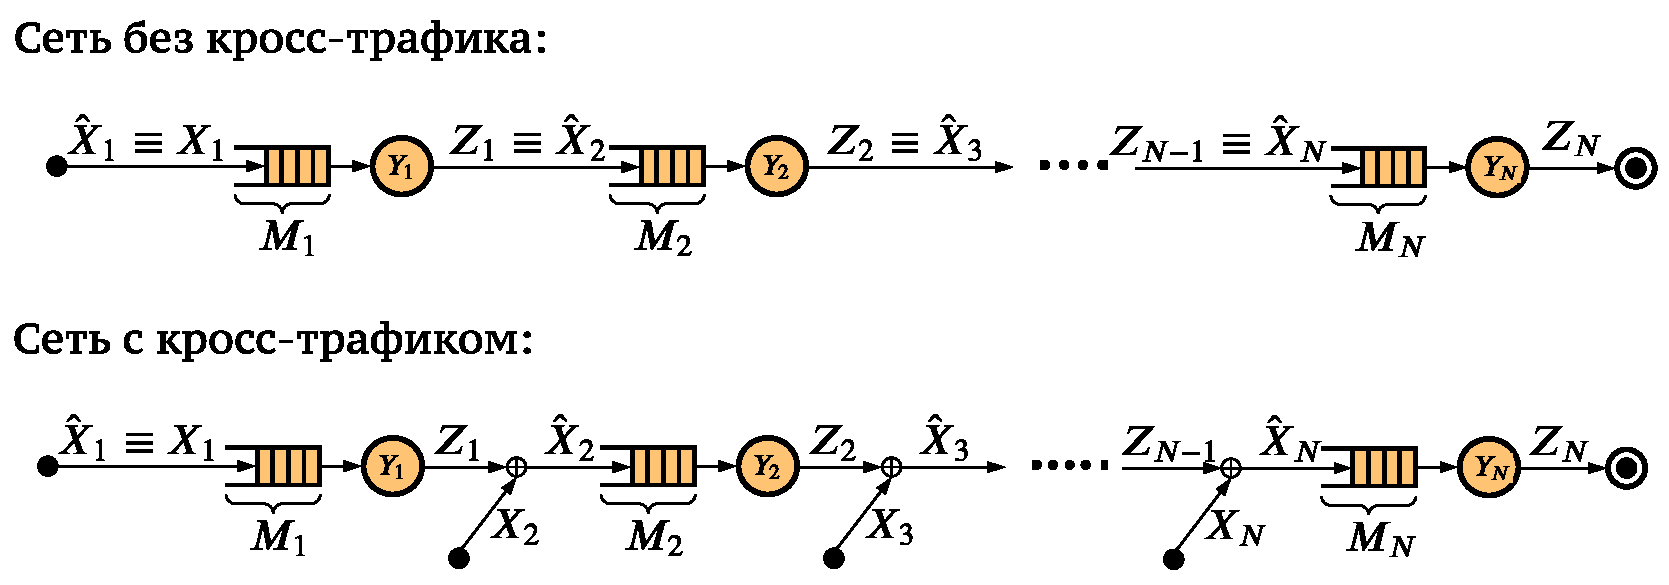
\includegraphics[width=1.0\textwidth]{chapter4/ch4_queueing_networks}
    \end{center}
    \footnotesize
    Благодаря тому, что композиция MAP-потоков является MAP-потоком, а также тому, что выходящий поток из системы MAP/PH/1/M является MAP-потоком, характеристики тандемной сети можно вычислить итерационно.

    \begin{exampleblock}{Утверждение}
        Пусть входящие MAP-потоки имеют порядок $W$, PH-распределения "--- порядок $V$, емкость очередей равна $M$, и сеть содержит $N$ станций. Тогда итерационная схема расчета характеристик тандемной сети имеет сложность:
        \begin{itemize}
            \item $O((M V W)^{3N})$, если в сети есть кросс-трафик;
            \item $O(W^3 (M V)^{3N})$, если кросс-тррафика в сети нет.
        \end{itemize}
    \end{exampleblock}
\end{frame}

\begin{frame}
    \frametitle{Расчет оценок характеристик СеМО}
    \footnotesize
    \begin{itemize}
        \item Точный расчет с помощью итерационного алгоритма: возможен только для сетей небольшой размерности (порядок выходящего потока с последней фазы $U_n \leqslant 8000$).
        \item {Расчет методом Монте-Карло
        \footnotesize
        \begin{itemize}
            \item \footnotesize Реализация метода "--- дискретно-событийная модель, реализована на C++/Cython.
            \item Точность определяется числом моделируемых событий появления новых пакетов
        \end{itemize}}
        \item {Расчет оценок характеристик методом понижения размерности потоков. В диссертационном исследовании рассматриваются аппроксимации:
        \footnotesize
        \begin{itemize}
            \item \footnotesize Выходящих с каждой фазы потоков.
            \item Входящих на каждую фазу потоков (включая входящий в сеть поток).
        \end{itemize}
        Для аппроксимации используется четыре варианта метода моментов:
        \begin{itemize}
            \item \footnotesize Аппроксимация по среднему интервалу $m_1$ пуассоновским потоком.
            \item Аппроксимация по $m_1$ и коэффициенту вариации $c_v$ гиперэкспоненциальными распределениями ($c_v > 1$), экспоненциальными распределениями ($c_v = 1$) или распределениями Эрланга ($c_v < 1$).
            \item Аппроксимация по $m_1$, $c_v$ и коэффициенту асимметрии $\gamma$ PH-распределениями.
            \item Аппроксимация по $m_1$, $c_v$, $\gamma$ и коэффициенту корреляции $\rho_1$ MAP-потоком.
        \end{itemize}}
    \end{itemize}
\end{frame}

\begin{frame}
    \frametitle{Случайный набор СеМО для численного эксперимента}
    \begin{columns}
        \begin{column}{0.65\linewidth}
            \begin{center}
                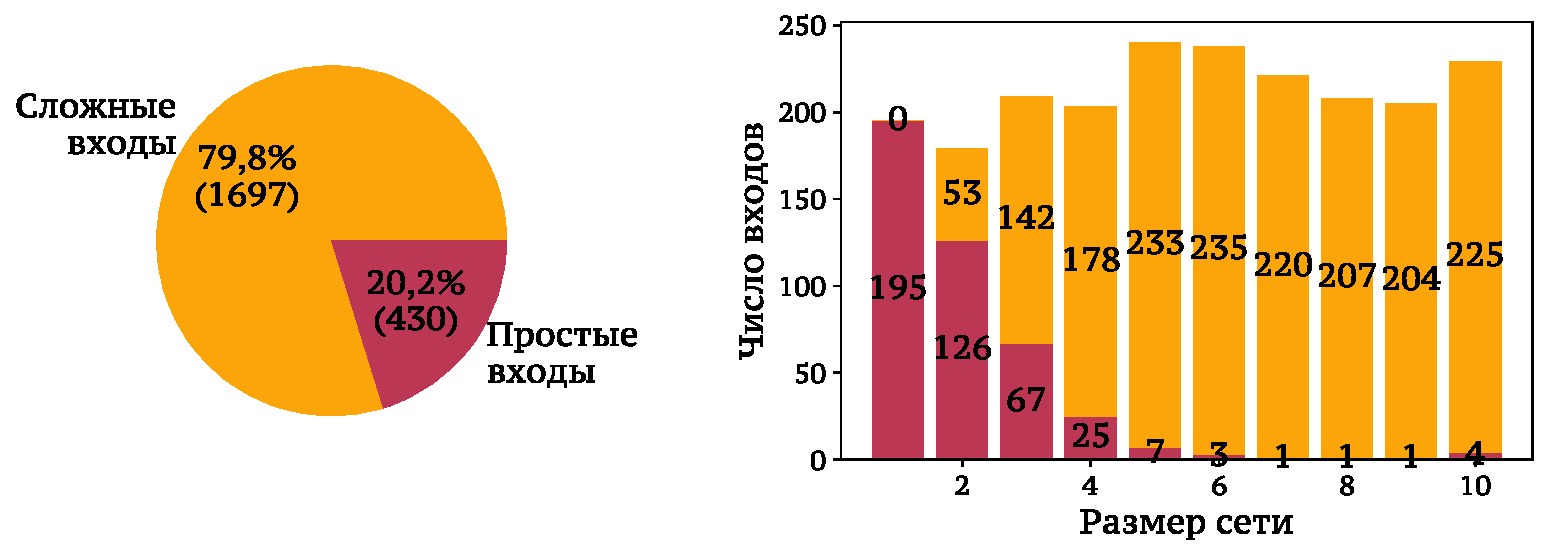
\includegraphics[width=\textwidth]{chapter4/ch4_complexity_split.pdf}
                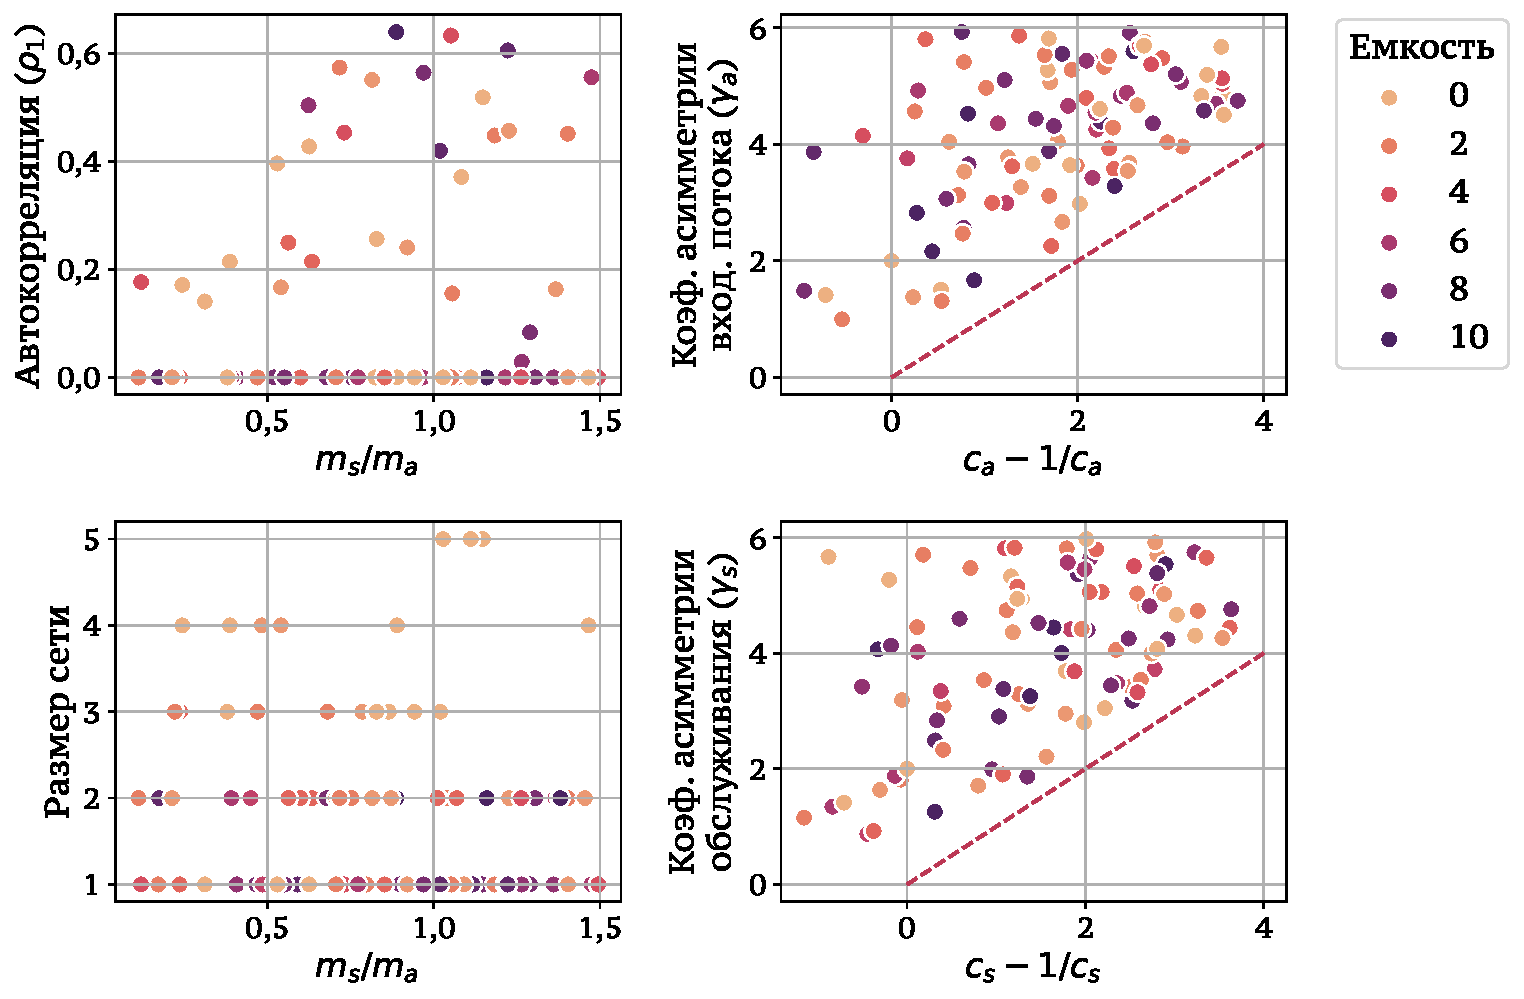
\includegraphics[width=\textwidth]{chapter4/ch4_input_scatter}
            \end{center}
        \end{column}
        \hfill
        \begin{column}{0.33\linewidth}
            \footnotesize
            \begin{itemize}
                \item Для численного эксперимента были случайно сгенерированы 2500 случайных СеМО (входной набор).
                \item С помощью алгоритма Тарьяна были отсеяны 373 СеМО, в которых цепи имели невозвратные состояния или распадались на сильно связанные компоненты.
            \end{itemize}
            \vfill
        \end{column}
    \end{columns}
\end{frame}

\begin{frame}
    \frametitle{Сравнение точности методов аппроксимации}
    \begin{columns}
        \begin{column}{0.55\linewidth}
            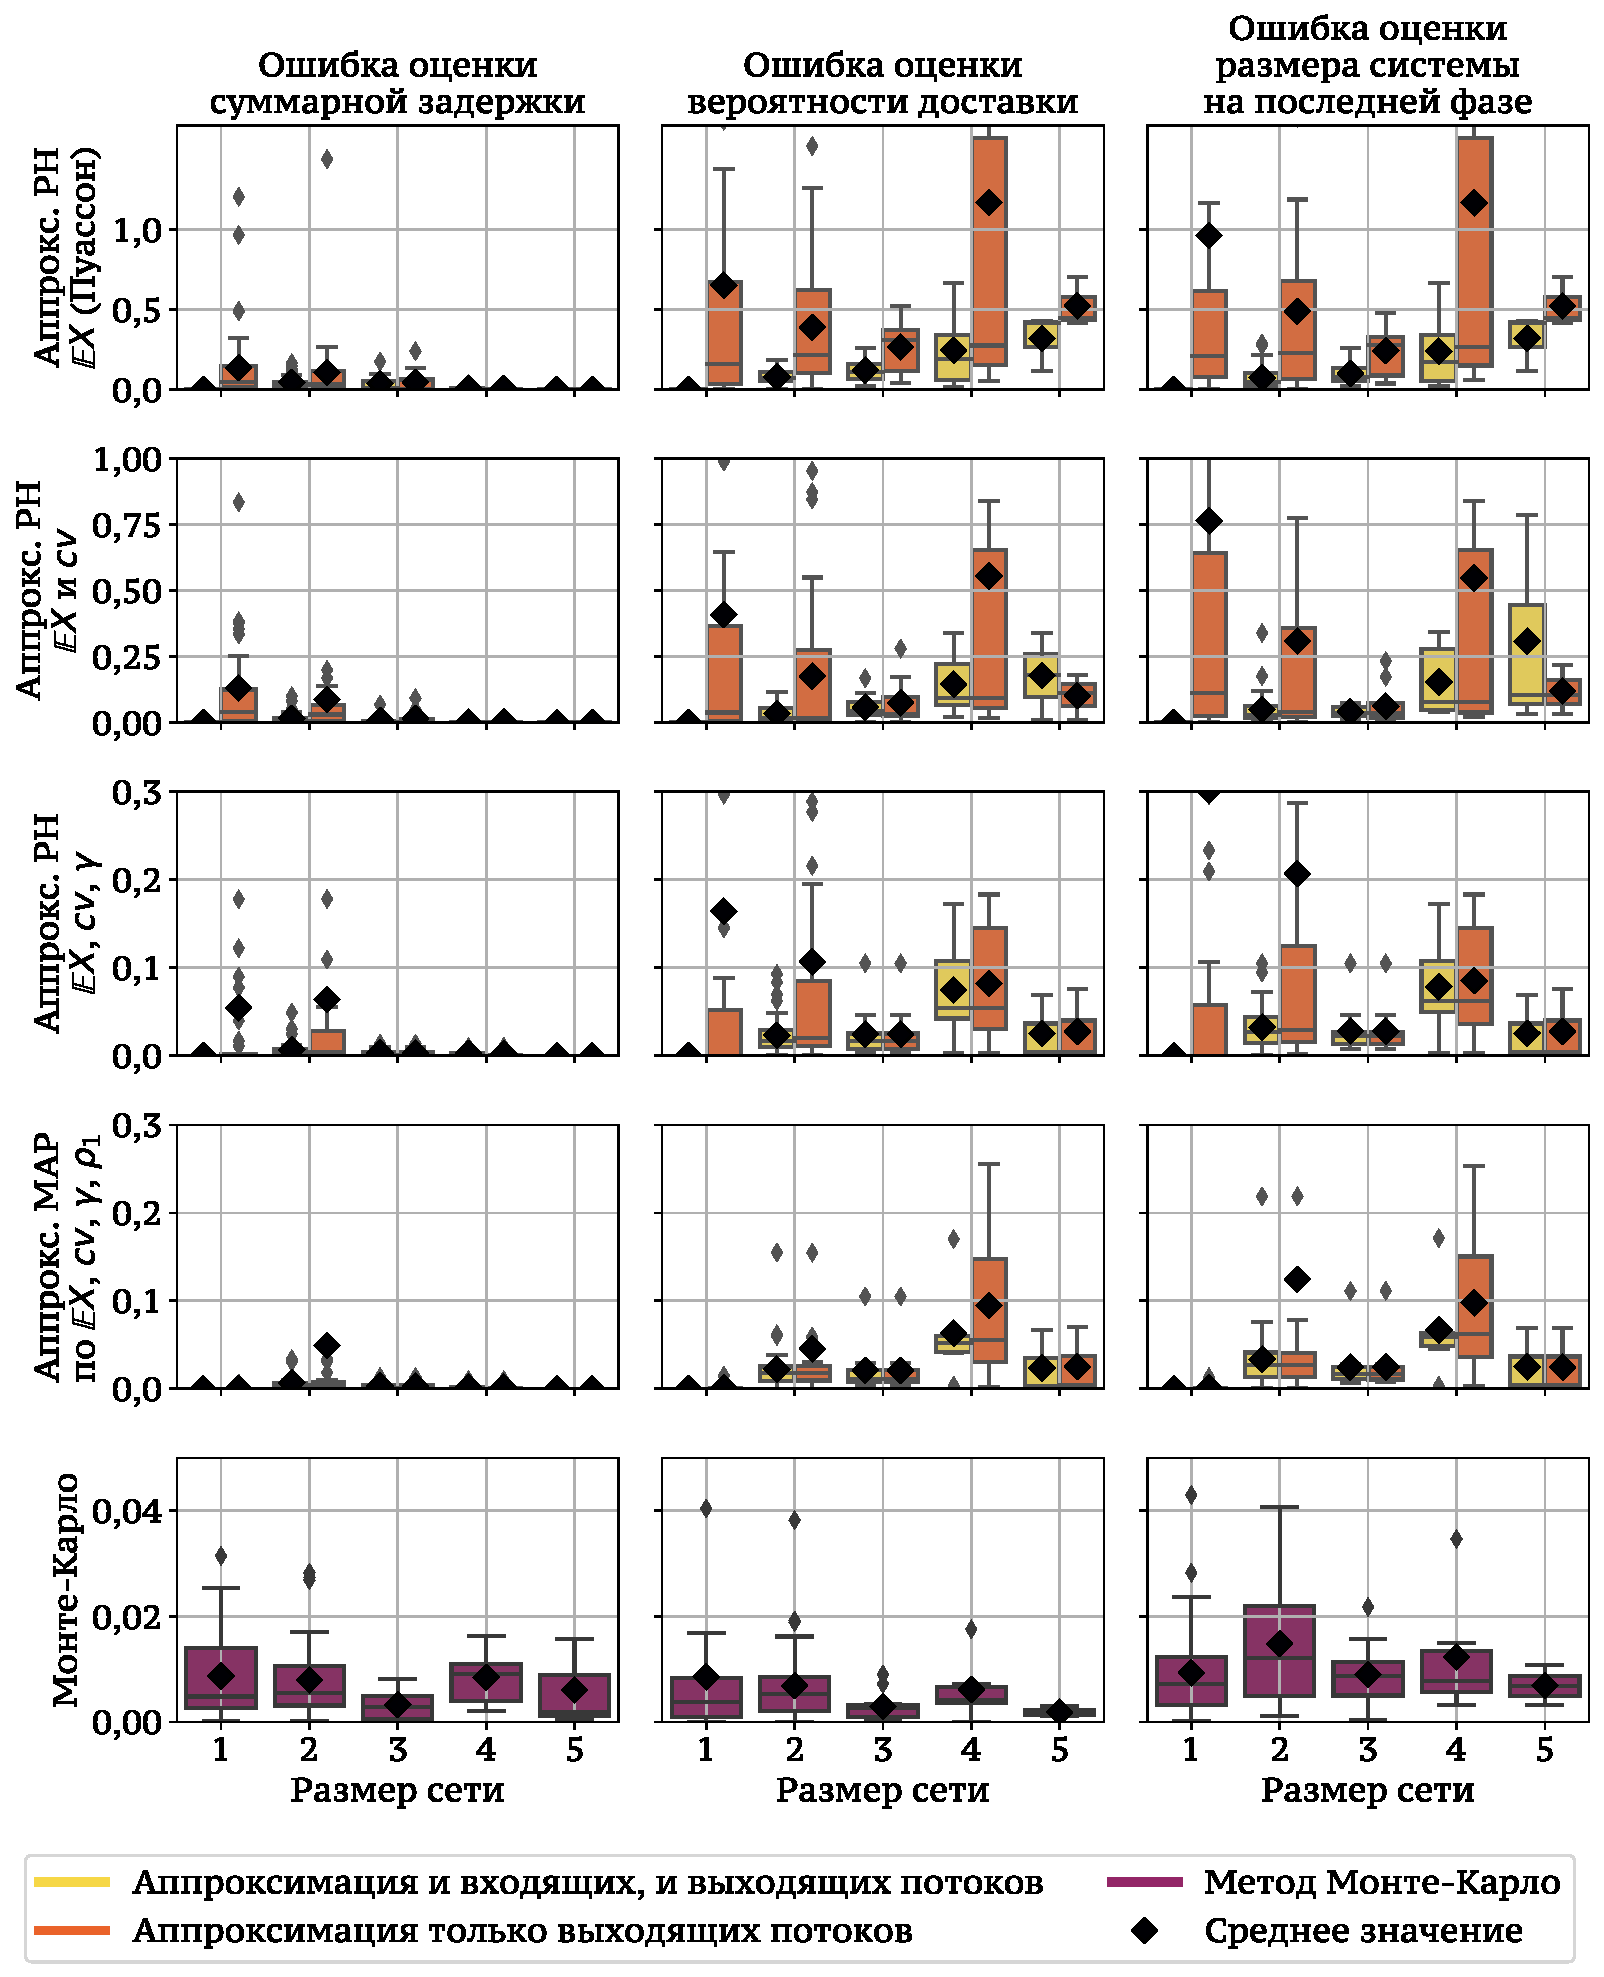
\includegraphics[width=\textwidth]{chapter4/ch4_approximations_summary}
        \end{column}
        \begin{column}{0.43\linewidth}
            \footnotesize
            \begin{itemize}
                \item Метод Монте-Карло обеспечивает самую высокую точность (свыше 0,98).
                \item Точность аппроксимации входящих потоков по трем моментам и коэффициенту корреляции $\sim$ 0,9.
                \item Точность аппроксимации выходящих потоков PH-распределениями по трем моментам $\sim$ 0,9.
                \item Точность аппроксиации по двум моментам выходящих потоков $\sim$ 0,8.
                \item Игнорирование коэффициента корреляции входящего потока ведет к ошибке оценки вероятности доставки и размера системы.
            \end{itemize}
        \end{column}
    \end{columns}
\end{frame}

\begin{frame}
    \frametitle{Сравнение длительности расчетов}
    \begin{center}
        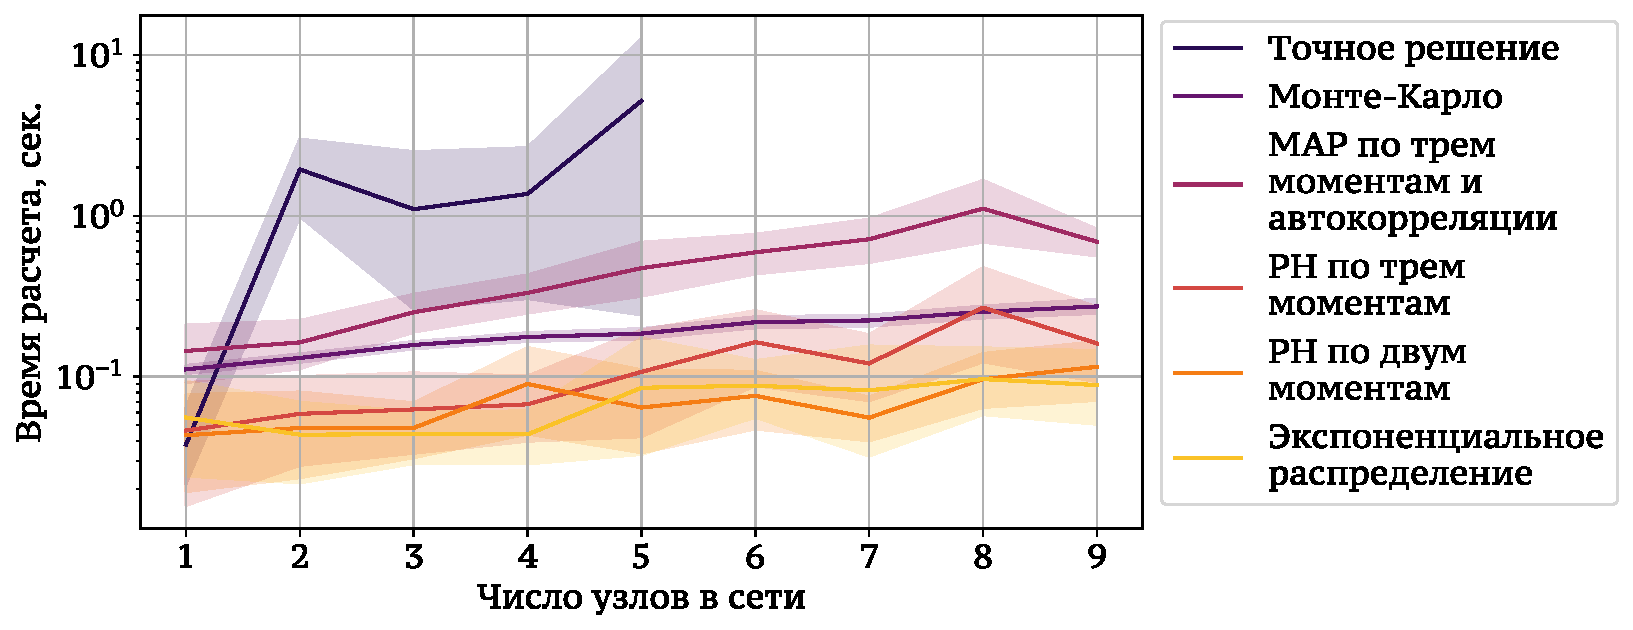
\includegraphics[width=0.90\textwidth]{chapter4/ch4_approximations_elapsed}
    \end{center}
    \footnotesize
    \begin{itemize}
        \item Точный расчет требует очень много времени из-за экспоненциального роста порядков MAP-потоков.
        \item Аппроксимация MAP-потоками по трем моментам и коэффициенту корреляции требует больше времени, чем метод Монте-Карло.
        \item Для небольших сетей аппроксимация PH-распределениями по двум и трем моментам работает значительно быстрее метода Монте-Карло.
    \end{itemize}
\end{frame}

\begin{frame}
    \frametitle{Построение модели беспроводной сети IEEE 802.11}
    \begin{center}
        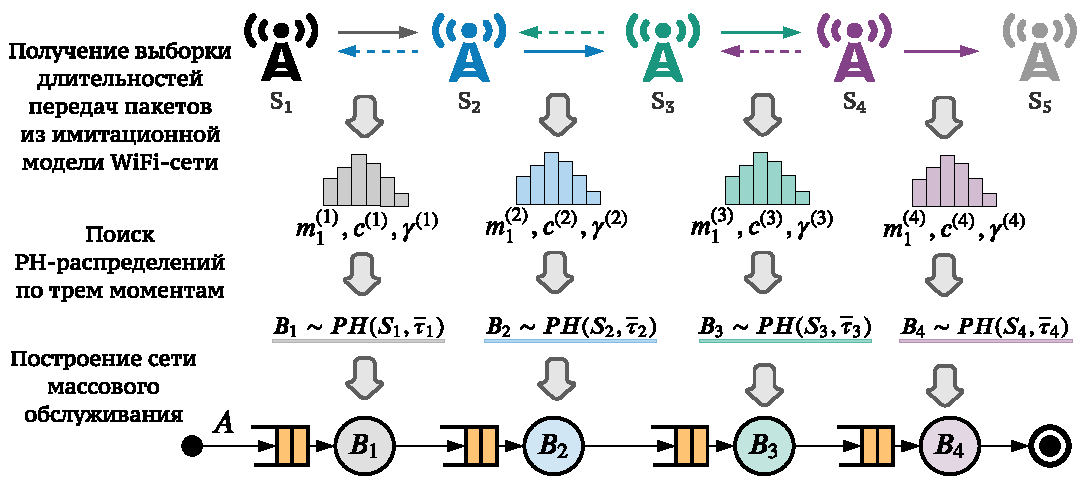
\includegraphics[width=0.8\textwidth]{chapter4/ch4_channel_model_schema.pdf}
    \end{center}
    \footnotesize
    \begin{itemize}
        \item Распределение времени обслуживания должно учитывать периоды ожидания станцией освобождения канала, повторные передачи, ожидание подтверждений, отражать распределение размеров передаваемых пакетов.
        \item Для построения PH-распределений, моделирующих длительность передачи в каналах многошаговой сети, предлагается использовать калибровочную сеть фиксированного размера.
        \item Число станций калибровочной сети выбирается таким образом, чтобы учесть разнообразные условия конкуренции за право доступа к каналу.
        \item В диссертационном исследовании калибровочная сеть включает пять станций.
    \end{itemize}
    % \begin{center}
    %     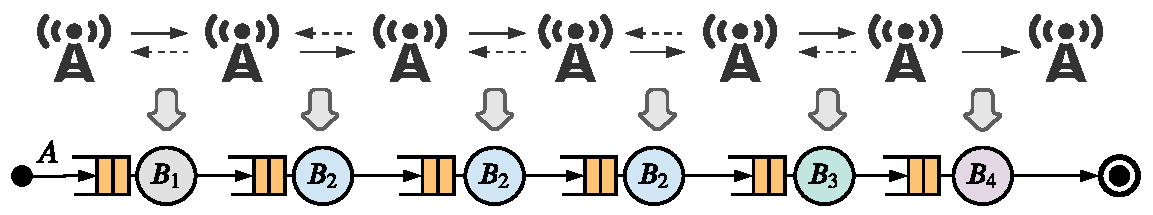
\includegraphics[width=0.8\textwidth]{chapter4/ch4_network_model_schema.pdf}
    % \end{center}
\end{frame}

\begin{frame}
    \frametitle{Методика моделирования беспроводной сети}
    \footnotesize
    Основываясь на числе станций, с которыми конкурируют станции сети, была предложена следующая методика выбора PH-распределений для моделирования каналов сети произвольного размера:
    \begin{center}
        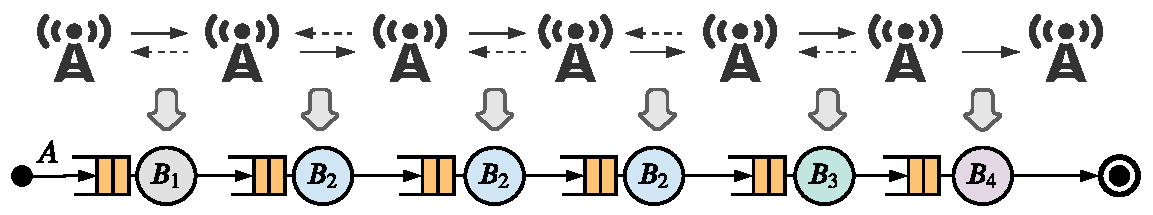
\includegraphics[width=0.6\textwidth]{chapter4/ch4_network_model_schema}
    \end{center}

    \footnotesize
    Для различных интенсивностей входящего трафика были получены оценки межконцевых задержек с помощью имитационной модели в системе NS-3 и сетей массового обслуживания. Распределения времени обслуживания вычислялись по выборке интервалов, полученной из имитационной модели калибровочной сети, реализованной в NS-3.
    \begin{center}
        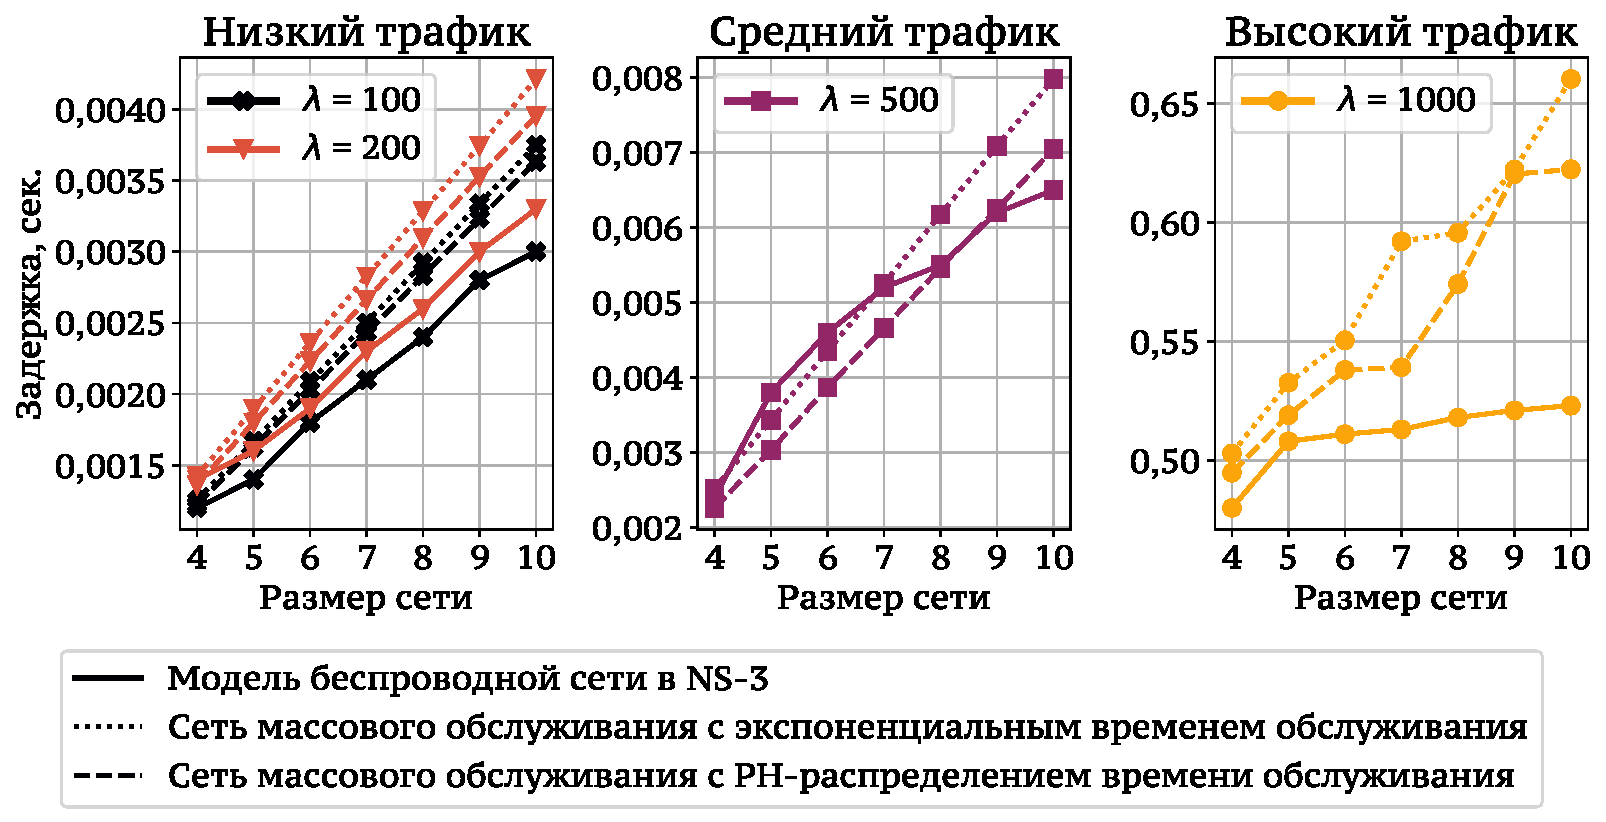
\includegraphics[width=0.7\textwidth]{chapter4/ch4_ns3_tandem_delays}
    \end{center}
\end{frame}


\begin{frame}
    \frametitle{Уточнение методики моделирования беспроводной сети}
    \footnotesize
    Для определения причины большой погрешности при высокой интенсивности были исследованы задержки и вероятности потери пакетов в каналах сети с десятью станциями. Эксперимент показал, что большая часть пакетов теряется на первых четырех станциях, после чего средняя задержка практически не меняется.
    \begin{center}
        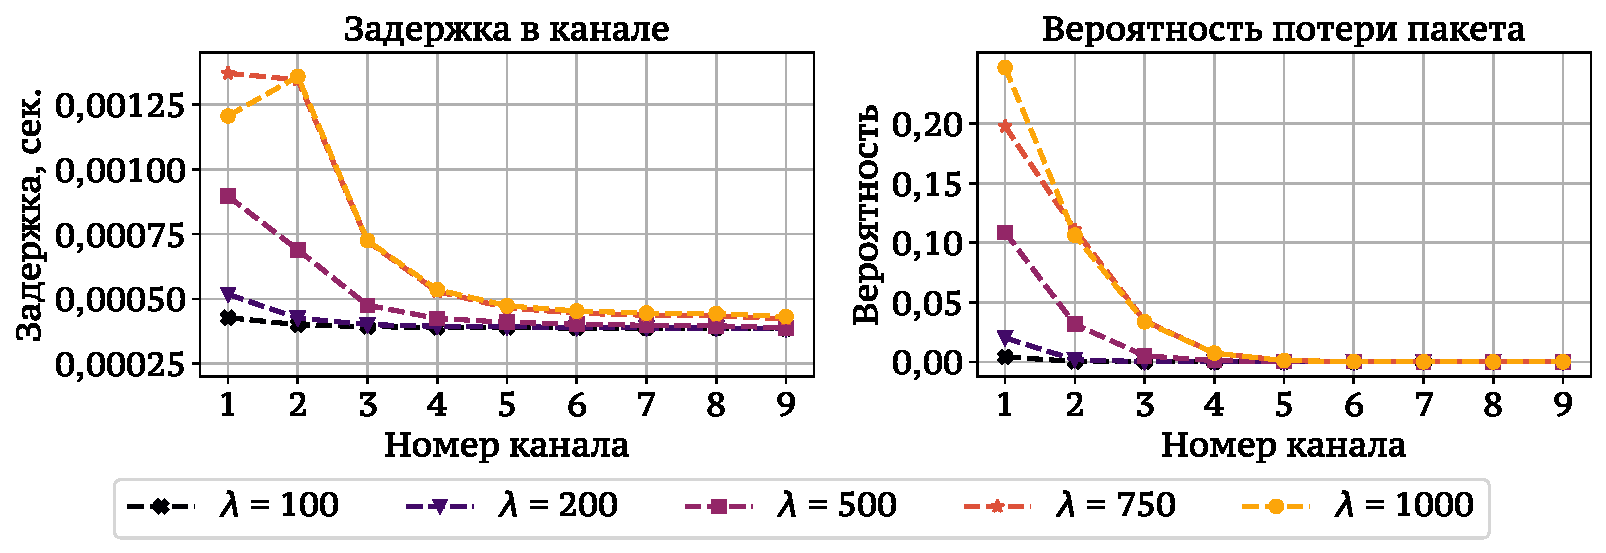
\includegraphics[width=0.8\textwidth]{chapter4/ch4_ns3_net_10_props}
    \end{center}

    \footnotesize
    Чтобы учесть это наблюдение было решено изменить методику выбора PH-распределений, найденных с помощью калибровочной сети, следующим образом:
    \begin{center}
        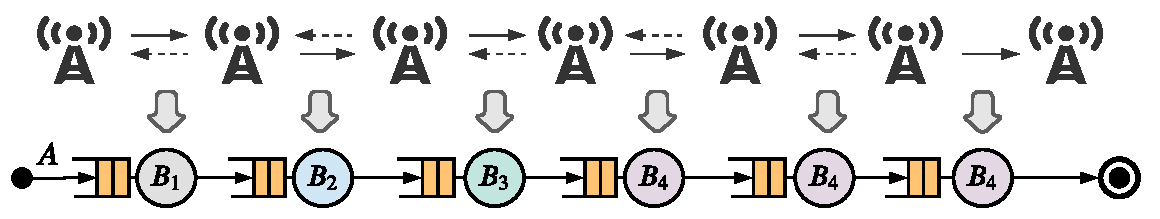
\includegraphics[width=0.6\textwidth]{chapter4/ch4_network_model_schema_refined}
    \end{center}
\end{frame}

\begin{frame}
    \frametitle{Результаты оценки межконцевых задержек}
    \begin{columns}
        \begin{column}{0.65\textwidth}
            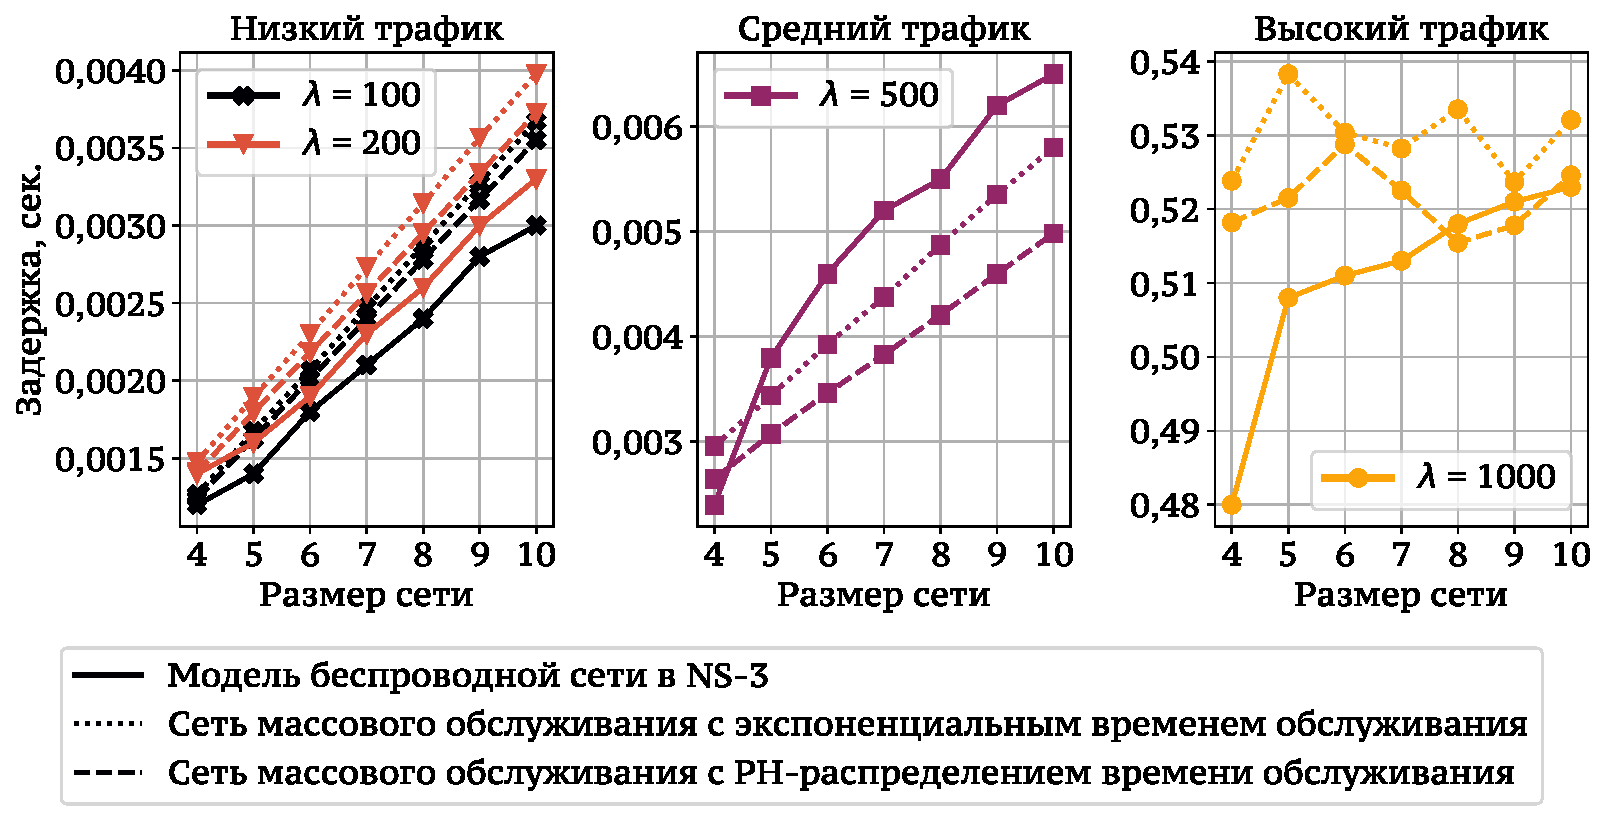
\includegraphics[width=\textwidth]{chapter4/ch4_ns3_tandem_delays_refined.pdf}
            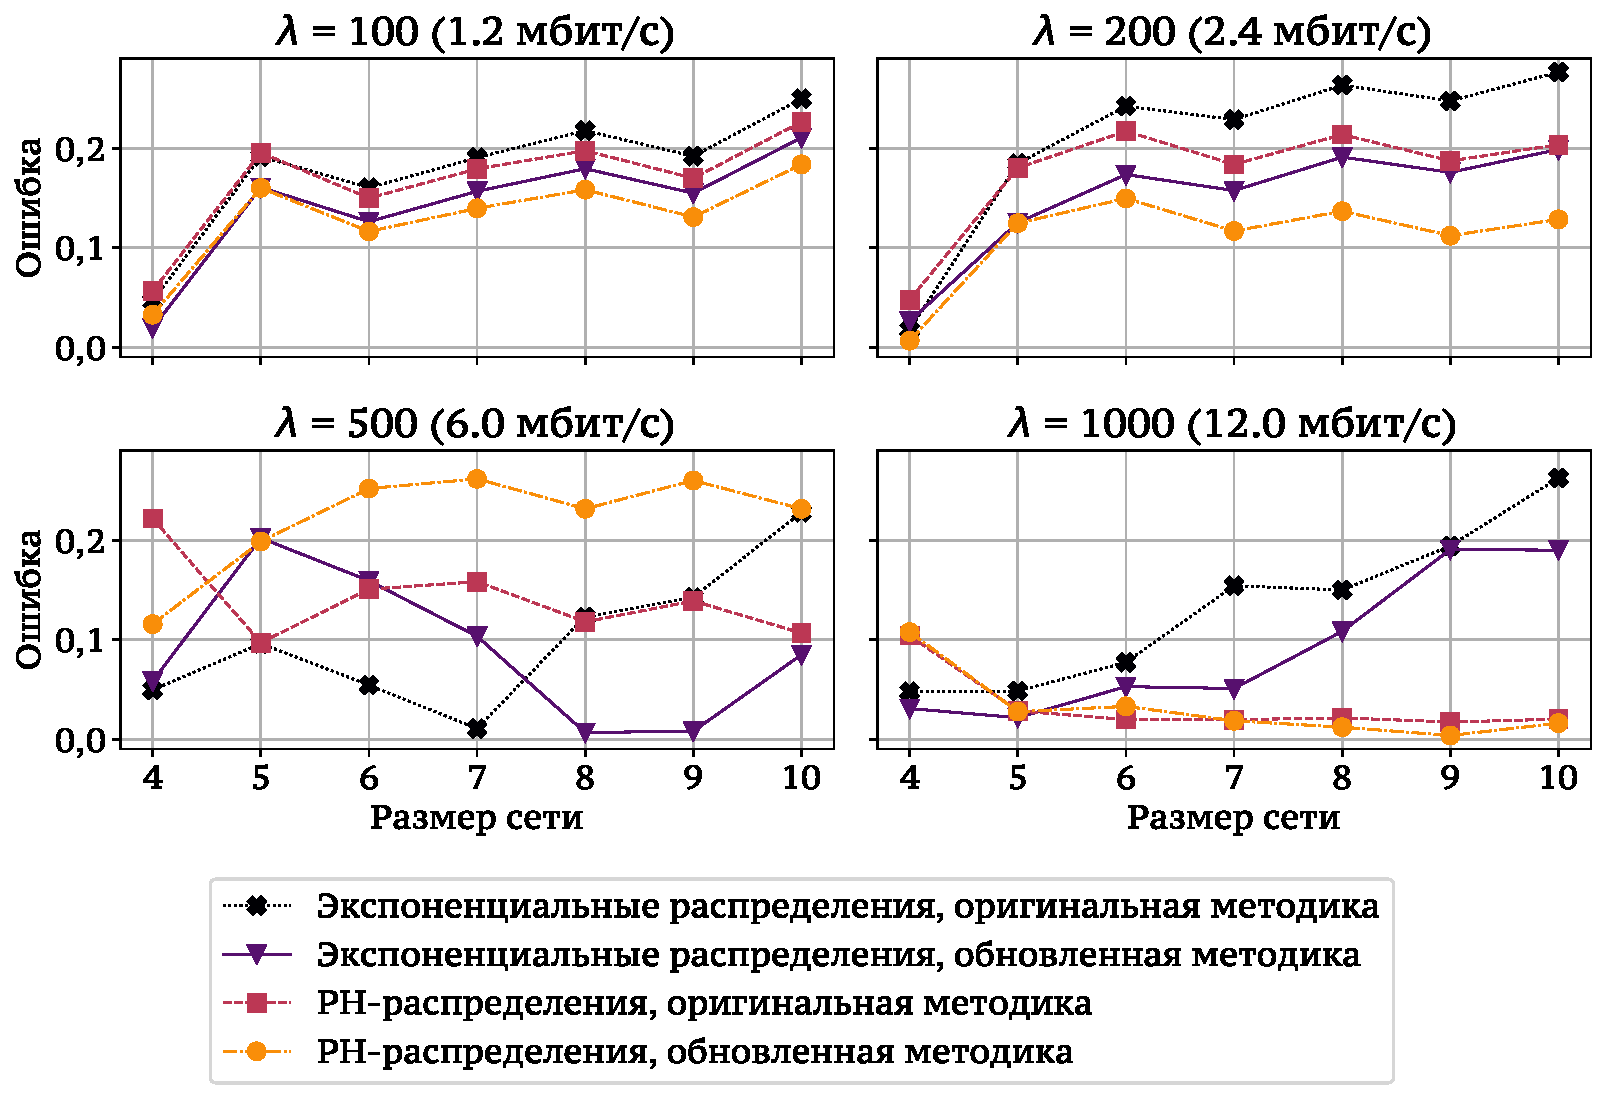
\includegraphics[width=\textwidth]{chapter4/ch4_ns3_tandem_errors.pdf}
        \end{column}
        \begin{column}{0.32\textwidth}
            \footnotesize
            \begin{itemize}
                \item Обновленная методика позволяет вычислять более точные оценки.
                \item Методика позволяет вычислять оценки межконцевых задержек с точностью $ \geqslant 0,8$.
                \item Вычисление с помощью предложенной методики требует значительно меньше времени, чем моделирование в NS-3.
            \end{itemize}
        \end{column}
    \end{columns}
\end{frame}

\begin{frame}
    \frametitle{Выводы}
    \small
    \begin{itemize}
        \item Предложен метод нахождения приближенных значений характеристик открытых сетей массового обслуживания с узлами MAP/PH/1/N с помощью аппроксимации потоков обслуженных пакетов PH-распределениями и MAP-потоками меньшего порядка. Приведены результаты численного исследования метода, показывающие высокую точность при использовании PH-распределений, построенных по трем моментам исходного потока.
        \item Предложена методика построения и выбора распределений для моделирования многошаговых беспроводных сетей IEEE 802.11 произвольного размера с помощью тандемных сетей массового обслуживания.
        \item Представлены результаты численного исследования предложенной методики моделирования многошаговых беспроводных сетей, показывающие высокую точность получаемых оценок межконцевых задержек.
    \end{itemize}
    \footnotesize
    Все модели, документация и численные эксперименты доступны на сайте \url{https://github.com/larioandr/thesis-queues}
\end{frame}


% ============================================================================
% ЧАСТЬ 5. РАЗРАБОТКА И ЭКСПЕРИМЕНТАЛЬНОЕ ВНЕДРЕНИЕ СИСТЕМЫ РАДИОЧАСТОТНОЙ
%          ИДЕНТИФИКАЦИИ
% ============================================================================
\section{Разработка и экспериментальное внедрение системы радиочастотной идентификации}
\begin{frame}[plain, noframenumbering]
    \begin{center}
        \Huge
        Разработка и экспериментальное внедрение системы радиочастотной идентификации
    \end{center}
\end{frame}

\begin{frame}
    \frametitle{Постановка задачи}
    Для исследования практической эффективности системы радиочастотной идентификации была решена следующая задача.
    \begin{alertblock}{Задача}
        Разработать архитектуры и реализовать распределенную системы управления и сбора данных с RFID-считывателей, произвести ее экспериментальное внедрение и осуществить проведение испытаний.
    \end{alertblock}
\end{frame}

\begin{frame}
    \frametitle{Архитектура распределенной системы управления}
    Система включает четыре типа компонентов:
    \begin{columns}
        \begin{column}{0.5\textwidth}
            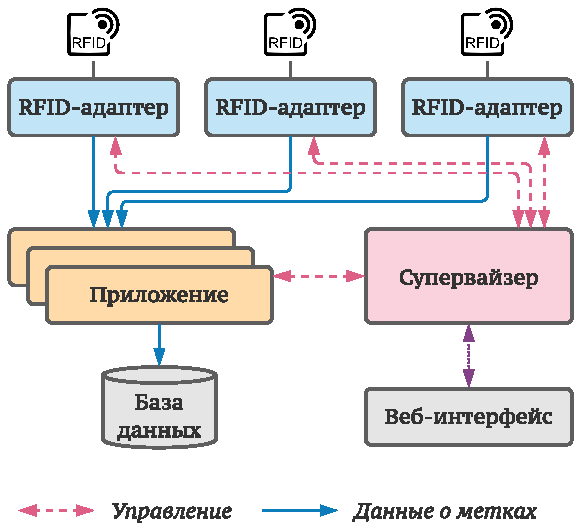
\includegraphics [width=\textwidth]{chapter5/ch5_components}
        \end{column}
        \begin{column}{0.48\textwidth}
            \footnotesize
            \begin{itemize}
                \item Супервайзер (SVR): управляет конфигурацией системы, осуществляет авторизацию запросов.
                \item RFID-адаптеры: взаимодействуют с радиомодулями RFID, предоставляет возможность подписываться на потоки считанных меток или выполнять иные операции над метками.
                \item Приложения: компоненты, осуществляющие преобразования потоков считанных меток.
                \item Пользовательские интерфейсы (командной строки, веб-интерфейс).
            \end{itemize}
        \end{column}
    \end{columns}
\end{frame}

\begin{frame}
    \frametitle{Способы размещения компонентов}
    \begin{center}
        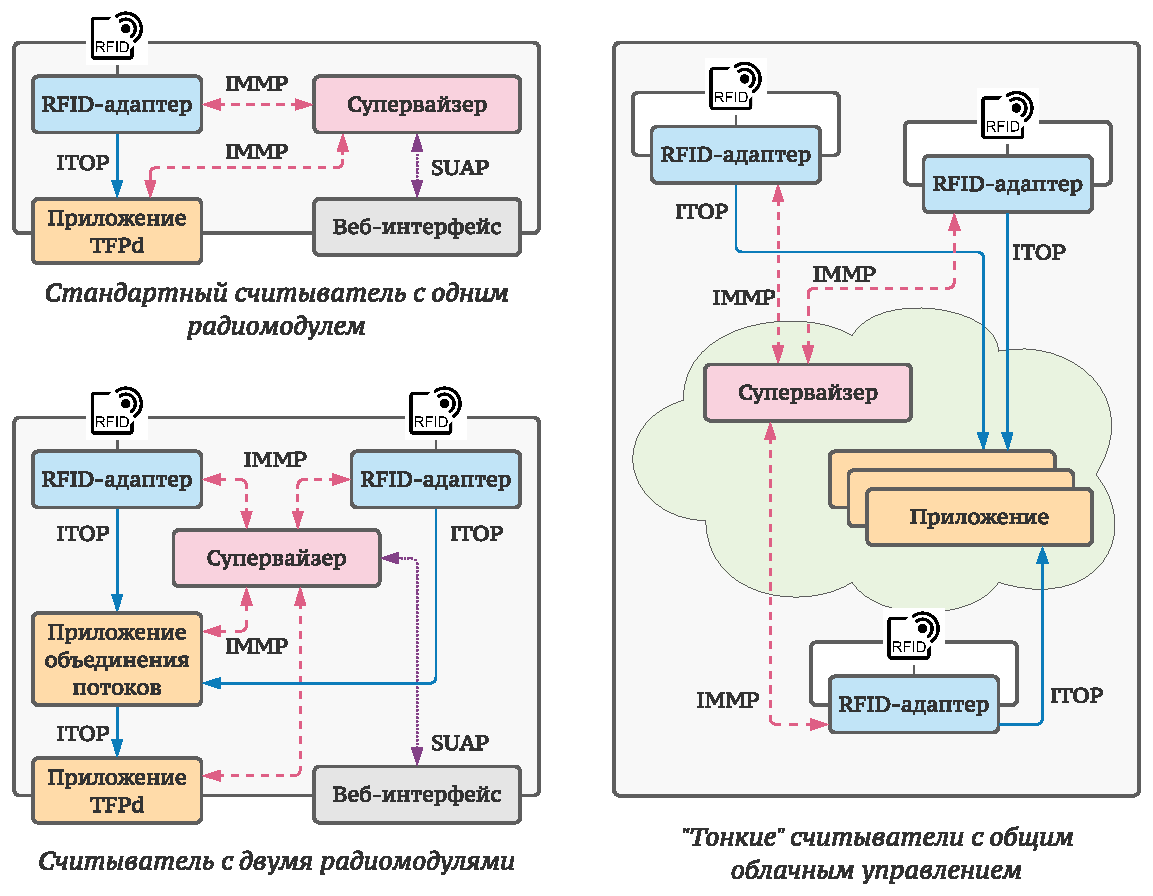
\includegraphics [width=0.7\textwidth]{chapter5/ch5_deployments}
    \end{center}
    \footnotesize
    Все компоненты взаимодействуют друг с другом с помощью протоколов, использующих TCP или UDP. Компоненты могут размещаться на одном или различных компьютерах. Возможно размещение компонентов в облаке.
\end{frame}

\begin{frame}
    \frametitle{Протоколы связи между компонентами}
    Для системы управления были разработаны четыре протокола:
    \begin{columns}
        \begin{column}{0.35\textwidth}
            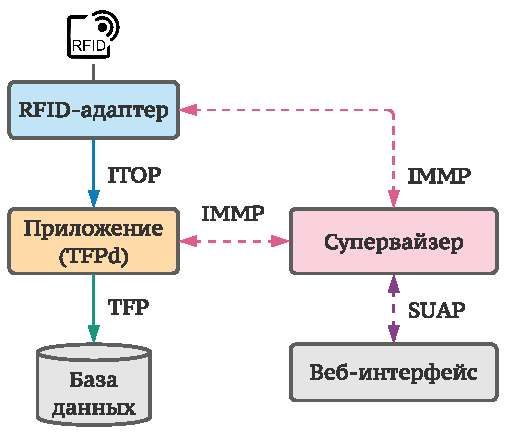
\includegraphics [width=\textwidth]{chapter5/ch5_protocols}
        \end{column}
        \begin{column}{0.64\textwidth}
            \footnotesize
            \begin{itemize}
                \item IMMP (Internal Modules Management Protocol): протокол управления компонетами системы (TCP).
                \item SUAP (Simple User-Access Protocol): протокол управления для подключения пользовательских интерфейсов (UDP).
                \item ITOP (Internal Tag Operation Protocol): протокол, предоставляющий операции чтения и записи меток, а также создания подписки на поток считанных меток (TCP).
                \item TFP (Tag Flow Protocol): простой протокол передачи потока считанных меток, используется для подключения внешних пользователей к системе.
            \end{itemize}
        \end{column}
    \end{columns}
\end{frame}

% \begin{frame}
%     \frametitle{Протокол управления компонентами IMMP}
% \end{frame}

% \begin{frame}
%     \frametitle{Протокол работы с RFID-адаптерами ITOP}
% \end{frame}

% \begin{frame}
%     \frametitle{Протокол подключения абонентов TFP}
% \end{frame}

% \begin{frame}
%     \frametitle{Протокол подключения интерфейсов SUAP}
% \end{frame}

\begin{frame}
    \frametitle{Организация параллельной обработки в RFID-адаптере}
    \begin{center}
        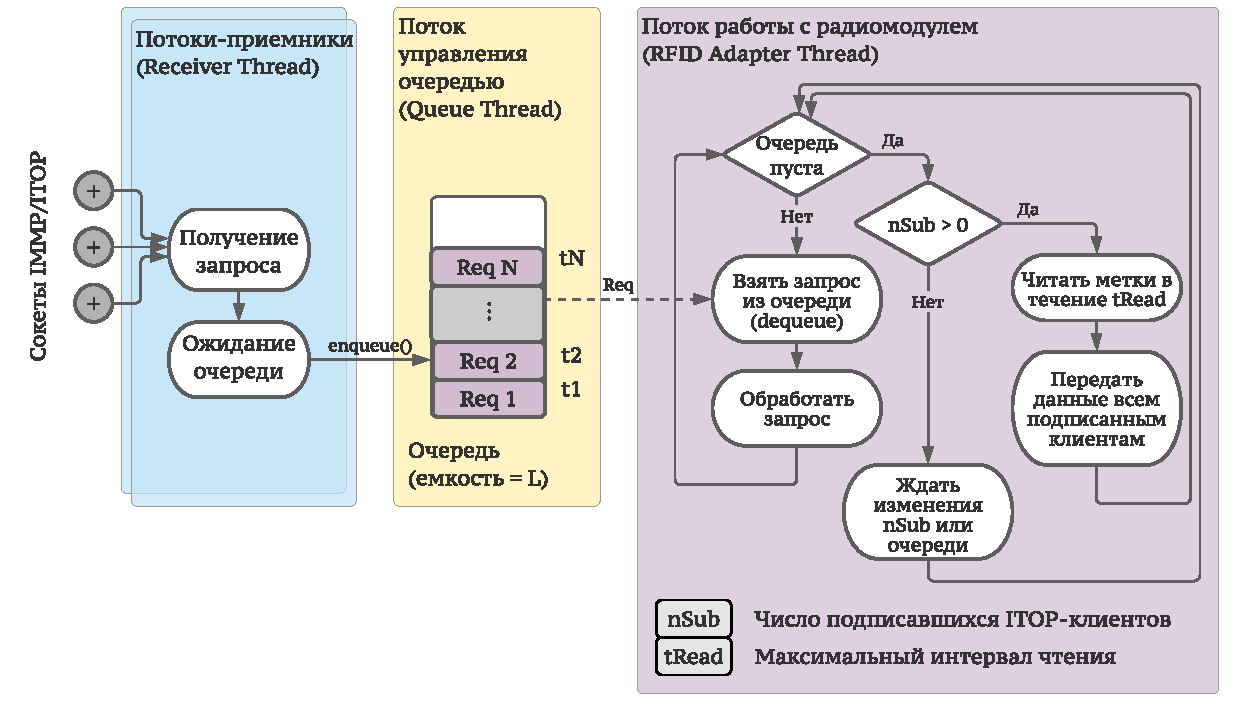
\includegraphics [width=1.0\textwidth] {chapter5/ch5_g2rd_threads}
    \end{center}
\end{frame}

\begin{frame}
    \frametitle{Особенности реализации системы}
    \small
    \begin{itemize}
        \item Все компоненты системы, кроме веб-интерфейса, реализованы на C++.
        \item Обработка запросов в каждом из компонентов осуществляется множеством потоков-рабочих.
        \item Запросы каждого из протоколов поступают в очередь конечной емкости и имеют директивный срок. Если запрос ждет в очереди слишком долго, он удаляется, а клиенту передается сообщение об ошибке.
        \item Подписка на потоки не затрагивает SVR.
        \item Если подписок на поток меток нет, RFID-адаптер отключает считыватель для экономии энергии.
    \end{itemize}
\end{frame}

\begin{frame}
    \frametitle{Структура RFID-считывателя}
    \begin{center}
        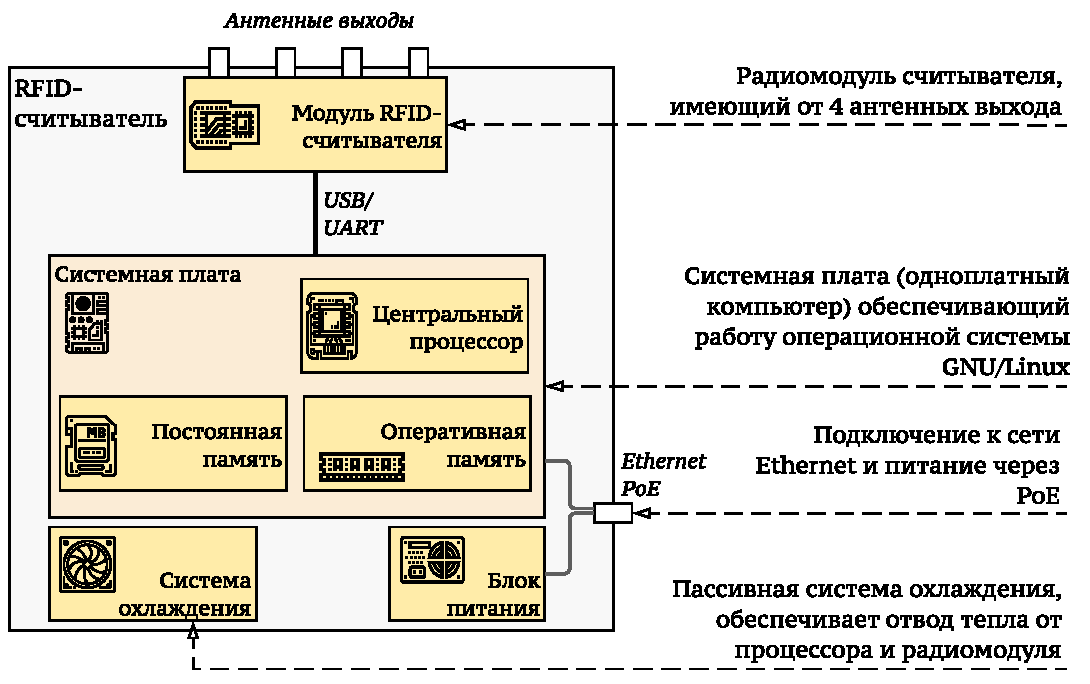
\includegraphics [width=0.7\textwidth] {chapter5/ch5_reader_hardware}
    \end{center}
    \footnotesize
    \begin{itemize}
        \item Считыватель состоит из одноплатного компьютера, радиомодуля RFID и модуля питания.
        \item Одноплатный компьютер построен на четырехядерном процессоре Exynos4412 Prime 1,7~ГГц ARM Cortex-A9, имеет 2~ГБ оперативной памяти LP-DDR2, интерфейс FastEthernet 100~Мб/с и сменную карту памяти 8~ГБ.
        \item Питание осуществляется через интерфейс Ethernet.
        \item Радиомодуль RFID имеет четыре антенных порта, подключается через интерфейс USB, обеспечивает выходную мощность до 31,5~дБм.
    \end{itemize}
\end{frame}

\begin{frame}
    \frametitle{Эксперимент №1: Казань, 2014 год}
    \begin{columns}
        \begin{column}{0.55\textwidth}
            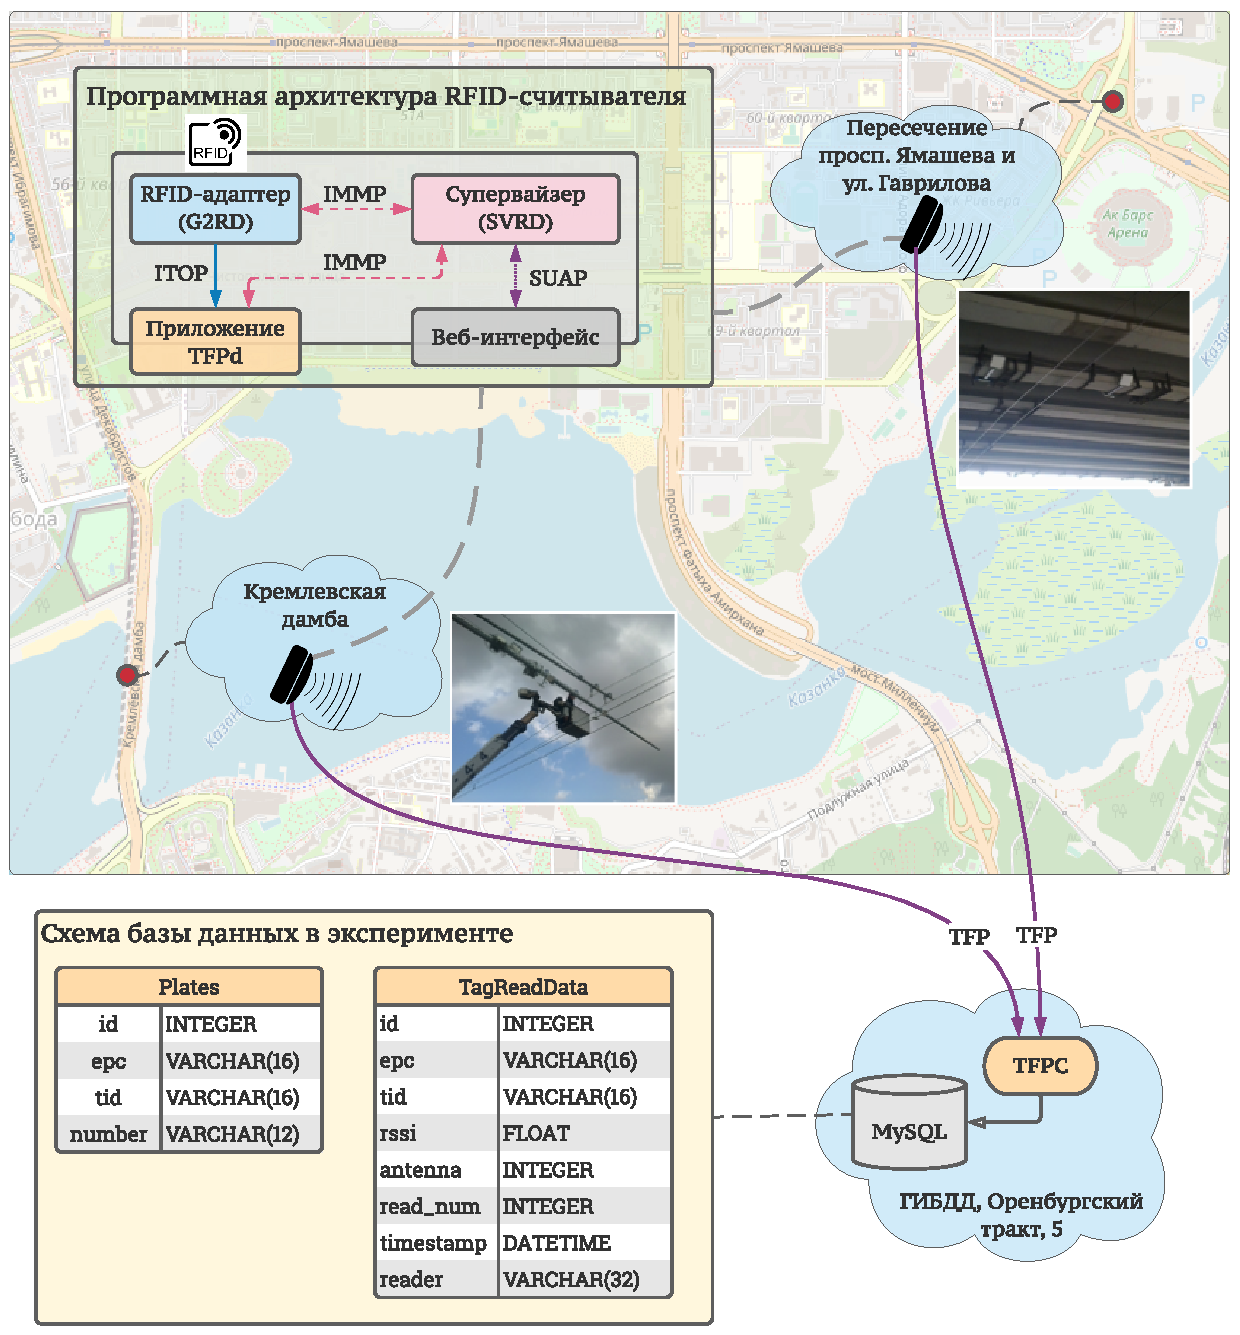
\includegraphics [width=\textwidth] {chapter5/ch5_kazan2014_schema}
        \end{column}
        \begin{column}{0.44\textwidth}
            \footnotesize
            \begin{itemize}
                \item Впервые в РФ был проведен масштабный эксперимент внедрения RFID в номерные знаки.
                \item Метками производства NXP были оснащены 740 автобусов. Знаки c метками были произведены ООО <<Знак>> по технологии фирмы Tonnjes Group Gmbh.
                \item RFID-считывателями были оборудованы четыре точки, две из них "--- оборудованием, разработанным в диссертационной работе.
                \item Данные о считанных метках поступали в ЦОД.
                \item Результаты валидировались независимым наблюдением.
                \item Вероятность идентификации: \textbf{92 -- 95~\%}.
            \end{itemize}
        \end{column}
    \end{columns}
\end{frame}

\begin{frame}
    \frametitle{Эксперимент №2: Казань, 2020 год}
    \footnotesize
    В 2020 году в рамках НИР <<Знак-Метка>>, разработанного по указанию вице-премьера РФ Борисова Ю.И., были проведены испытания на полигоне ИТС ООО <<Казань-Телематика>> в г. Казань. В испытаниях использовался разработанный RFID-считыватель и метки в номерных знаках производства ПАО <<Микрон>>.
    \begin{columns}
        \begin{column}{0.68\textwidth}
            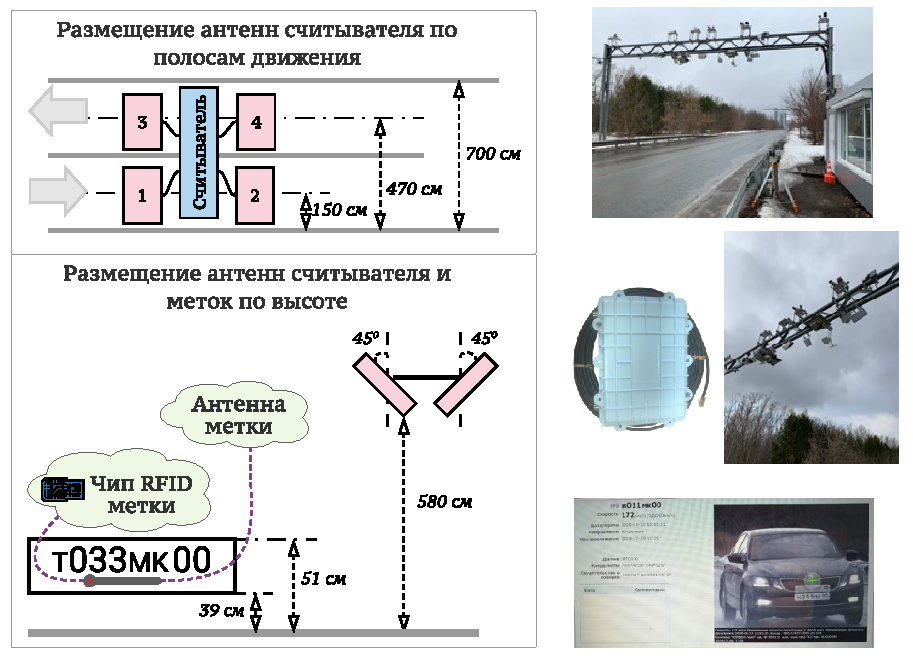
\includegraphics [width=\textwidth] {chapter5/ch5_kazan2020_schema}
        \end{column}
    \end{columns}
    \footnotesize
    Скорость движения автомобилей в эксперименте составляла от 60 до 172 км/ч, а также исследовалась идентификация при маневрах обгона и следования. Все метки были успешно идентифицированы.
\end{frame}

\begin{frame}
    \frametitle{Эксперимент №3: ЦКАД, 2021 год}
    \footnotesize
    В 2021 году совместно с ПАО <<Микрон>> были проведены испытания RFID на платном участке центральной кольцевой автодороги (ЦКАД). Целью эксперимента являлась проверка возможности использования UHF RFID для оплаты проезда по платной дороге и проверка точности позиционирования автомобиля.
    \vfill
    В эксперименте использовалось то же оборудование и программное обеспечение, которое использовалось в эксперименте 2020 года. С учетом особенностей меток, считыватель был настроен на чтение 96 бит TID.
    \vfill
    Основные выводы:
    \begin{itemize}
        \item \footnotesize При установке считывателей на большой высоте необходимо использовать высокую выходную мощность (согласуется с результатами модели).
        \item Сторонние метки установлены на большом количестве автомобилей (предположительно, на лобовых стеклах, товарах в кузове), поэтому важно обеспечить эффективную фильтрацию и использовать $Q > 2$ для предотвращения коллизий.
    \end{itemize}
\end{frame}

\begin{frame}
    \frametitle{Выводы}
    \footnotesize
    \begin{itemize}
        \item Разработана распределенная система управления RFID-считывателями. Для управления и передачи данных в системе используются различные протоколы, позволяющие избежать перегрузки системы при увеличении числа RFID-считывателей. Система управления обладает высокой гибкостью, позволяет реализовывать на ее основе считыватели различной конфигурации.
        \item Проведены три экспериментальных испытания системы: в 2014 и в 2020 годах в Казани, и в 2021 году в Московской области на ЦКАД. Успешные результаты испытаний показывают, что разработанную систему радиочастотной идентификации можно использовать для регистрации автомобилей, движущихся с большими скоростями и совершающих различные маневры на дороге.
        \item Полученные результаты экспериментов согласуются с теоретическими результатами, представленными в диссертационной работе. Отмечено, что для эффективного использования системы желательно иметь выделенные каналы связи, для построения которых можно использовать многошаговые беспроводные сети.
    \end{itemize}
\end{frame}

% % ============================================================================
% % ЧАСТЬ 6. ЗАКЛЮЧЕНИЕ
% % ============================================================================
% \section{Заключение}



% ============================================================================
% ЧАСТЬ -. ПРИМЕРЫ
% ============================================================================
% \section{-- Примеры --}
% \begin{frame}[plain, noframenumbering]
%     \begin{center}
%         \Huge
%         ПРИМЕРЫ ИЗ ПАКЕТА PHD-THESIS-LATEX
%     \end{center}
% \end{frame}
% \begin{frame}[plain, noframenumbering]
%     \begin{center}
%         \Huge
%         Графика
%     \end{center}
% \end{frame}


% \begin{frame}[plain, noframenumbering]
%     \frametitle{Одиночное изображение}
%     \centering
%     \includegraphics[width=0.8\linewidth]{latex} % окружение figure не требуется
% \end{frame}

% \begin{frame}[plain, noframenumbering]
%     \frametitle{Векторная графика}
%     \begin{figure}
% 	    \centering
% 	    \ifdefmacro{\tikzsetnextfilename}{\tikzsetnextfilename{tikz_presentation}}{}% присваиваемое предкомпилированному pdf имя файла (не обязательно)
% 	    \input{Presentation/images/tikz_plot.tikz}
%     \end{figure}
% \end{frame}


% \begin{frame}[plain, noframenumbering]
%     \frametitle{Изображения по-вертикали}
%     \centering
%     \vfill
%     \includegraphics[width=0.8\linewidth,height=0.1\textheight]{latex} \\
%     \TeX
%     \vfill
%     \includegraphics[width=0.8\linewidth,height=0.2\textheight]{latex} \\
%     \LaTeX
%     \vfill
%     \includegraphics[scale=0.2]{latex} \\
%     \vfill
% \end{frame}


% \begin{frame}[plain, noframenumbering]
%     \frametitle{Изображения по-горизонтали}
%     \begin{minipage}[t]{0.47\linewidth}
%         \textbf{Составная \\ подпись 1}
%         \center{\includegraphics[width=1\linewidth]{knuth1}}
%     \end{minipage}
%     \hfill
%     \begin{minipage}[t]{0.47\linewidth}
%         \textbf{Составная \\ подпись 2}
%         \center{\includegraphics[width=1\linewidth]{knuth2}}
%     \end{minipage}
% \end{frame}

% \begin{frame}[plain, noframenumbering]
%     \frametitle{Разделяющие линии}
%     \begin{minipage}[c]{0.47\linewidth}
%         \center{\includegraphics[width=1\linewidth]{latex}}
%         \bigskip
%         \hrule{}
%         \bigskip
%         \textbf{Составная \\ подпись 1}
%     \end{minipage}
%     \hfill
%     \vrule{}
%     \hfill
%     \begin{minipage}[c]{0.47\linewidth}
%         \flushright
%         \textbf{Составная \\ подпись 2}
%         \center{\includegraphics[width=1\linewidth]{knuth2}}
%     \end{minipage}
% \end{frame}

% \begin{frame}[plain, noframenumbering]
%     \begin{center}
%         \Huge
%         Остальное
%     \end{center}
% \end{frame}


% \begin{frame}[plain, noframenumbering]
%     \frametitle{Формулы}
%     \[
%     \left\{
%     \begin{array}{rl}
%         \dot x = & \sigma (y-x)  \\
%         \dot y = & x (r - z) - y \\
%         \dot z = & xy - bz
%     \end{array}
%     \right.
%     \]
% \end{frame}

% \begin{frame}[plain, noframenumbering]
%     \frametitle{amsmath}
%     \centering
%     \begin{minipage}[t]{0.5\linewidth}
%         \begin{multline*}
%             y = 1 x^1 + 2 x^2 + 3 x^3 + \\ + 4 x^4 + 5 x^5 + \dots
%         \end{multline*}
%     \end{minipage}
% \end{frame}

% \begin{frame}[allowframebreaks, noframenumbering]
%     \frametitle{Уравнения Максвелла}
%     \centering{
%         \small
%         \def\arraystretch{1.8}%
%         \begin{tabular}{ll}
%             \toprule
%             Интегральная форма                                                                                                                                          & Дифференциальная форма                                                        \\ \midrule
%             \(Q_e(t) = \displaystyle\oiint_S \vec D(t) \cdot d\vec{s} = \displaystyle\iiint_V \rho_v(t) dv\)                                                              & \(\nabla \cdot \vec D(t) = \rho_v(t)\)                                          \\
%             \(\displaystyle\oiint_S \vec B(t) \cdot d\vec{s} = 0\)                                                                                                        & \(\nabla \cdot \vec B(t) = 0\)                                                  \\
%             \(V_{emf}(t) = \displaystyle\oint_L \vec E(t) \cdot d\vec{l}\) = \(- \displaystyle\iint_S \left[\frac{\partial\vec{B}(t)}{\partial t}\right] \cdot d\vec{s}\)   & \(\nabla \times \vec E(t) = - \frac{\partial\vec{B}(t)}{\partial t}\)           \\
%             \(I(t) = \displaystyle\oint_L \vec H(t) \cdot d\vec{l} = \displaystyle\iint_S \left[\vec J(t) + \frac{\partial\vec{D}(t)}{\partial t}\right] \cdot d\vec{s}\) & \(\nabla \times \vec H(t) = \vec J(t) + \frac{\partial\vec{D}(t)}{\partial t}\) \\ \midrule
%             \(\displaystyle\oiint_S \vec J \cdot d\vec{s} = -\frac{\partial Q_e}{\partial t}\)                                                                            & \(\nabla \cdot \vec J = - \frac{\partial \rho_v}{\partial t}\)                  \\
%             \bottomrule
%             \multicolumn{2}{c}{\(\vec D(t) = \left[\varepsilon(t)\right] * \vec E(t)\)}                                                                                                                                                                   \\
%             \multicolumn{2}{c}{\(\vec B(t) = \left[\mu(t)\right] * \vec H(t)\)}                                                                                                                                                                           \\
%         \end{tabular}
%     }
%     \framebreak

%     \hspace{0.05\linewidth}
%     \centering{
%         \small
%         \def\arraystretch{1.8}%
%         \begin{tabular}{ll}
%             \toprule
%             Интегральная форма                                                                                                            & Дифференциальная форма                             \\ \midrule
%             \(Q_e = \displaystyle\oiint_S \vec D \cdot d\vec{s} = \displaystyle\iiint_V \rho_v dv\)                                         & \(\nabla \cdot \vec D = \rho_v\)                     \\
%             \(\displaystyle\oiint_S \vec B \cdot d\vec{s} = 0\)                                                                             & \(\nabla \cdot \vec B = 0\)                          \\
%             \(V_{emf} = \displaystyle\oint_L \vec E \cdot d\vec{l}\) = \(- \displaystyle\iint_S \left[j \omega \vec B\right] \cdot d\vec{s}\) & \(\nabla \times \vec E = - j \omega \vec B\)         \\
%             \(I = \displaystyle\oint_L \vec H \cdot d\vec{l} = \displaystyle\iint_S \left[\vec J + j \omega \vec D\right] \cdot d\vec{s}\)  & \(\nabla \times \vec H = \vec J + j \omega \vec{D}\) \\ \midrule
%             \(\displaystyle\oiint_S \vec J \cdot d\vec{s} = - j \omega Q_e\)                                                                & \(\nabla \cdot \vec J = - j \omega \rho_v\)          \\
%             \bottomrule
%             \multicolumn{2}{c}{\(\vec D(t) = \left[\varepsilon\right] \vec E(t)\)}                                                                                                               \\
%             \multicolumn{2}{c}{\(\vec B(t) = \left[\mu\right] \vec H(t)\)}                                                                                                                       \\
%         \end{tabular}
%     }
% \end{frame}

% \begin{frame}[plain, noframenumbering]
%     \frametitle{Таблица}
%     \centering
%     \begin{tabular}{|l|l|}
%         \hline
%         \textbf{Заголовок 1} & \textbf{Заголовок 2} \\
%         \hline
%         Сумма                & \(b+a\)                \\
%         \hline
%         Разность             & \(a-b\)                \\
%         \hline
%         Произведение         & \(a*b\)                \\
%         \hline
%     \end{tabular}
% \end{frame}

% \begin{frame}[plain, noframenumbering]
%     \frametitle{Другая таблица}
%     \centering
%     \begin{tabular}{lc}
%         \toprule
%         \multicolumn{1}{c}{\textbf{Заголовок 1}} & \textbf{Заголовок 2} \\ \midrule
%         Сумма                                    & \(b+a\)                \\
%         Разность                                 & \(a-b\)                \\
%         Произведение                             & \(a*b\)                \\
%         \bottomrule
%     \end{tabular}
% \end{frame}


% \begin{frame}[plain, noframenumbering]
%     \frametitle{Большой многоуровневый список}
%     \begin{itemize}
%         \item \textbf{Пункт 1}
%               \begin{itemize}
%                   \itemi Подпункт 1-1
%                   \itemi Подпункт 1-2
%               \end{itemize}
%         \item \textbf{Пункт 2}
%               \begin{itemize}
%                   \itemi Подпункт 2-1
%               \end{itemize}
%         \item \textbf{Пункт 3}
%               \begin{itemize}
%                   \itemi Подпункт 3-1
%                   \itemi Подпункт 3-2
%               \end{itemize}
%         \item \textbf{Пункт 4}
%               \begin{itemize}
%                   \itemi Подпункт 4-1
%               \end{itemize}
%         \item \textbf{Пункт 5}
%               \begin{itemize}
%                   \itemi Подпункт 5-1
%                   \itemi Подпункт 5-2
%                   \itemi Подпункт 5-3
%               \end{itemize}
%     \end{itemize}
% \end{frame}

% \begin{frame}[plain, noframenumbering]
%     \frametitle{Четыре изображения}
%     \centering
%     \includegraphics[width=0.35\linewidth,angle=35]{latex}
%     \includegraphics[width=0.35\linewidth,angle=135]{latex}\\
%     \includegraphics[width=0.35\linewidth,angle=15]{latex}
%     \includegraphics[width=0.35\linewidth,angle=-15]{latex}
% \end{frame}

% \begin{frame}[allowframebreaks]
%     \frametitle{Списки}
%     \begin{itemize}
%         \item Проблема 1
%         \item Проблема 2
%         \item Проблема 3
%     \end{itemize}
%     \framebreak
%     \begin{enumerate}
%         \item \textbf{Задача 1}
%               \begin{itemize}
%                   \item Подзадача 1-1
%                   \item Подзадача 1-2
%               \end{itemize}
%         \item \textbf{Задача 2}
%               \begin{itemize}
%                   \item Подзадача 2-1
%                   \item Подзадача 2-2
%                   \item Подзадача 2-3
%               \end{itemize}
%         \item \textbf{Задача 3}
%               \begin{itemize}
%                   \item Подзадача 3-1
%                   \item Подзадача 3-2
%                   \item Подзадача 3-3
%               \end{itemize}
%     \end{enumerate}
%     \framebreak
%     Поясняющий текст
%     \begin{itemize}
%         \item Один
%         \item Два
%         \item Три
%     \end{itemize}
% \end{frame}
% \note[itemize]{
%     \item Тезис 1
%     \item Тезис 2
%     \item Тезис 3
% }
